\chapter{Capa de presentación}
\label{ch:presentacion}

El presente capítulo detalla el diseño y la implementación de la capa de presentación, cuya responsabilidad es proporcionar una interfaz de usuario intuitiva, interactiva, accesible y estéticamente consistente para el Perfil del estudiante.

Este es el capítulo más extenso y, probablemente, el más llamativo. Además de diversos aspectos técnicos correspondientes a la implementación del \gls{frontend}, exhibe y describe minuciosamente la interfaz del Perfil del estudiante, apoyándose en varias capturas de pantalla. Sin embargo, el lector debe tener presente que el desglose que aquí se realiza de la interfaz no suple la experiencia de navegación real en el Perfil del estudiante, directamente en la aplicación web \gls{NES}. Por tanto, se recomienda al lector que, en caso de tener acceso a la aplicación, explore el Perfil del estudiante directamente en ella.

El capítulo se ocupa primeramente de las cuestiones técnicas de la implementación de la capa de presentación, incluyendo el lenguaje y framework utilizados y la estructura de directorios del frontend. Tras eso, se describe, tan bien como es posible en un documento estático, la interfaz interactiva del Perfil del estudiante.

\section{Implementación del frontend}

\subsection{Lenguaje y framework}

El frontend está implementado en el framework \gls{React}, utilizando \gls{TypeScript} como lenguaje principal. El uso de React responde al hecho de que el resto de \gls{NES} está desarrollado bajo ese framework, por lo que se optó por mantener la consistencia con los demás módulos de la aplicación. Se descartó la implementación de microfrontends o alternativas similares puesto que se consideró que introducía complejidad adicional sin aportar beneficios significativos.

Por otro lado, se eligió \gls{TypeScript} por encima de \gls{JavaScript}, debido a que el tipado estático facilita la detección temprana de errores y mejora la mantenibilidad del código. Además, \gls{TypeScript} es un superset de \gls{JavaScript}, lo que garantiza su compatibilidad con el resto de módulos de la aplicación que se encuentran escritos en \gls{JavaScript}.

\subsection{Estructura de directorios del proyecto}

El frontend sigue una arquitectura modular, con el código al interior de la carpeta \lstinline|src| y cada página encapsulada en un directorio dentro de \lstinline|src/pages|. Esto favorece la organización del código y mejora su mantenibilidad. Dado que no compete a este trabajo detallar la estructura de directorios de NES en su totalidad, se describe solo superficialmente la estructura general del frontend, en la tabla \ref{tab:estructura_directorios_frontend}, a modo de contexto.

\begin{longtblr}[
		caption = {Estructura de directorios del proyecto},
		label = {tab:estructura_directorios_frontend},
	]{
		colspec = {X[1,l] X[3,l]}
	}
	\hline
	\textbf{Directorio/Archivo} & \textbf{Descripción}                                                                                                                                         \\
	\hline
	\lstinline|App.tsx|         & Componente principal de la aplicación, que sirve como punto de entrada y organiza las rutas.                                                                 \\
	\lstinline|Router.tsx|      & Configura las rutas de la aplicación, incluyendo la navegación al perfil del estudiante y a las otras páginas.                                               \\
	\lstinline|MainLayout.tsx|  & Componente que define el diseño general de la aplicación, incluyendo el encabezado, pie de página y disposición general.                                     \\
	\lstinline|pages/|          & Directorio que contiene el código asociado a cada página de la aplicación, como el perfil del estudiante.                                                    \\
	\lstinline|hooks/|          & Directorio que almacena hooks reutilizables en toda la aplicación, como manejo del estado global.                                                            \\
	\lstinline|components/|     & Contiene componentes reutilizables que se utilizan en varias páginas.                                                                                        \\
	\lstinline|constants/|      & Define constantes globales del proyecto, como configuraciones y estilos estándar.                                                                            \\
	\lstinline|services/|       & Implementa funciones para interactuar con otros servicios externos (distintos al \gls{API REST} del Perfil del estudiante) que alimentan el frontend.        \\
	\lstinline|assets/|         & Contiene recursos estáticos como imágenes utilizados en la aplicación.                                                                                       \\
	\lstinline|config/|         & Directorio con configuraciones específicas librerías como \gls{axios} y \gls{firebase}.                                                                      \\
	\lstinline|interfaces/|     & Define interfaces de \gls{TypeScript} que se utilizan para tipar datos y garantizar consistencia en el código.                                               \\
	\lstinline|recoilAtoms/|    & Contiene los \textit{atoms} de \gls{Recoil} para el manejo del estado global de la aplicación, que se utilizan para compartir información entre componentes. \\
	\lstinline|utils/|          & Agrupa funciones auxiliares reutilizables en diferentes partes del proyecto.                                                                                 \\
	\lstinline|index.css|       & Archivo principal de estilos CSS utilizado para definir configuraciones de diseño globales.                                                                  \\
	\hline
\end{longtblr}

El código correspondiente al Perfil del estudiante se encuentra en un solo directorio al interior de \lstinline|src/pages|, que es \lstinline|StudentProfilePage|. Naturalmente, en la implementación del Perfil del estudiante se importan y se reutilizan varias utilidades, interfaces, componentes y hooks de las carpetas \lstinline|src/utils|, \lstinline|src/iterfaces|, \lstinline|src/components| y \lstinline|src/hooks|, respectivamente, lo que asegura la consistencia y reduce la duplicación de código.

\subsubsection{Estructura del módulo del Perfil del estudiante}

\sloppy
El módulo del Perfil del estudiante está encapsulado en el directorio \lstinline|src/pages/StudentProfilePage|. Allí, el código a su vez está organizado en un subdirectorios por cada pestaña visual del Perfil del estudiante. Esta organización modulada facilita dos cosas:
\fussy

\begin{itemize}
	\item Realizar cambios de manera localizada, ya que cada pestaña es prácticamente un submódulo independiente.
	\item Asegurar que los permisos de usuario sean administrados correctamente, pues cada pestaña tiene diferentes niveles de acceso. Esto es especialmente importante para la pestaña Financiación, que contiene el detalle de la información financiera del estudiante y, por las políticas de gobierno de datos de la Universidad, solo debe ser accesible para directivos.
\end{itemize}

La estructura de directorios al interior del módulo del Perfil del estudiante se detalla en la tabla \ref{tab:estructura_modulo_perfil}.

\begin{longtblr}[
		caption = {Estructura de directorios del módulo del Perfil del estudiante},
		label = {tab:estructura_modulo_perfil},
	]{
		colspec = {X[2,l] X[3,l]}
	}
	\hline
	\textbf{Directorio/Archivo}       & \textbf{Descripción}                                                                                                 \\
	\hline
	\lstinline|performanceTab/|       & Contiene la pestaña de rendimiento académico.                                                                        \\
	\lstinline|fundingTab/|           & Contiene la pestaña de financiación.                                                                                 \\
	\lstinline|subjectsTab/|          & Contiene la pestaña con todas las materias inscritas por el estudiante.                                              \\
	\lstinline|scheduleTab/|          & Proporciona una vista del horario del estudiante.                                                                    \\
	\lstinline|personalDataCard/|     & Componente que muestra información personal del estudiante y se reutiliza en todas las pestañas.                     \\
	\lstinline|chips/|                & Contiene componentes específicos reutilizados únicamente dentro del perfil del estudiante, como botones y etiquetas. \\
	\lstinline|useStudentProfile.tsx| & Hook que centraliza la obtención de los datos del perfil desde el \gls{API REST}.                                    \\
	\hline
\end{longtblr}

Con respecto a la tabla anterior, cabe señalar que los componentes implementados en \lstinline|chips/| no se implementaron en la carpeta \lstinline|components/| del proyecto debido a que son específicos del Perfil del estudiante y no se reutilizan en otras partes de la aplicación. Dicho eso, en caso de que se requiera reutilizar estos componentes en otras partes de la aplicación, basta con moverlos a la carpeta \lstinline|components/| y ajustar las importaciones correspondientes.

Bajo un raciocinio similar, el hook \lstinline|useStudentProfile.tsx| se implementó dentro del directorio del módulo del Perfil del estudiante, en lugar de en \lstinline|hooks/|, porque se utiliza solamente en el Perfil del estudiante y no en otras partes de la aplicación. Es, además, el único código del frontend que se comunica con el \gls{API REST} del Perfil del estudiante, por lo que su ubicación en el módulo del Perfil del estudiante facilita la comprensión y el mantenimiento del código.

El \lstinline|hook| \lstinline|useStudentProfile.tsx| solicita toda la información relevante del \gls{API REST} del Perfil del estudiante en una única petición. Esto se hace así porque resulta más eficiente. Inicialmente, el diseño del \gls{API} contaba con un endpoint separado para cada recurso, lo que implicaba realizar múltiples peticiones independientes para cada pestaña. Sin embargo, se determinó que esta estructura incrementaba la latencia. Por esta razón, el \gls{API} fue rediseñado para agrupar todos los recursos en una única representación unificada, accesible mediante un solo endpoint.

\subsection{Ruta al perfil del estudiante}
\label{sec:ruta_perfil_estudiante}

Como ruta para acceder al perfil del estudiante desde \gls{NES} se seleccionó \lstinline|/perfil-estudiante/:correo|, donde \lstinline|:correo| corresponde al correo Uniandes, sin el dominio, del estudiante de quien se quiere ver el perfil. Por ejemplo, la ruta para acceder al perfil del autor de este documento es \lstinline|/perfil-estudiante/f.melo|.

Cualquier usuario que esté autenticado en \gls{NES} y cuente con los permisos adecuados, podrá acceder y visualizar directamente el perfil del estudiante al ingresar a la ruta indicada.

Esto facilita que los profesores y directivos de la Universidad puedan compartir perfiles de estudiantes de manera sencilla. En caso de que el lector tenga ese rol dentro de la Universidad, puede probar la funcionalidad iniciando sesión en \gls{NES} y luego pulsando en el siguiente enlace: \url{https://noestassolo.virtual.uniandes.edu.co/perfil-estudiante/f.melo}.

Se hace hincapié en que el usuario debe estar autenticado en \gls{NES} y debe contar con los permisos necesarios para acceder al perfil de un estudiante. De lo contrario, no podrá visualizarlo. En particular, ningún alumno podrá acceder al perfil de algún otro de esta manera (ni de ninguna otra, salvo que el otro pupilo o algún otro usuario autorizado deliberadamente se lo permita).

\section{Interfaz del Perfil del estudiante}

Esta sección describe la interfaz del Perfil del estudiante, mostrando capturas de pantalla de las diferentes pestañas y secciones que lo componen. Se describen las funcionalidades y la información presentada en cada una, junto con las decisiones de diseño adoptadas para garantizar claridad, relevancia y simplicidad.

Como se mencionó anteriormente, esta descripción no reemplaza la experiencia de navegación real en el Perfil del estudiante. Por tanto, se recomienda al lector que, en caso de tener acceso a la aplicación, explore el Perfil del estudiante directamente en ella.

Todas las capturas de pantalla en esta sección son reales. La gran mayoría corresponden al Perfil del estudiante del autor de este documento; aquellas que no, lo indican explícitamente, mencionando que corresponden a un estudiante anónimo en la descripción de la figura.

\subsection{Acceso al perfil del estudiante}

Los estudiantes, profesores y directivos de la Universidad cuentan con acceso al Perfil del estudiante, cada uno con diferentes niveles de permisos y restricciones de visualización. Los profesores y directivos pueden acceder a los perfiles de todos los estudiantes, mientras que los estudiantes únicamente pueden acceder a su propio perfil. Más aún, los directivos tienen acceso a la pestaña de Financiación, mientras que los profesores y estudiantes no tienen acceso a esta pestaña.

En la sección \ref{sec:ruta_perfil_estudiante} se explica una forma práctica de acceso al Perfil del estudiante mediante una URL específica. Sin embargo, la forma más común e intuitiva de acceso al Perfil del estudiante es desde la interfaz de \gls{NES}. El modo de acceso varía entre estudiantes, profesores y directivos, como se describe a continuación.

\subsubsection{Acceso al Perfil del estudiante como estudiante}

Cada alumno tiene la posibilidad de acceder a su propio Perfil del estudiante y tiene dos maneras de hacerlo. Para ambas, en primer lugar, debe iniciar sesión en \gls{NES} con su correo Uniandes y su contraseña, pulsando en el botón \textit{Iniciar sesión} en la esquina superior derecha de la página de inicio de \gls{NES}, que se muestra en la figura \ref{fig:landing}.

\begin{figure}[H]
	\centering
	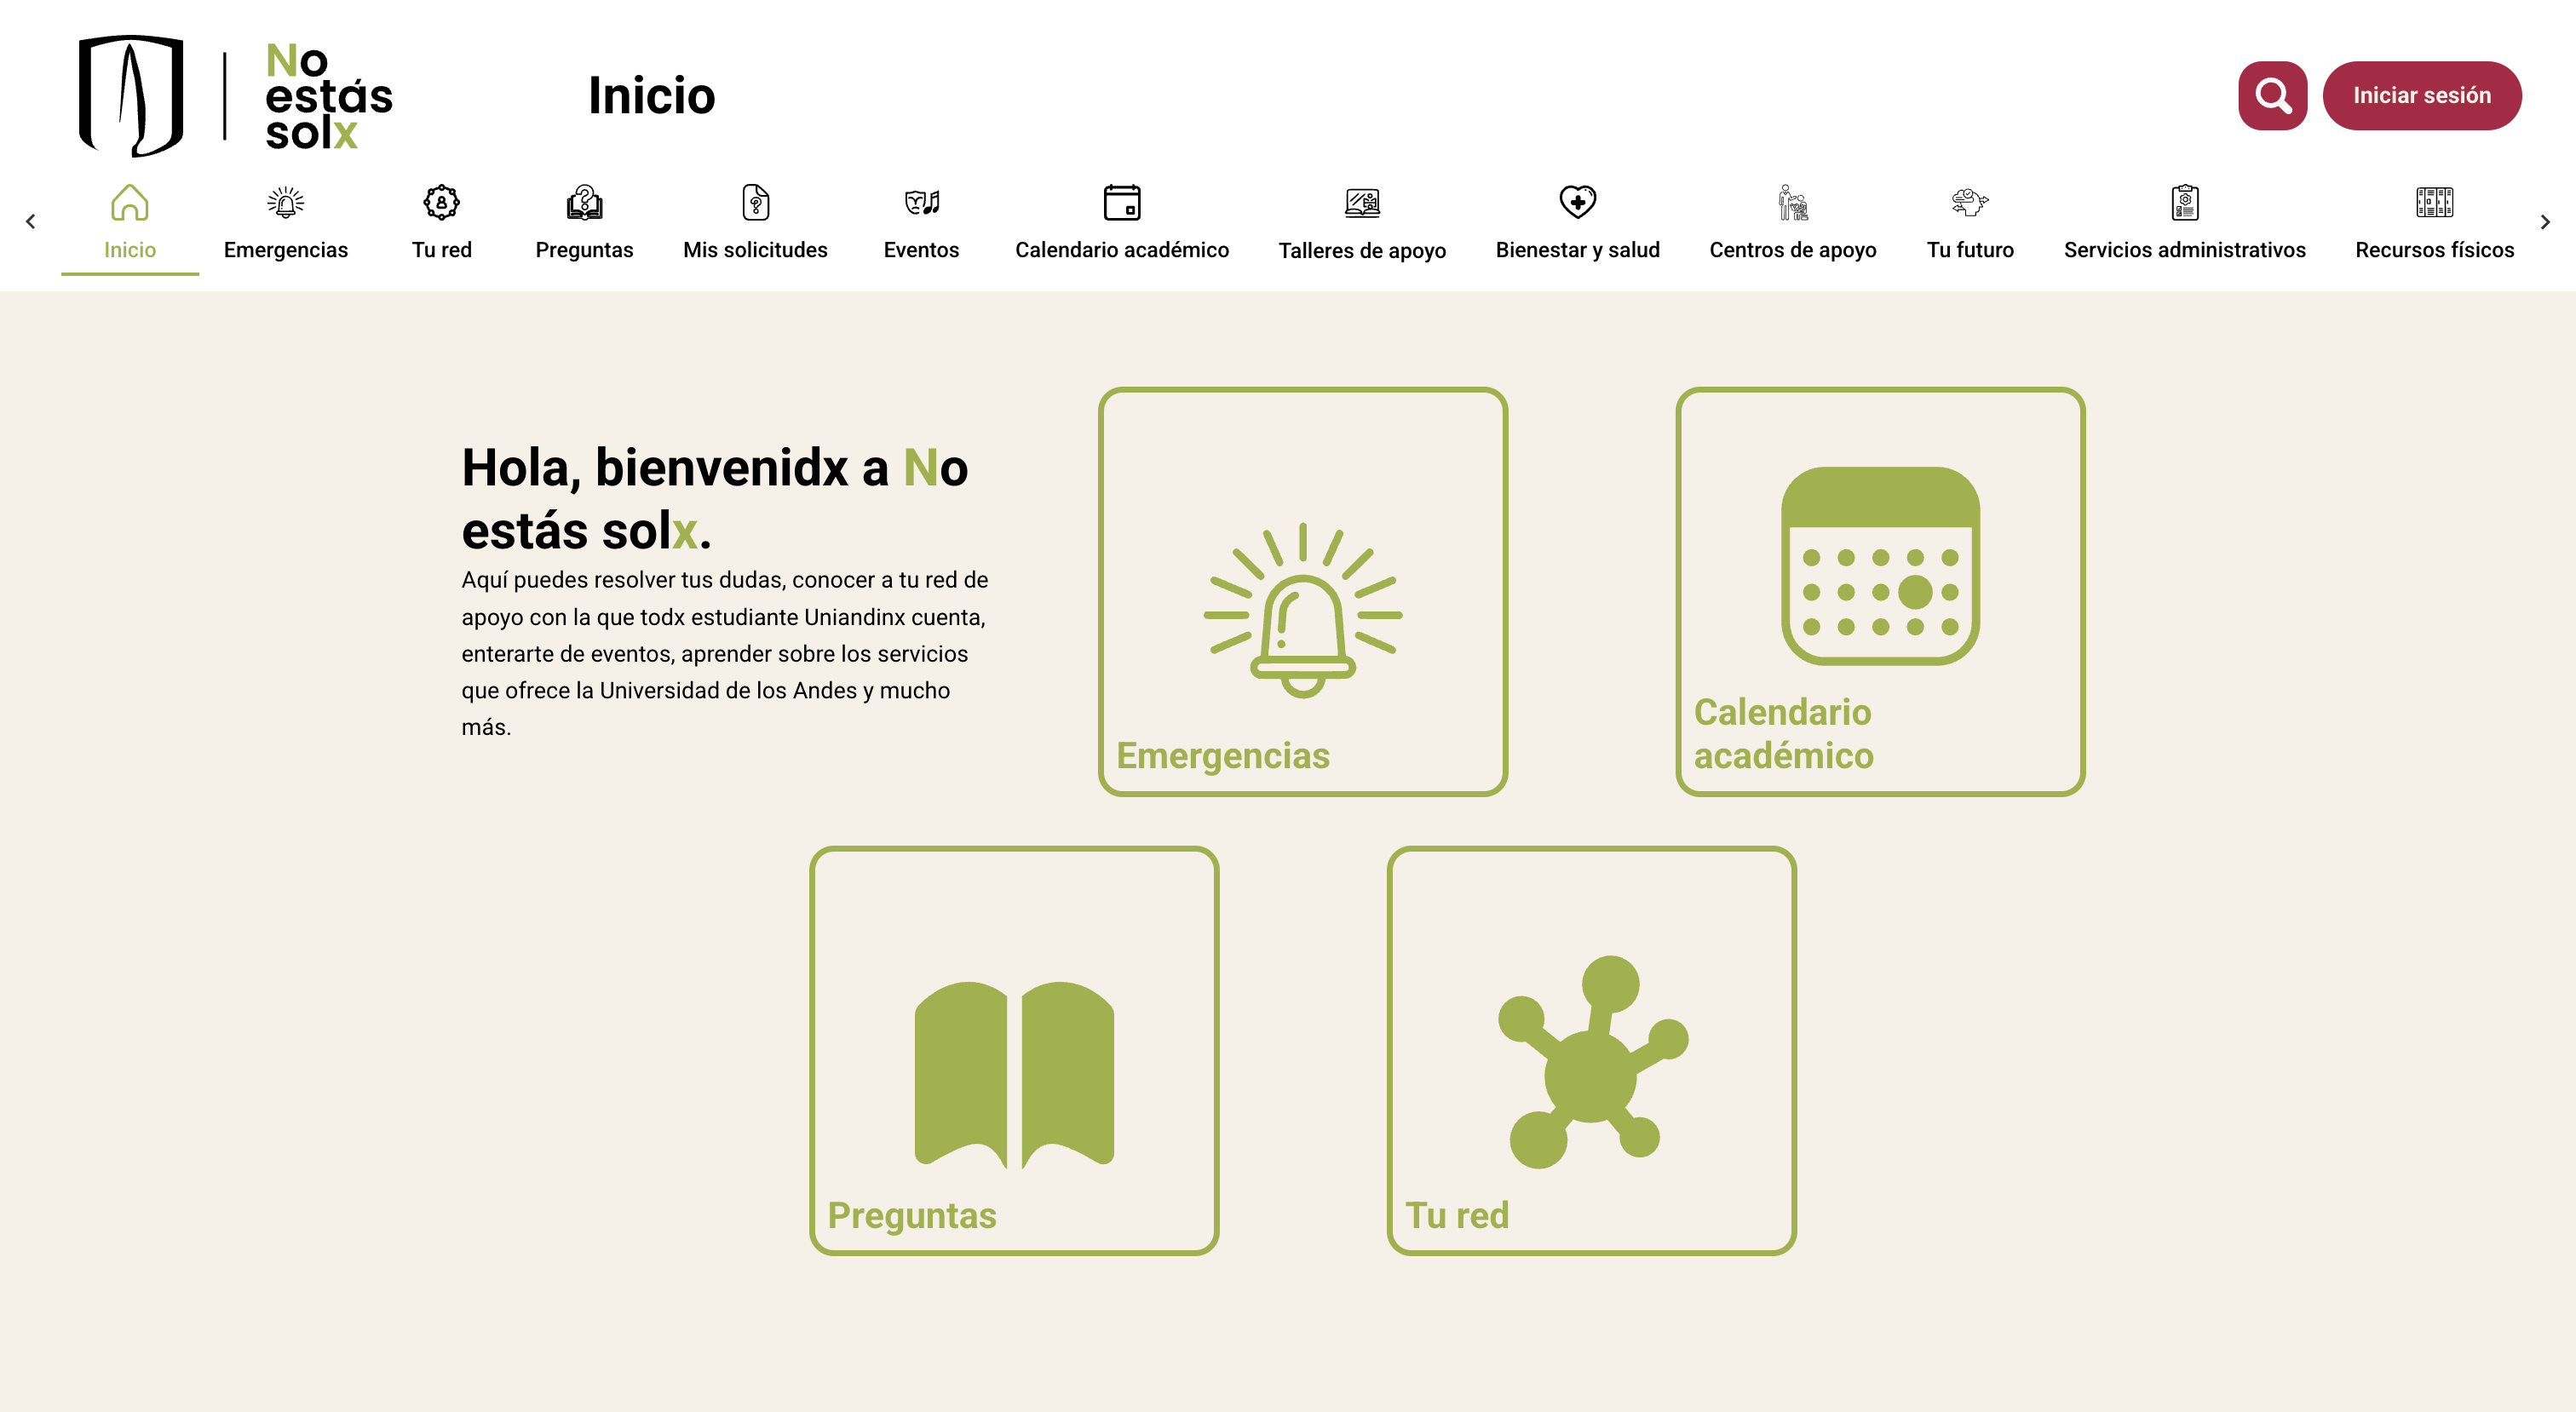
\includegraphics[width=0.8\textwidth]{assets/nes/landing.png}
	\caption{Página inicial de NES.}
	\label{fig:landing}
\end{figure}

Una vez iniciada la sesión, la página inicial de NES se transforma a la vista de estudiante, como se muestra en la figura \ref{fig:landing_estudiante}. Esa vista difiere de la anterior en tanto que ahora existe un botón adicional, titulado Mi perfil académico. Esta es la primera forma de acceder al Perfil del estudiante: pulsando el botón \textit{Mi perfil académico}.

\begin{figure}[H]
	\centering
	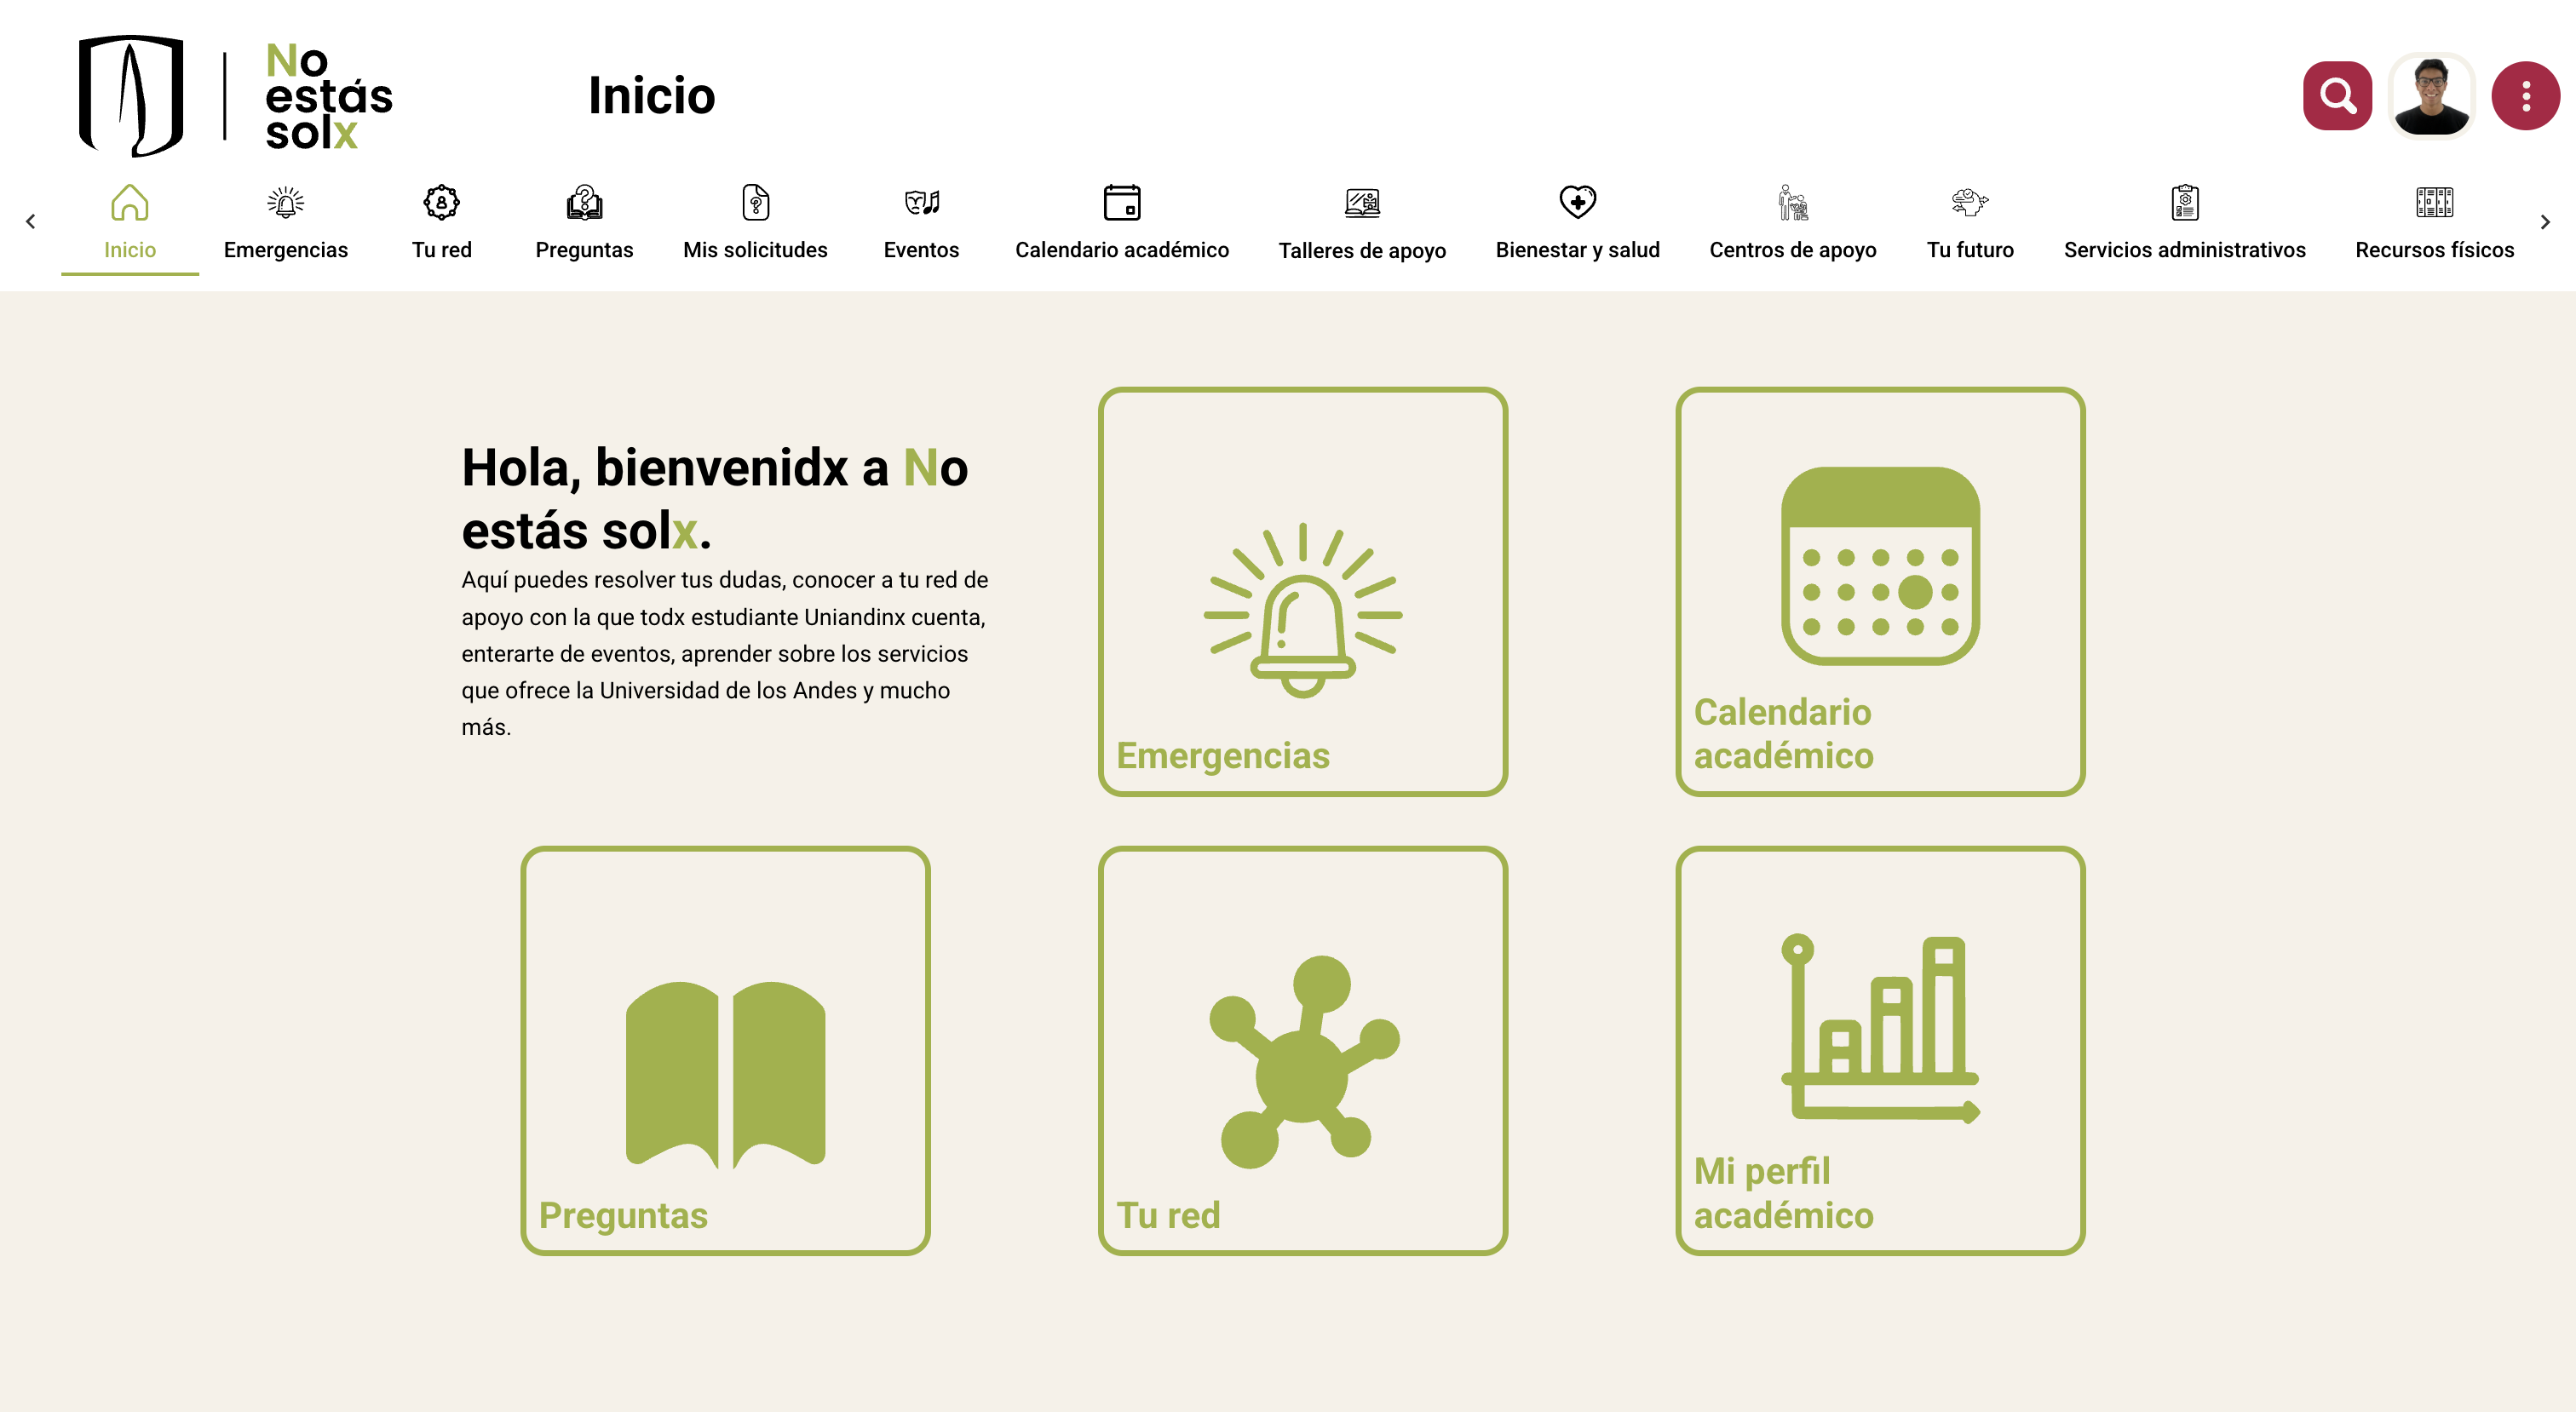
\includegraphics[width=0.8\textwidth]{assets/nes/landing_estudiante.png}
	\caption{Página inicial de NES para un estudiante.}
	\label{fig:landing_estudiante}
\end{figure}

La segunda manera de acceder al Perfil del estudiante como alumno es pulsando en su fotografía, que se ubica en la parte superior derecha de la página inicial de \gls{NES} para estudiantes. Al hacer clic en la fotografía, se despliega la ventana modal que se puede ver en la figura \ref{fig:menu_estudiante}, que incluye la opción \textit{Ver mi perfil académico}. Al pulsar en esta opción, se accede al Perfil del estudiante.

\begin{figure}[H]
	\centering
	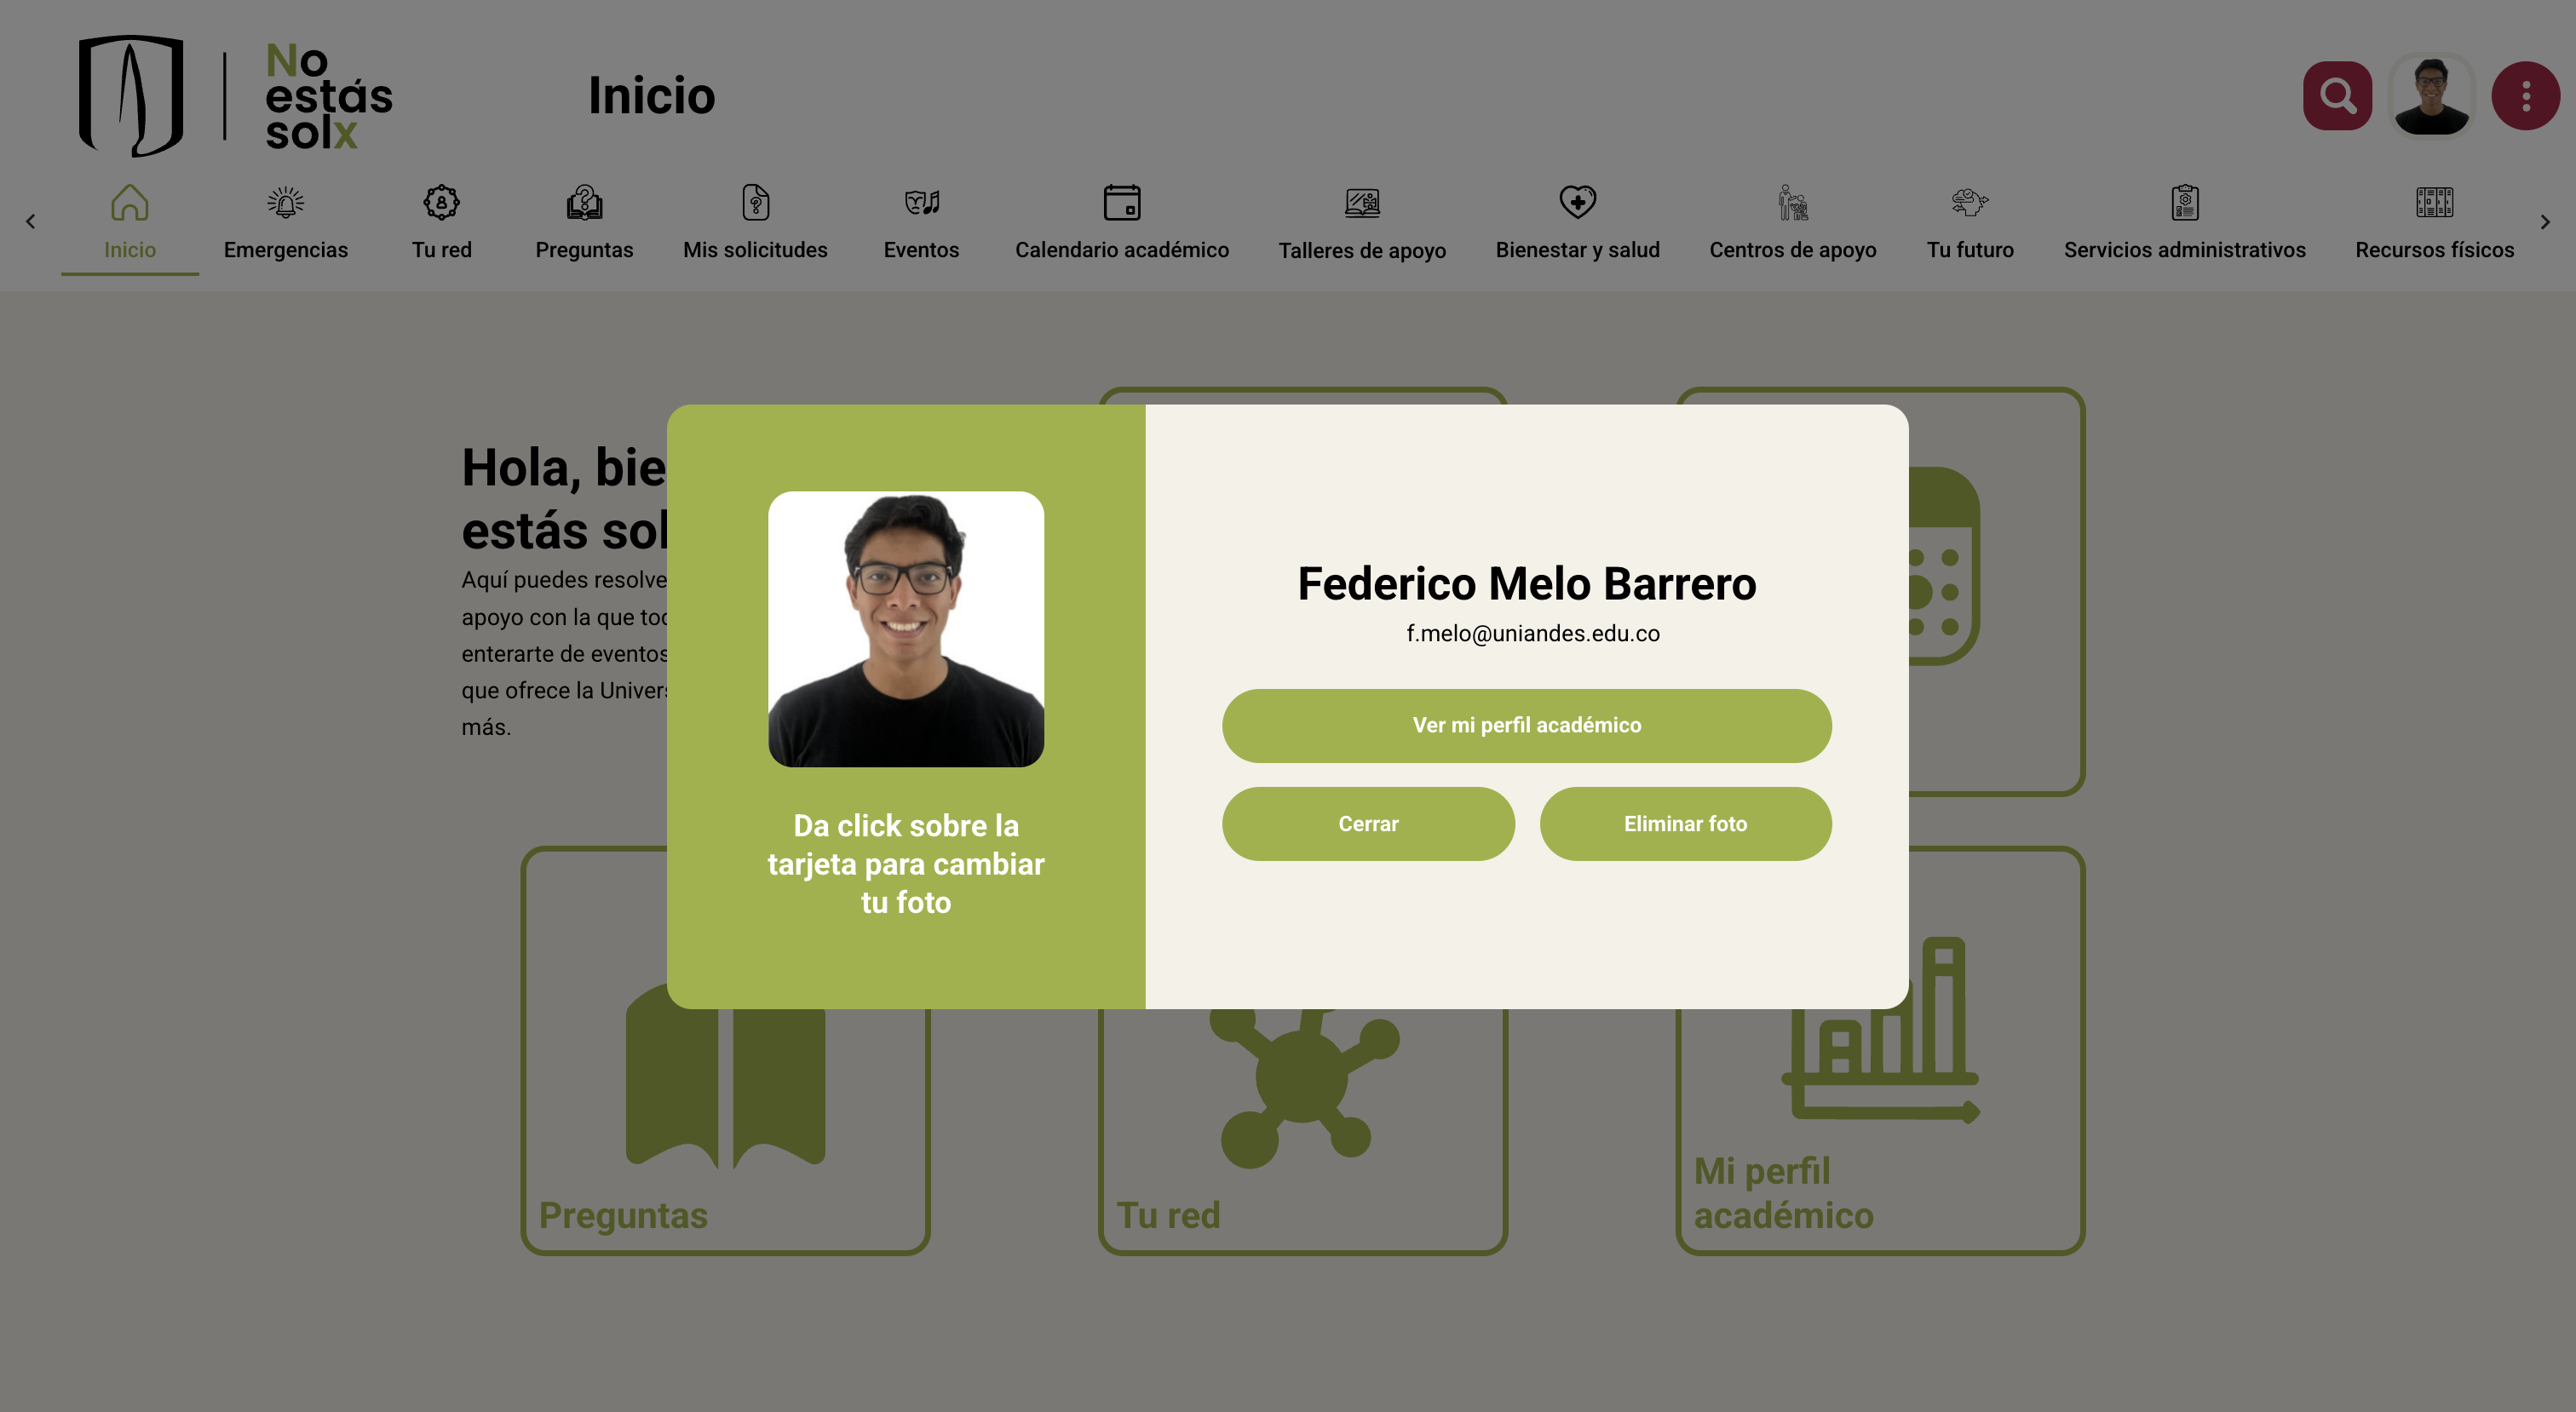
\includegraphics[width=0.8\textwidth]{assets/nes/menu_estudiante.png}
	\caption{Ventana modal de opciones para el estudiante.}
	\label{fig:menu_estudiante}
\end{figure}

\subsubsection{Acceso al Perfil del estudiante como profesor o directivo}

El acceso al perfil del estudiante como profesor o directivo difiere del acceso como alumno principalmente en el hecho de que el profesor o directivo debe seleccionar el estudiante cuyo perfil desea visualizar. Para ello, tras haber iniciado sesión en \gls{NES} con su correo Uniandes y su contraseña, debe dirigirse a la pestaña Tus aconsejados en la barra de navegación superior. Una vez seleccionada esta pestaña, se despliega una lista de estudiantes como la que se muestra en la figura \ref{fig:tus_aconsejados}.

\begin{figure}[H]
	\centering
	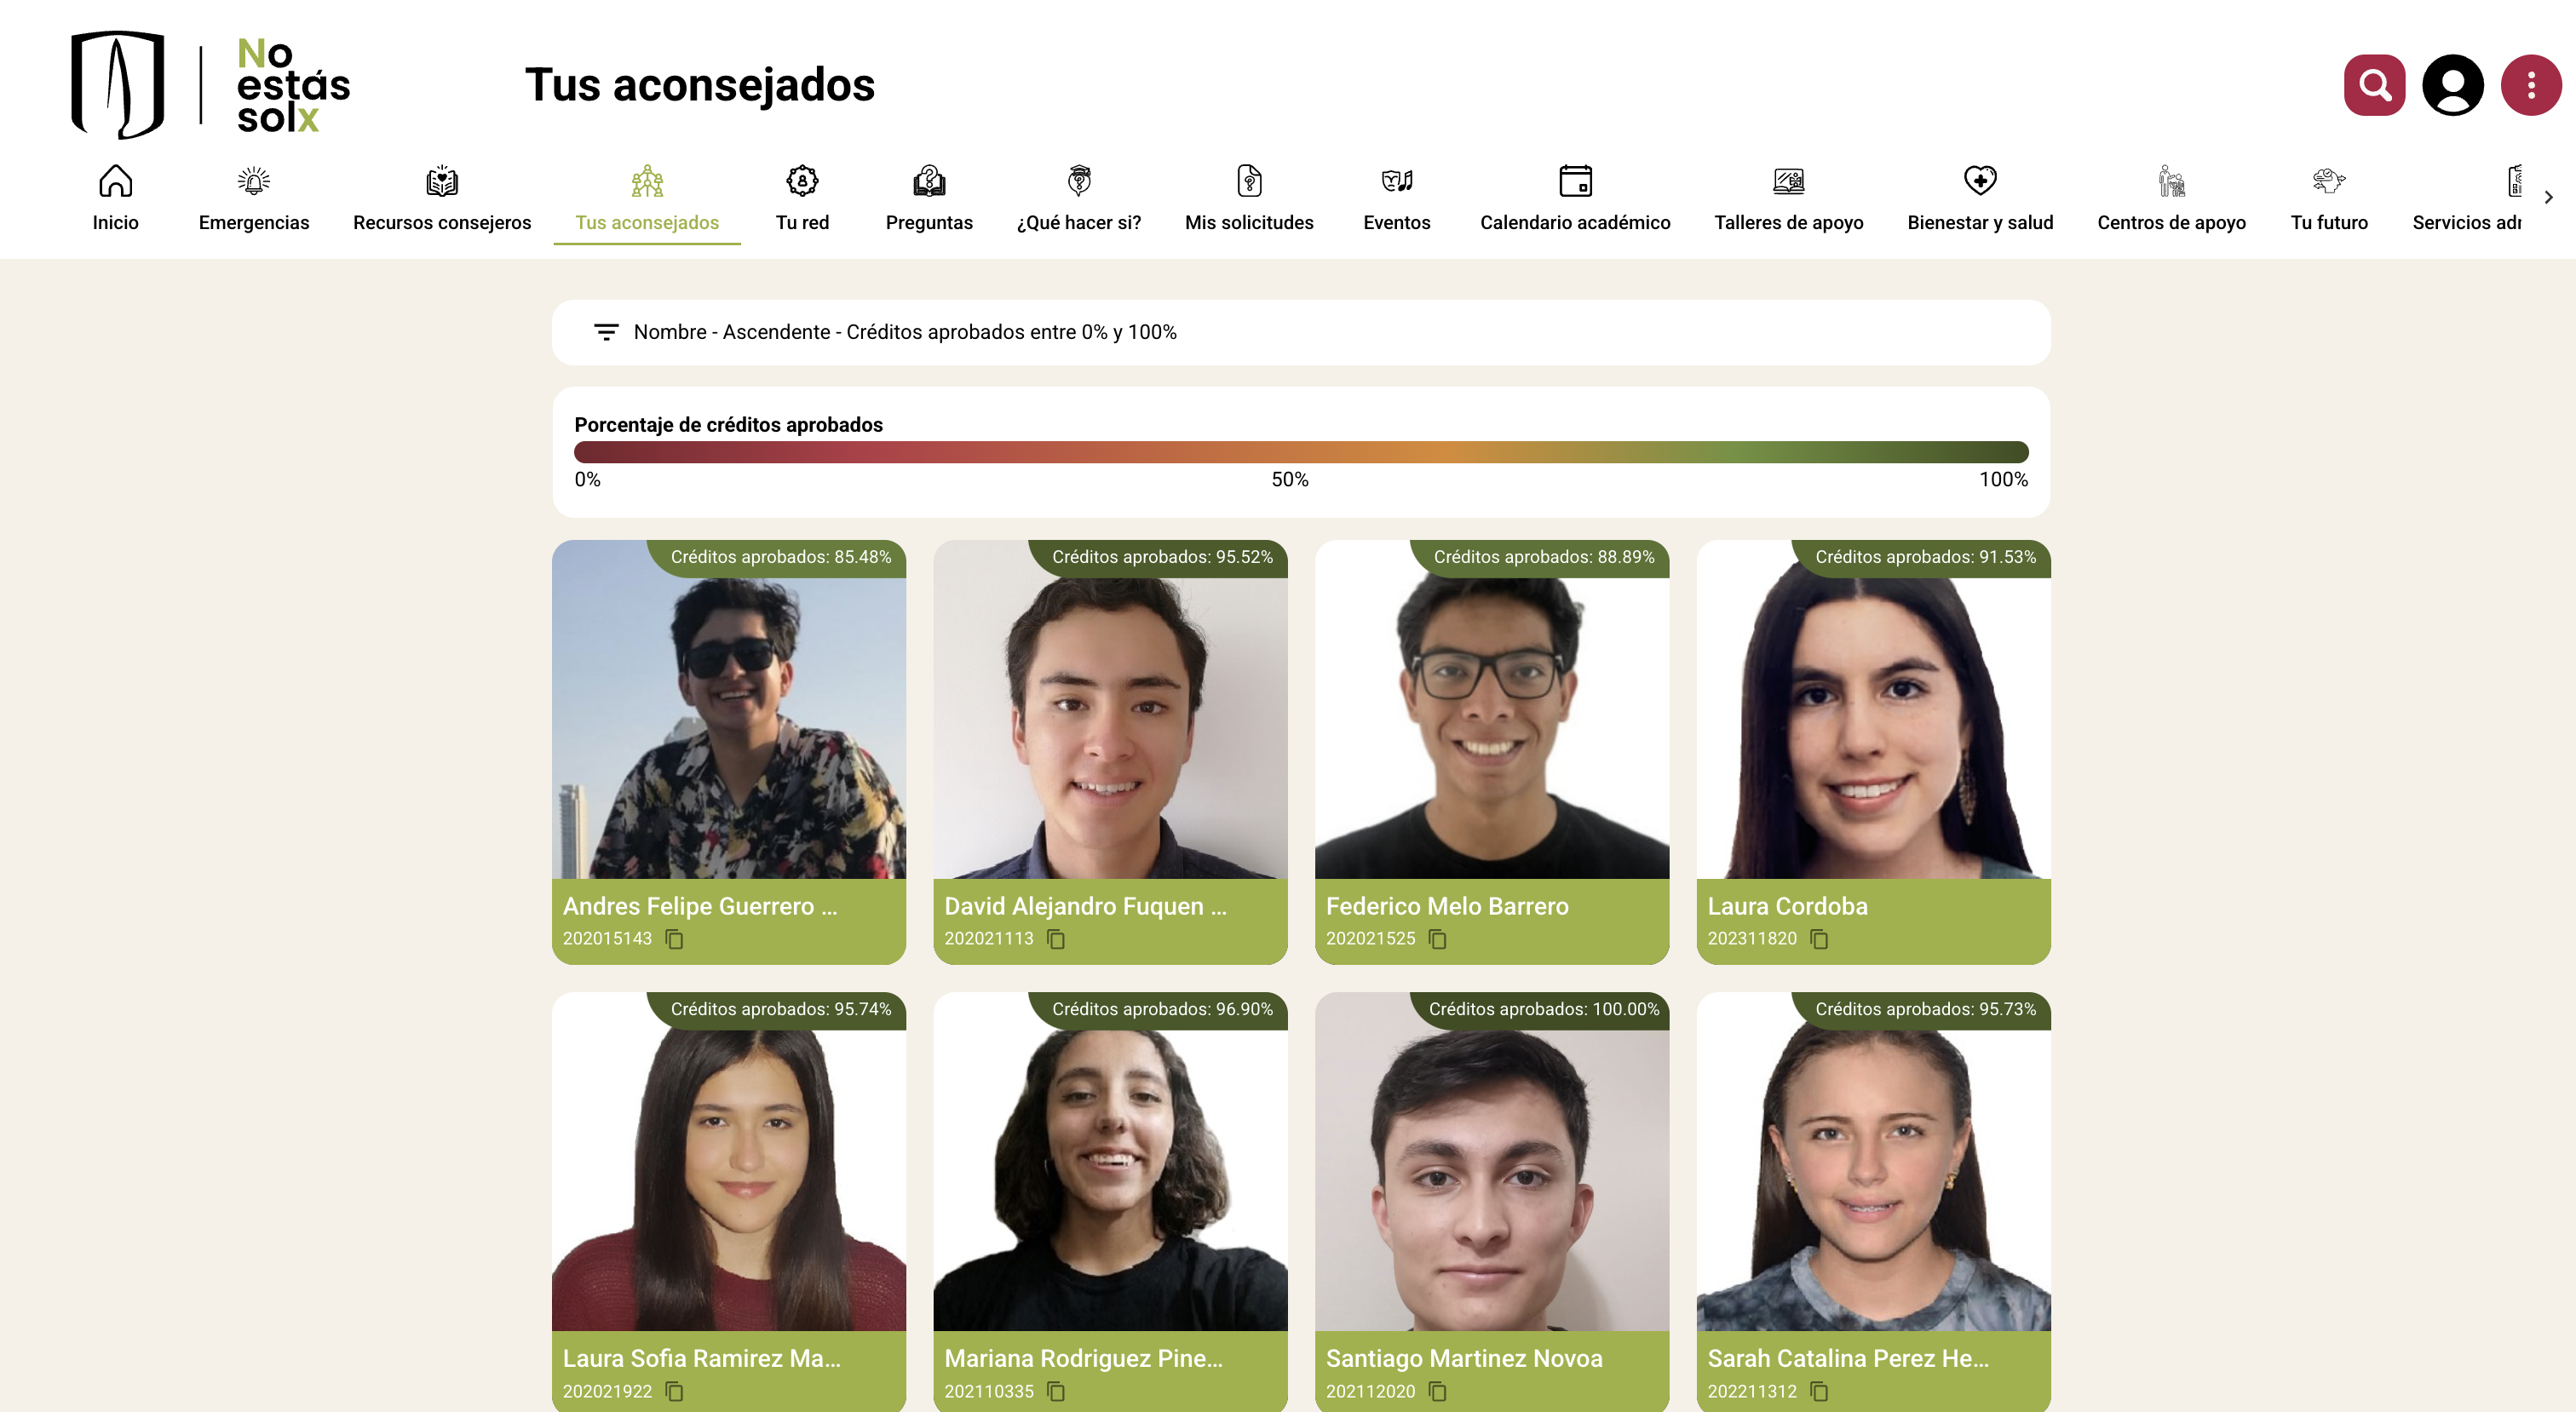
\includegraphics[width=0.8\textwidth]{assets/nes/tus_aconsejados.png}
	\caption{Pestaña Tus aconsejados en NES.}
	\label{fig:tus_aconsejados}
\end{figure}

En esta lista, el profesor o directivo puede seleccionar al alumno cuyo perfil desea visualizar. Al hacer clic sobre la tarjeta que representa a esa persona, se accede al Perfil del estudiante de ese alumno en particular. Los estudiantes que aparecen en ese listado dependen del rol del profesor o directivo en la Universidad, así como de las políticas de gobierno de datos de la Universidad. Para los profesores consejeros, la lista se limita a sus aconsejados. Dependiendo del rol del usuario en cuestión, es posible que pueda hacer uso de la barra de búsqueda en la parte superior derecha de la interfaz para buscar a cualquier estudiante de la Universidad, ya sea por su nombre, por su correo Uniandes o por su código estudiantil.

Más aún, en la pestaña Tus aconsejados, el profesor o directivo puede pulsar en el ícono de tres rayas horizontales, ubicado en la parte superior izquierda, para desplegar un menú lateral con opciones de filtrado, como se muestra en la figura \ref{fig:filtros}. Allí, es posible ordenar los alumnos mostrados por nombre o porcentaje de créditos aprobados, así como utilizar la barra deslizante para fijar un rango de porcentaje de créditos aprobados. Para algunos roles, es posible marcar la opción que permite visualizar a todos los estudiantes de la Universidad, en lugar de solo los aconsejados, con base en las políticas de gobierno de datos de la Universidad.

\begin{figure}[H]
	\centering
	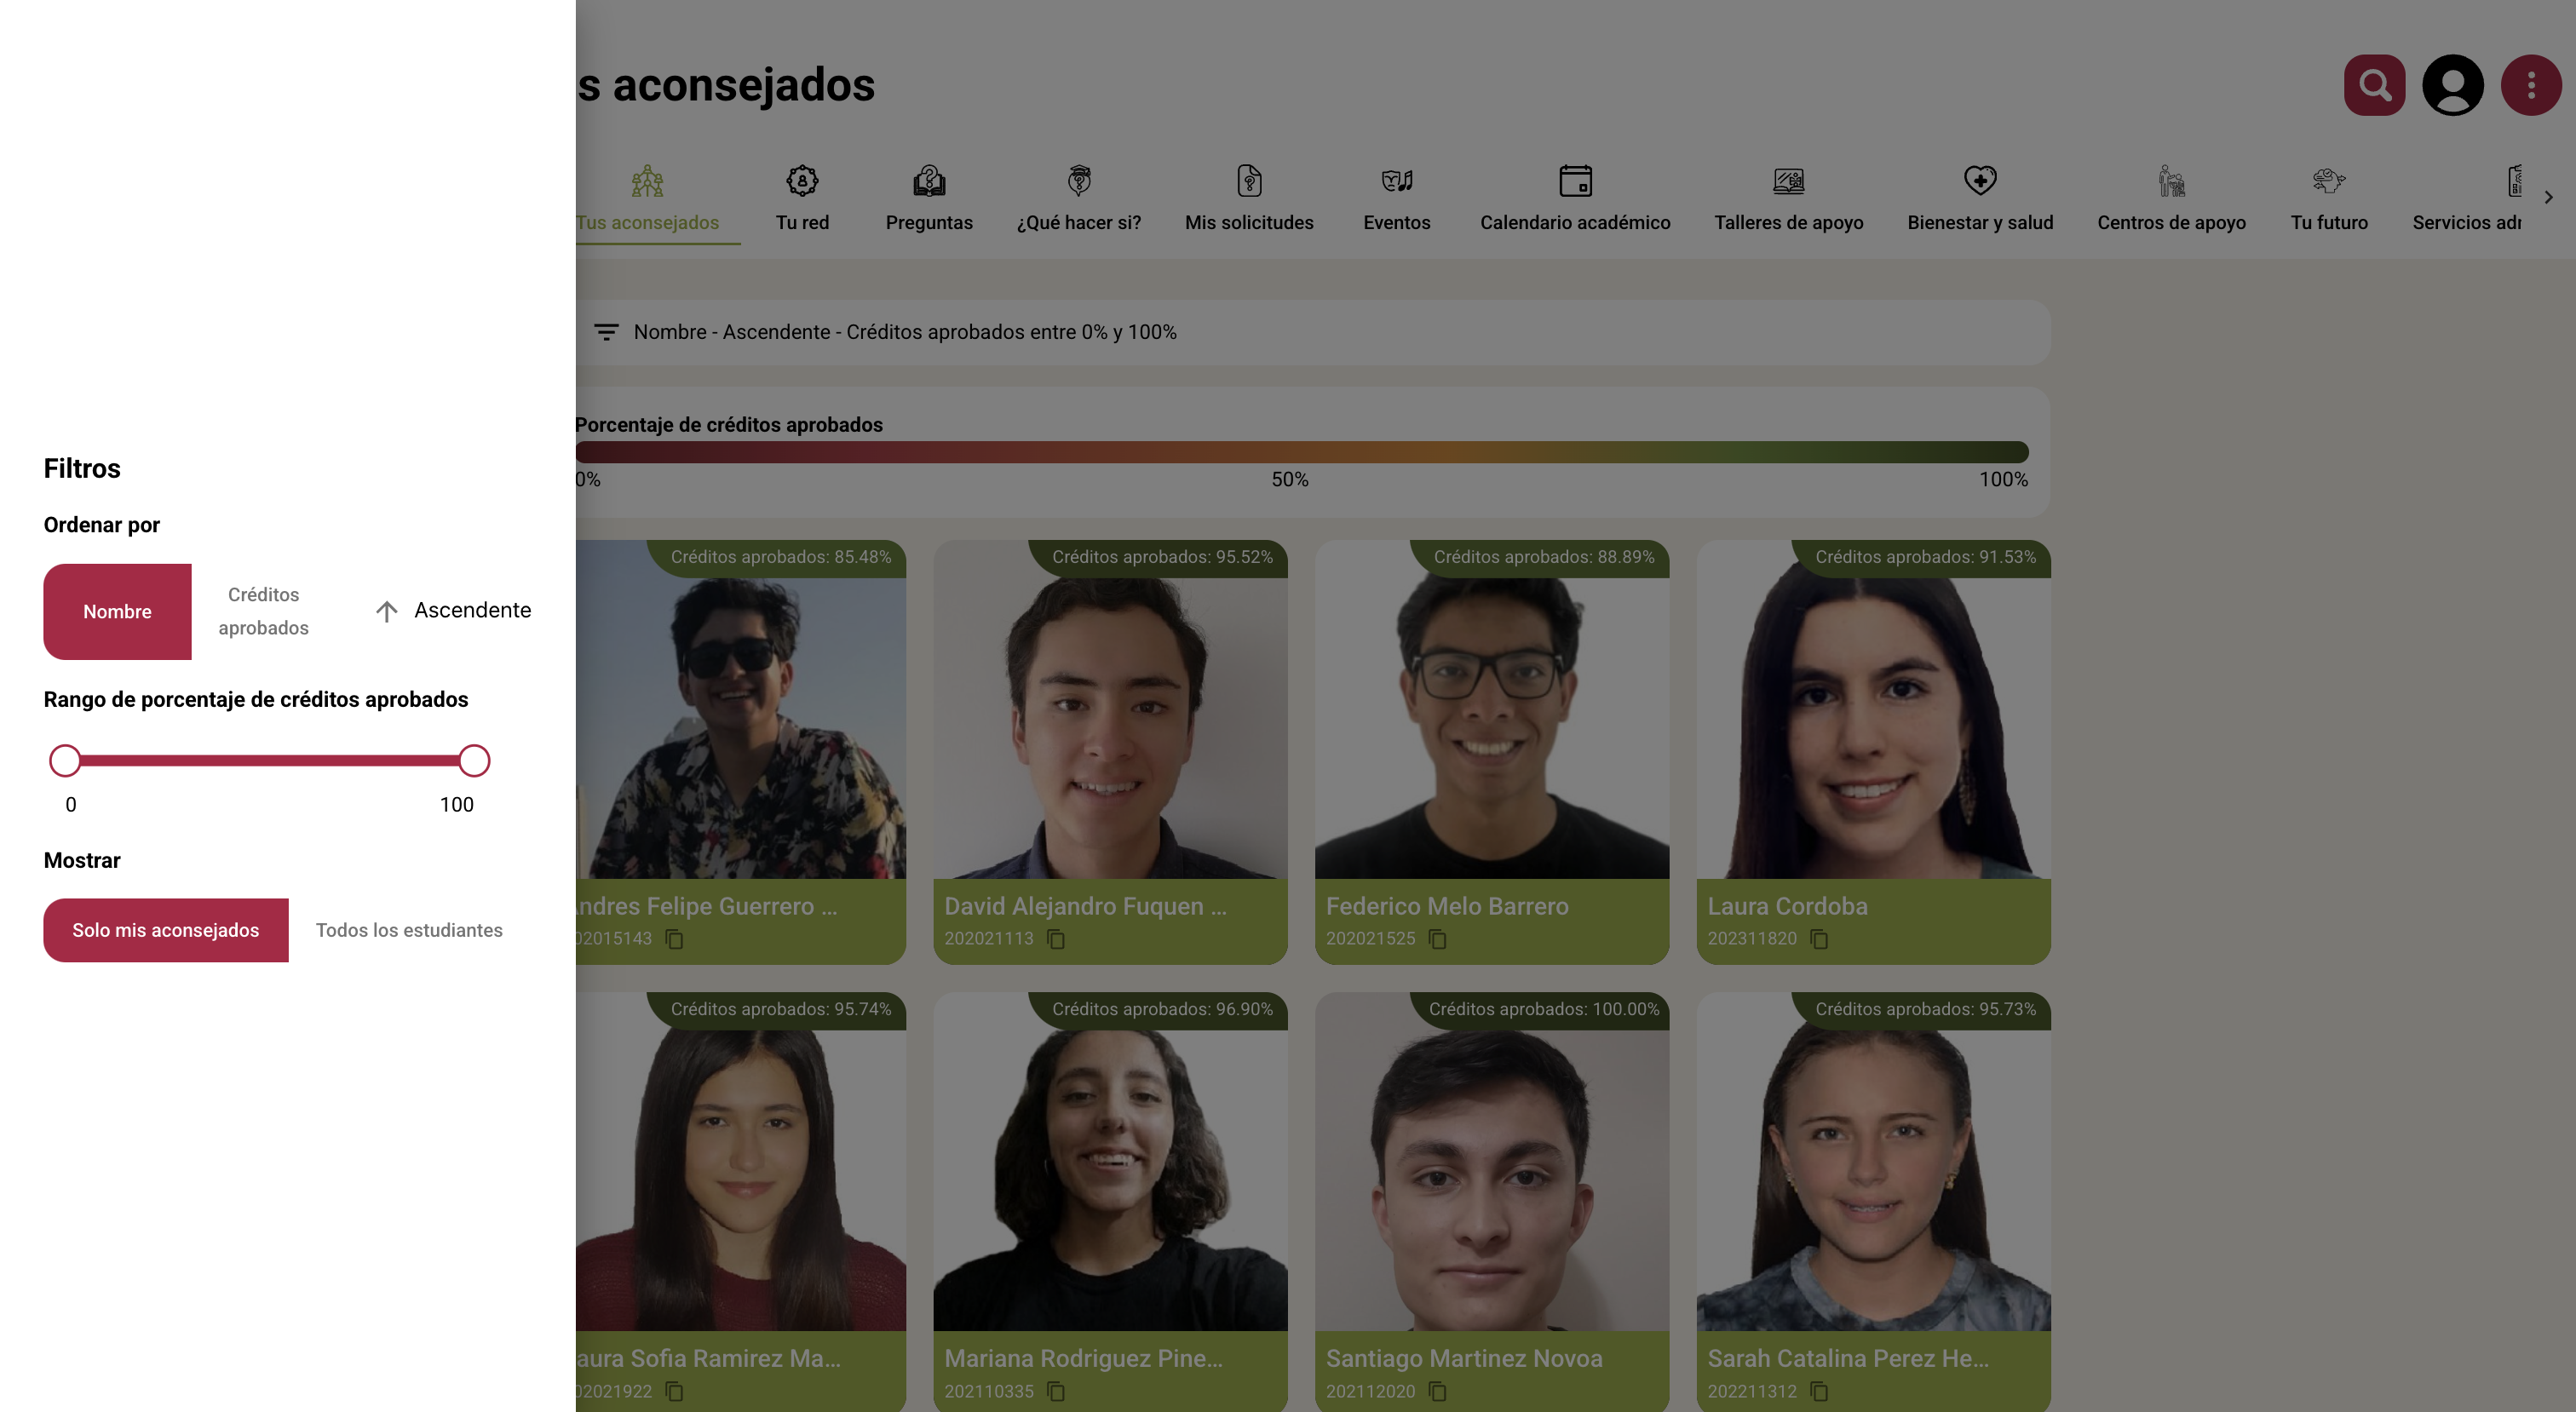
\includegraphics[width=0.8\textwidth]{assets/nes/filtros.png}
	\caption{Menú de filtros en la pestaña Tus aconsejados.}
	\label{fig:filtros}
\end{figure}

\subsection{Disposición general}

El Perfil del estudiante tiene la misma disposición general en cualquiera de sus presentaciones, independiente de si el usuario es un estudiante, un profesor o un directivo. La interfaz se divide en dos secciones principales: a la izquierda, se ubica una tarjeta con información personal del estudiante; a la derecha, se encuentra la pestaña que esté activa. La figura \ref{fig:perfil} muestra la disposición general del Perfil del estudiante con la pestaña Desempeño activa, que es la pestaña por defecto.

\begin{figure}[H]
	\centering
	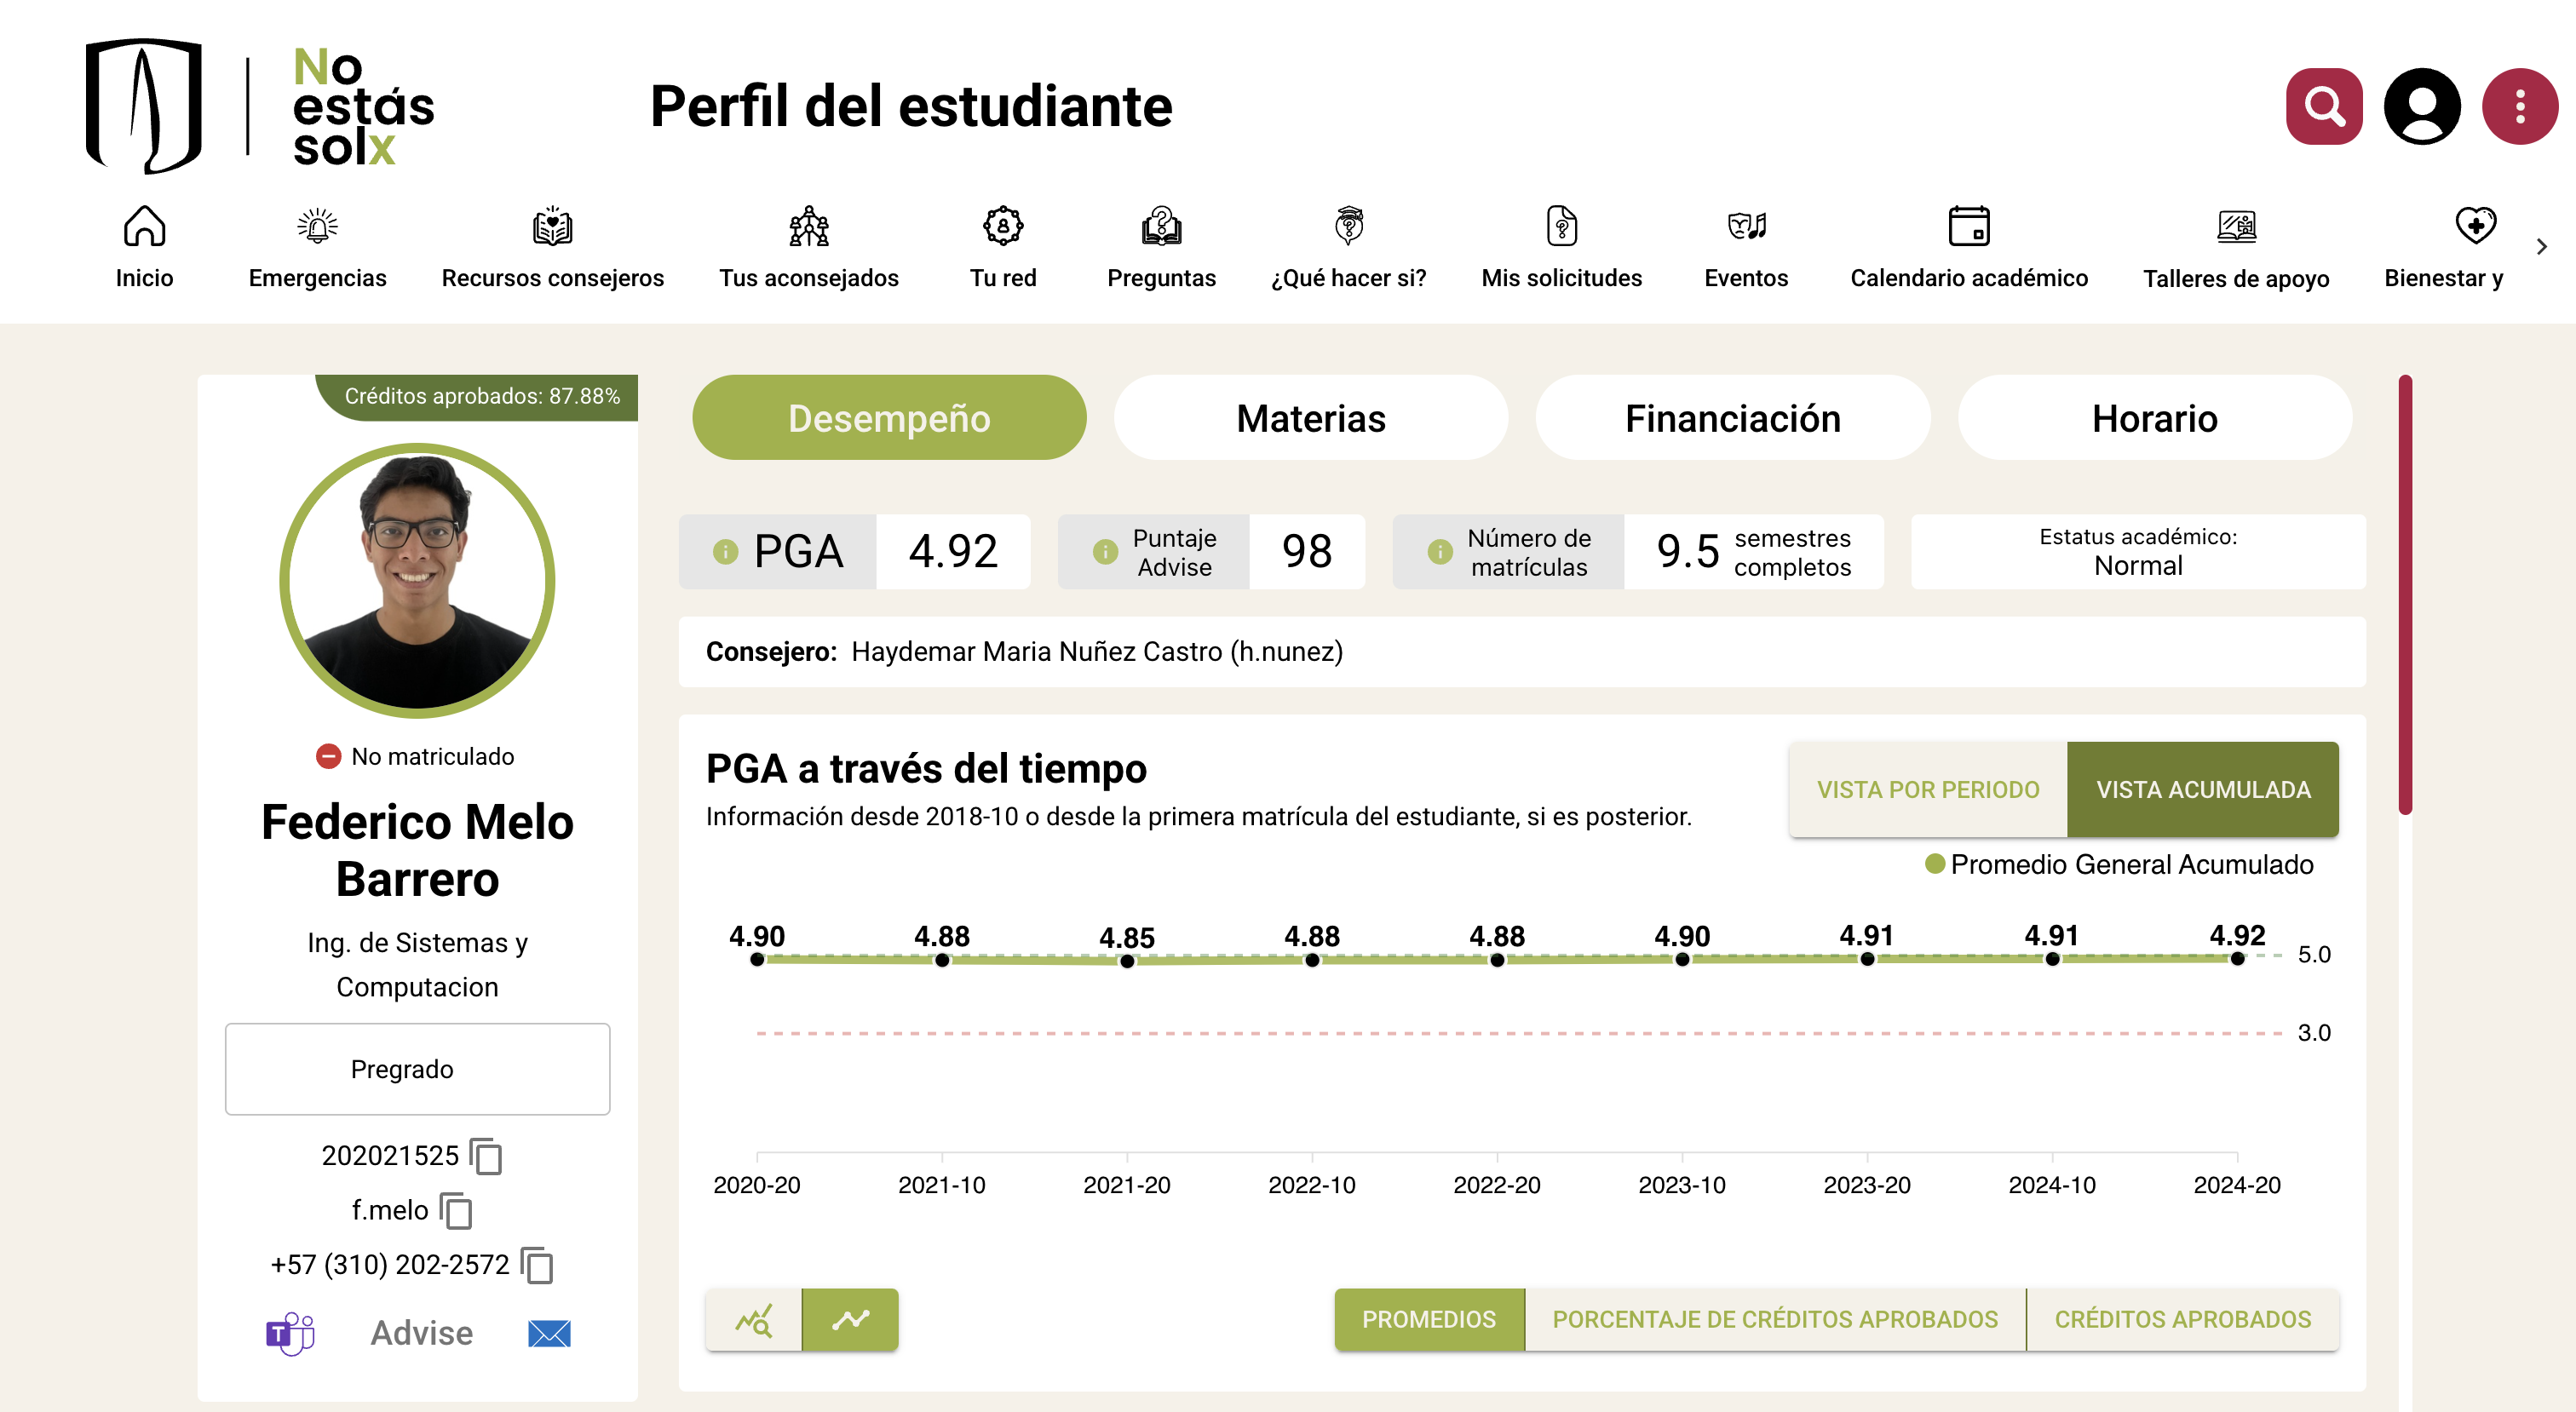
\includegraphics[width=0.8\textwidth]{assets/nes/perfil.png}
	\caption{Disposición general del Perfil del estudiante.}
	\label{fig:perfil}
\end{figure}

La sección de información personal del estudiante contiene toda la información relevante para identificarlo. En la parte superior, se presenta prominentemente la fotografía del alumno, seguida de su nombre completo y el programa académico al que pertenece.

Tras eso, se plasma su nivel académico. En caso de que el estudiante haya estado afiliado a la Universidad en distintos niveles académicos, ese componente se convierte en un selector que permite seleccionar el nivel académico que se desea visualizar, como se muestra en la figura \ref{fix:selector}. Al cambiar el nivel académico, cambia por completo el Perfil del estudiante, pues toda la información presentada en las pestañas se ajusta al nivel académico seleccionado.

\begin{figure}[H]
	\centering
	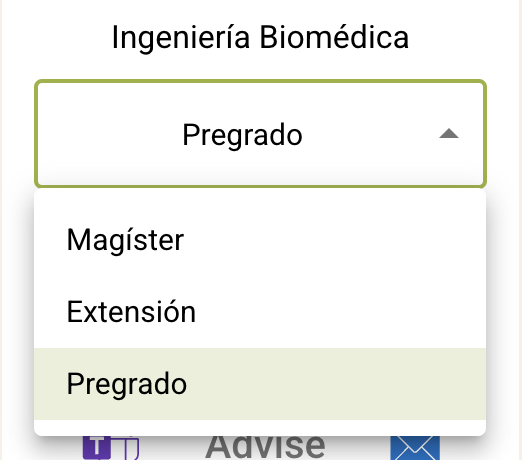
\includegraphics[width=0.4\textwidth]{assets/nes/selector.png}
	\caption{Selector de nivel académico en el perfil de un estudiante anónimo.}
	\label{fix:selector}
\end{figure}

Más abajo, se detallan datos como el código Uniandes del estudiante, su usuario de correo institucional y su número de contacto, este último solo disponible para directivos. Cada uno de esos tres datos tienen a su derecha un botón que facilita copiarlo al portapapeles. Finalmente, se ofrecen botones de interacción directa, como un enlace para asesoramiento mediante Microsoft Teams y otro para enviar correos electrónicos, lo que facilita la comunicación inmediata con el alumno.

La sección de información personal del estudiante está diseñada para que el Perfil gire en torno a la persona. Independientemente de la pestaña activa en la interfaz, los datos personales del alumno permanecen siempre visibles en la parte izquierda de la pantalla. La interfaz dispone de un sistema de scroll independiente para las dos secciones, permitiendo navegar en la pestaña seleccionada sin que se pierda de vista la información principal del estudiante. La fotografía, ubicada de forma prominente, permanece siempre visible y refuerza la conexión humana, recordando en todo momento que detrás de los datos hay una persona con identidad y contexto.

\subsection{Pestañas del Perfil del estudiante}

El Perfil del estudiante se compone de cuatro pestañas principales: Desempeño, Materias, Financiación y Horario. Los nombres de las pestañas son cortos y dicientes: la primera, Desempeño, contiene toda la información asociada al rendimiento académico; la segunda, Materias, consta de un listado exhaustivo de todas las materias inscritas; la tercera, Financiación, presenta información detallada sobre cómo el estudiante ha financiado sus estudios; y la cuarta, Horario, muestra el horario de clases del alumno al momento de la consulta.

Cada una de estas pestañas presenta información relevante para el estudiante, el profesor o el directivo, dependiendo del rol del usuario que accede al Perfil. A continuación, se dedica una sección a cada una de las pestañas, describiendo la información presentada y las funcionalidades disponibles.

\subsubsection{Pestaña de Desempeño}

La pestaña de Desempeño es la pestaña por defecto que se muestra al acceder al Perfil del estudiante. Esta pestaña ofrece un análisis detallado del rendimiento académico a través del tiempo. A continuación, se detallan uno a uno los elementos que componen la pestaña de Desempeño. Para empezar, la figura \ref{fig:desempeno} presenta un primer pedazo de la pestaña de Desempeño, que contiene los indicadores claves y la gráfica central.

\begin{figure}[H]
	\centering
	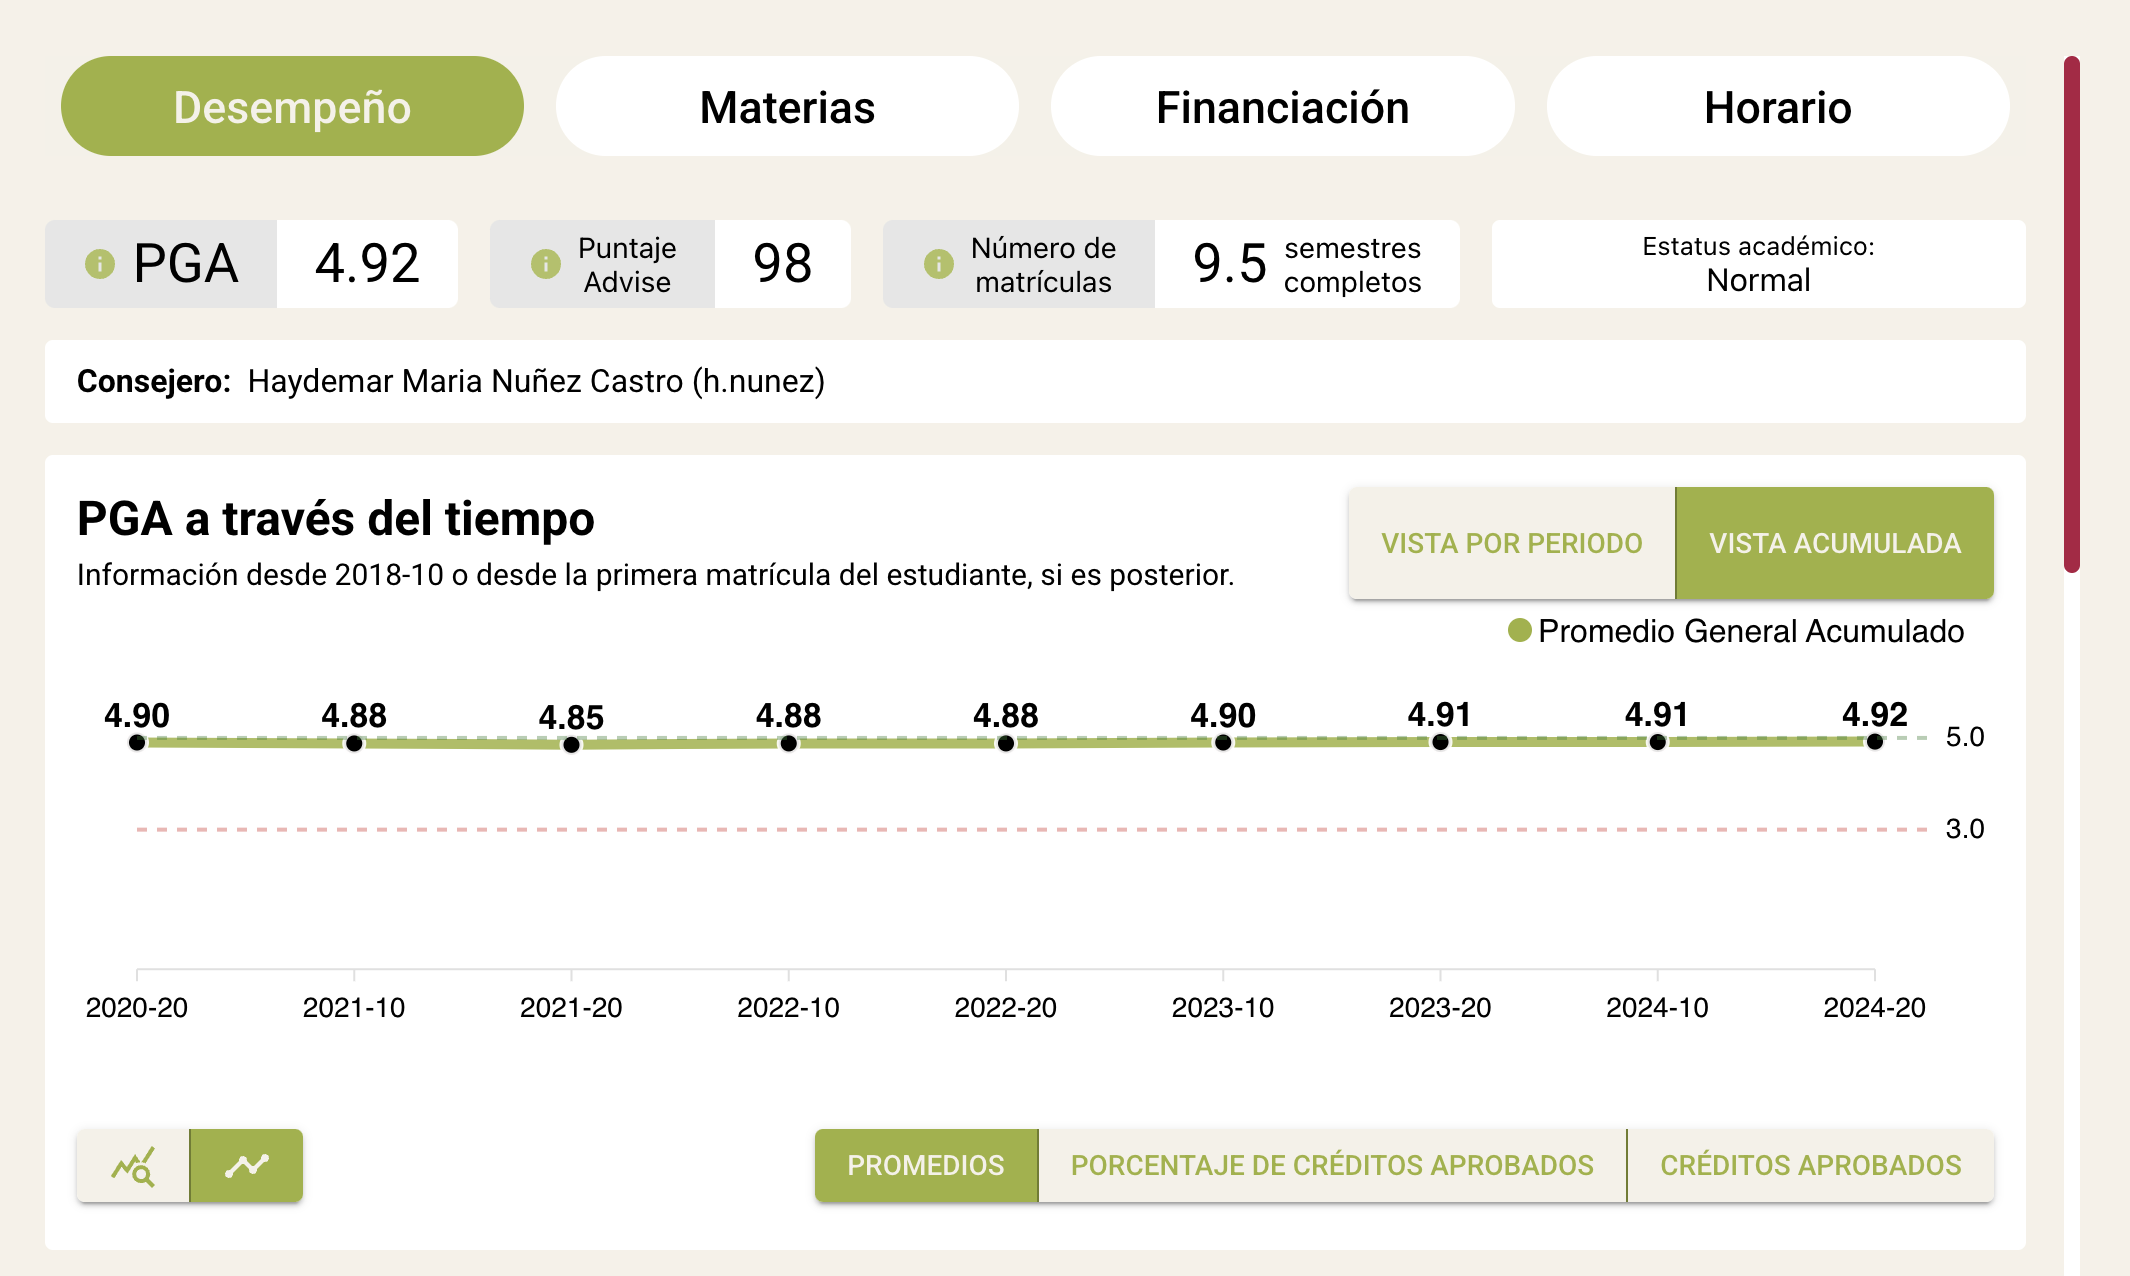
\includegraphics[width=0.8\textwidth]{assets/nes/desempeno_1.png}
	\caption{Parte de arriba de la pestaña de Desempeño.}
	\label{fig:desempeno}
\end{figure}

\paragraph{Indicadores clave} En la parte superior de la pestaña, se encuentran cuatro indicadores clave que resumen el desempeño académico: el Promedio General Acumulado (PGA), el Puntaje Advise, el número de matrículas que ha realizado y el estado académico actual del estudiante.
\begin{itemize}
	\item El PGA es el principal indicador de rendimiento académico en la Universidad. De acuerdo con el Reglamento general de estudiantes de pregrado de la Universidad de los Andes, el PGA resulta de multiplicar el número de créditos de cada materia por la calificación obtenida, sumando estos productos y dividiendo el resultado por el número total de créditos calificados numéricamente.
	      % TODO: Cita
	      Su menor valor es 1.5 y su máximo valor es 5.0. El PGA se presenta con dos decimales.
	\item El Puntaje Advise es un indicador de la probabilidad de éxito académico del estudiante en la Universidad. Es calculado y provisto por la herramienta de análisis predictivo Advise y oscila entre 0 y 100. Se presenta el puntaje Advise tal y como se extrae de la herramienta.
	\item El número de matrículas representa la cantidad de semestres completos que han sido pagados y matriculados. Puede ser un número decimal, en caso de que el alumno haya cursado matrículas parciales. En esta medida, un semestre completo se valora como una matrícula; media matrícula se valora como 0.5 matrículas; y un cuarto de matrícula, un periodo intersemestral o una práctica académica se valora como 0.25 matrículas. Esta medida es un buen reflejo de la inversión realizada en la educación del estudiante.
	\item El estado académico actual del alumno es un término que resume su situación académica. [Falta descripción del estado académico.]
	      % TODO: Posibles valores del estado académico.
\end{itemize}

Estos indicadores son la primera pieza de información que el usuario ve al acceder al Perfil del estudiante y le permiten tener una visión general de su rendimiento de un vistazo. Al pasar el cursor sobre cada uno de los indicadores, se despliega una descripción detallada del indicador, que facilita su interpretación. Un ejemplo de esto se presenta en la figura \ref{fig:indicadores}, en la que se pasa el cursor por encima del indicador de Puntaje Advise.

\begin{figure}[H]
	\centering
	
\includegraphics[width=0.8\textwidth]{assets/nes/indicadores.png}
	\caption{Descripción del indicador de Puntaje Advise al pasar el cursor sobre él.}
	\label{fig:indicadores}
\end{figure}

\paragraph{Profesor consejero} Inmediatamente debajo de los indicadores clave, se muestra el nombre del consejero académico asignado al alumno. El consejero académico es un profesor de la Universidad, comisionado para asesorar a la persona en temas académicos y administrativos, y que puede ser contactado por ella en caso de necesitar orientación. A los estudiantes que cursan múltiples programas académicos se les asigna un consejero académico por cada programa. El raciocinio detrás de mostrar el consejero académico en una posición tan prominente de la pestaña radica en responsabilizar al consejero académico de la orientación del aconsejado y de su rendimiento académico, en particular cuando este ingrese a visualizar el Perfil del estudiante.

\paragraph{Gráfica central} A continuación, se encuentra una gráfica interactiva. Esta gráfica es la pieza central de la pestaña de Desempeño y realmente podría desglosarse en doce gráficas distintas. La interactividad de la gráfica es lo que permite que pueda tener muchas presentaciones distintas sin resultar abrumadora. Para explicar la gráfica, en primer lugar se listan las opciones de interacción que esta ofrece y tras eso se listan las 12 visualizaciones distintas que puede presentar al elegir determinadas opciones de interacción.

Respecto a las opciones de interacción, para variar entre las presentaciones de la gráfica, se presentan tres grupos de botones:
\begin{itemize}
	\item En la parte inferior derecha de la gráfica, se encuentra un botón que permite seleccionar la información que la gráfica despliega. Las posibles opciones son: Promedios, Porcentaje de Créditos Aprobados y Créditos Aprobados.
	\item En la parte superior derecha, se encuentra un botón que permite alternar entre la Vista por periodo y la Vista acumulada.
	\item En la parte inferior izquierda, se encuentra un botón que permite alternar entre dos escalas de la gráfica: la escala estándar, que depende del tipo de información seleccionada, y la escala relativa, que facilita la visualización del comportamiento de la información a través del tiempo.
\end{itemize}

Cada combinación de botones seleccionada resulta en una visualización distinta de la gráfica. A continuación, se listan las 12 visualizaciones distintas que puede presentar la gráfica:
\begin{enumerate}
	\item \textbf{Promedios, Vista acumulada, Escala estándar.} Esta visualización se titula \say{PGA a través del tiempo} y muestra la evolución del Promedio General Acumulado (PGA) del estudiante a lo largo del tiempo, en una escala estándar cuyo valor mínimo es 1.5 y cuyo valor máximo es 5.0. Cada punto de la gráfica representa el PGA del estudiante en un periodo académico específico. En la escala estándar se dibujan dos líneas de referencia: la inferior corresponde al PGA mínimo y se traza en rojo a la altura del 3.0; la superior corresponde al PGA máximo y se traza en verde a la altura del 5.0. Se presenta en la figura \ref{fig:pga_estandar}.

	      \begin{figure}[H]
		      \centering
		      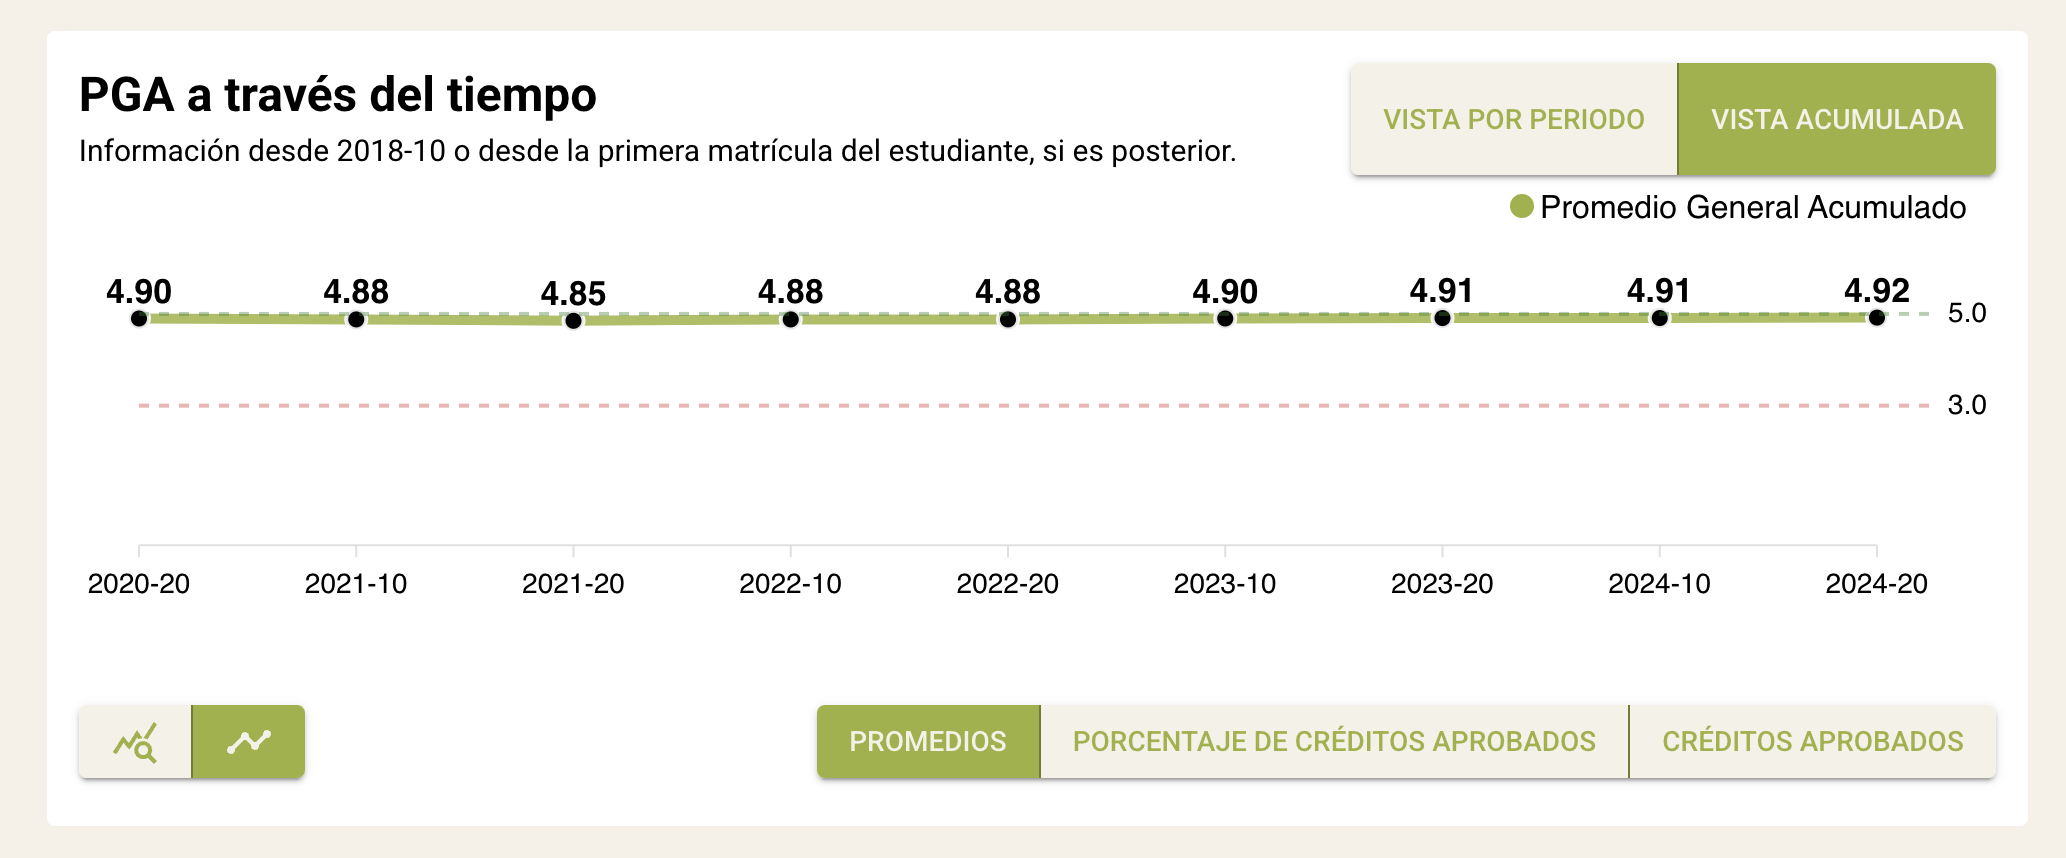
\includegraphics[width=0.8\textwidth]{assets/nes/pga_estandar.png}
		      \caption{Visualización de PGA a través del tiempo en escala estándar.}
		      \label{fig:pga_estandar}
	      \end{figure}

	\item \textbf{Promedios, Vista acumulada, Escala relativa.} Esta visualización transmite la misma información que la anterior y se titula igual. La diferencia radica en el enfoque que da a la información. Se modifica la escala de la gráfica para que el menor valor sea el PGA mínimo que el estudiante ha obtenido y el mayor valor sea el PGA máximo que ha alcanzado. Esto pone el énfasis en la variabilidad del PGA del alumno a lo largo del tiempo, permitiendo ver los periodos en los que mejoró o empeoró su rendimiento académico. Se presenta en la figura \ref{fig:pga_relativo}.

	      \begin{figure}[H]
		      \centering
		      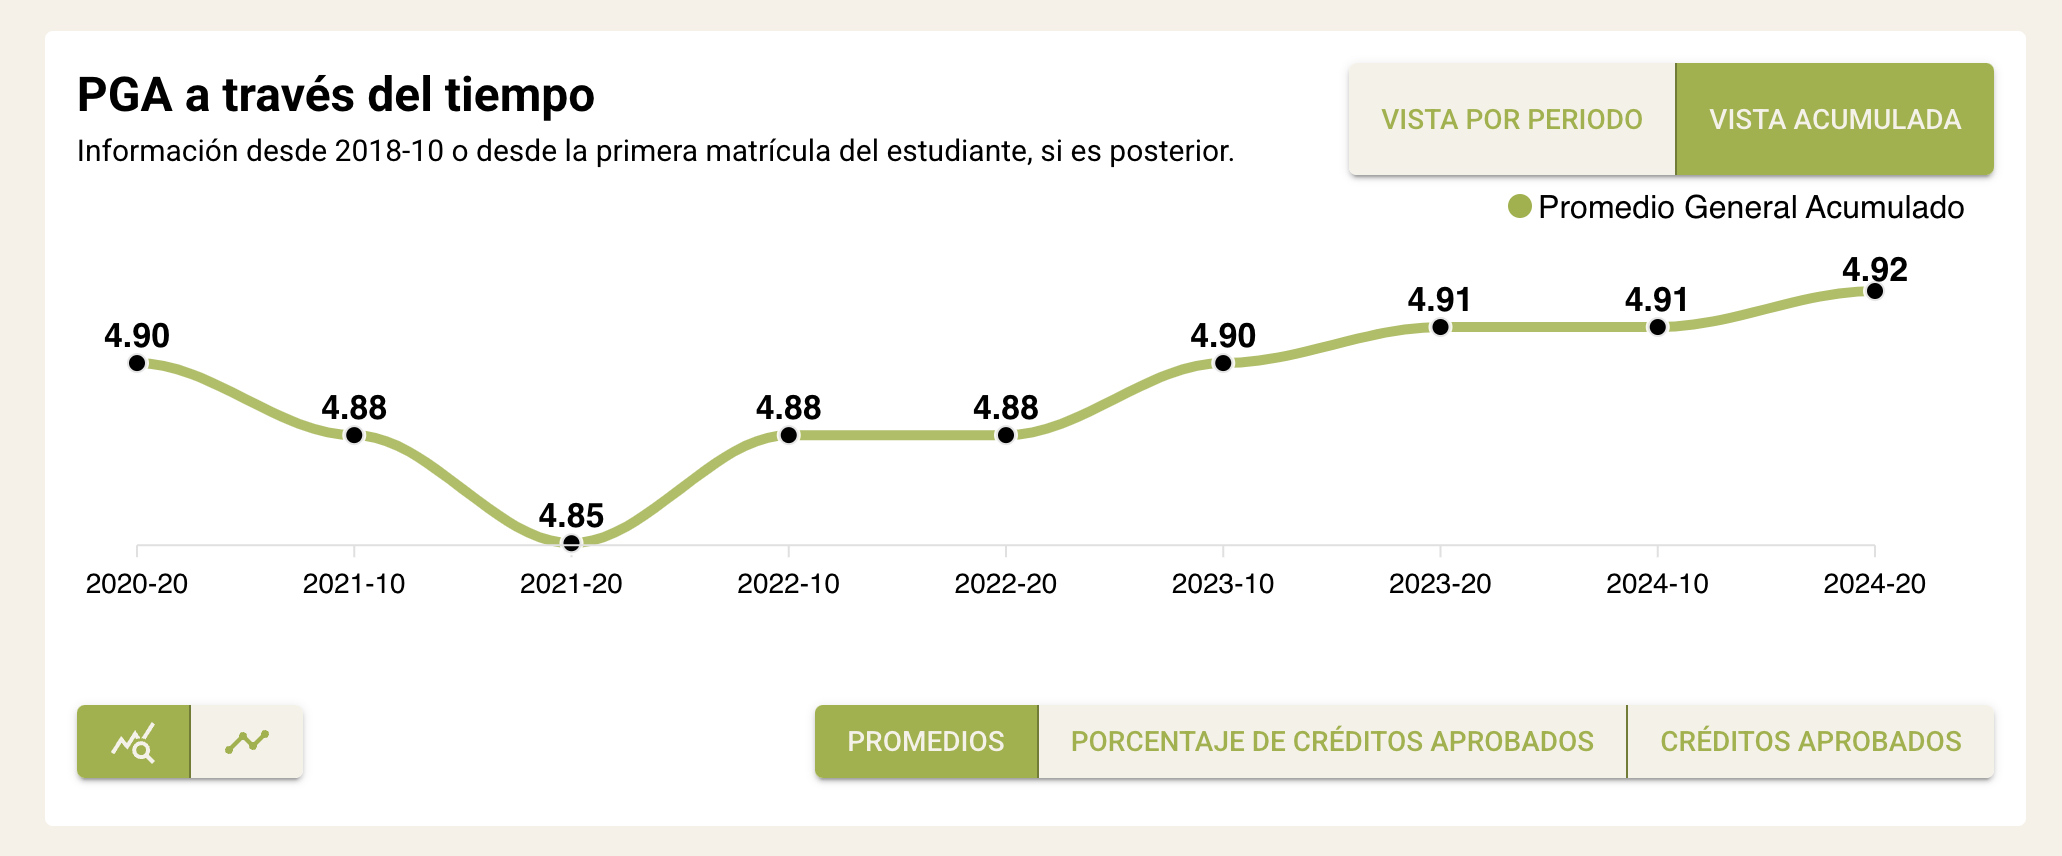
\includegraphics[width=0.8\textwidth]{assets/nes/pga_relativo.png}
		      \caption{Visualización de PGA a través del tiempo en escala relativa.}
		      \label{fig:pga_relativo}
	      \end{figure}

	\item \textbf{Promedios, Vista por periodo, Escala estándar.} Esta visualización se titula \say{Promedios semestrales a través del tiempo} y muestra los promedios semestrales que el estudiante ha obtenido a lo largo del tiempo. Cada punto de la gráfica representa el promedio semestral del alumno en un periodo académico específico. Se utiliza la misma escala estándar que en la visualización 1. Se presenta en la figura \ref{fig:promedios_estandar}.

	      \begin{figure}[H]
		      \centering
		      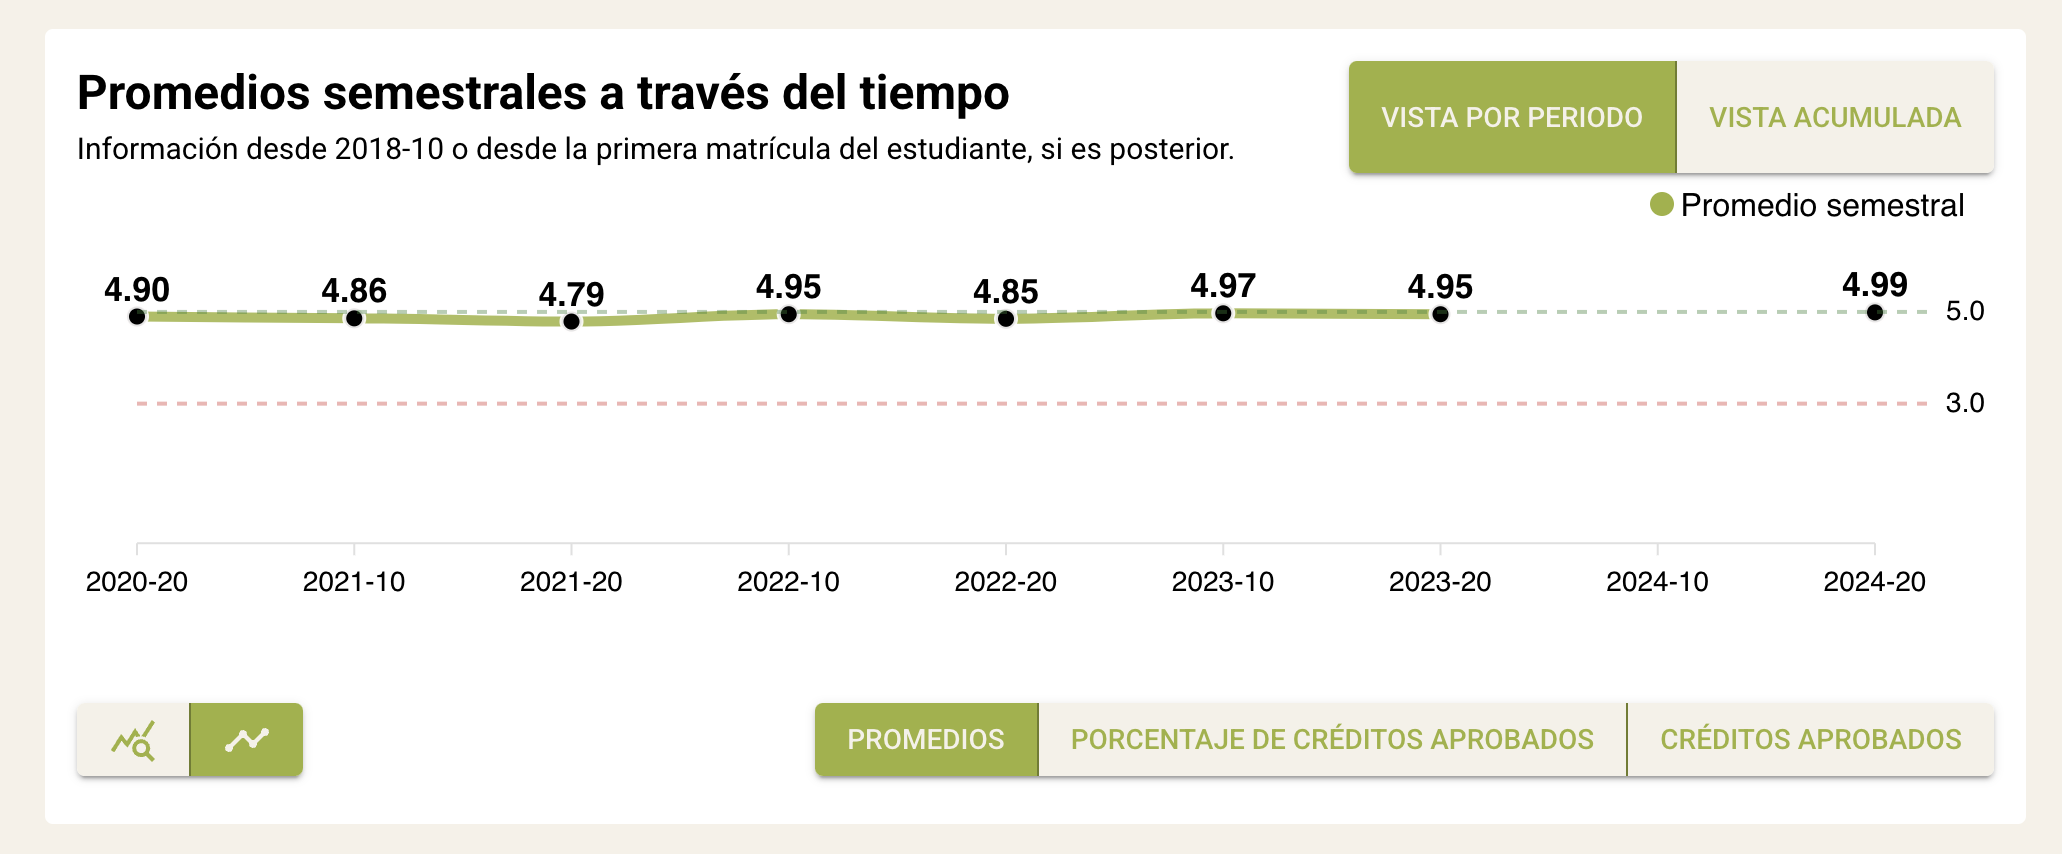
\includegraphics[width=0.8\textwidth]{assets/nes/promedios_estandar.png}
		      \caption{Visualización de promedios semestrales a través del tiempo en escala estándar.}
		      \label{fig:promedios_estandar}
	      \end{figure}

	      En la figura \ref{fig:promedios_estandar} resalta que hay un hueco en la gráfica. Esto puede suceder para alumnos que en un periodo académico determinado no tuvieron un promedio semestral numérico. Lo anterior puede deberse a varias causas; algunas de las más comunes son que el estudiante haya cursado un intercambio académico o una práctica académica, o que únicamente haya visto materias con calificación alfabética (por ejemplo: deportes o cursos de inglés). En estos casos, no se calcula un promedio semestral numérico, lo cual se ve reflejado en la gráfica mediante un salto. Ese espacio no se evidencia en la gráfica de la visualización 1 porque el PGA siempre es numérico, y si en un semestre no hay promedio semestral, el PGA se calcula con los promedios semestrales de los semestres anteriores.

	\item \textbf{Promedios, Vista por periodo, Escala relativa.} Similar a la visualización 2, esta visualización corresponde a la misma información de la visualización 3 pero pone el foco en el comportamiento del promedio semestral del estudiante a lo largo del tiempo. Se presenta en la figura \ref{fig:promedios_relativo}.

	      \begin{figure}[H]
		      \centering
		      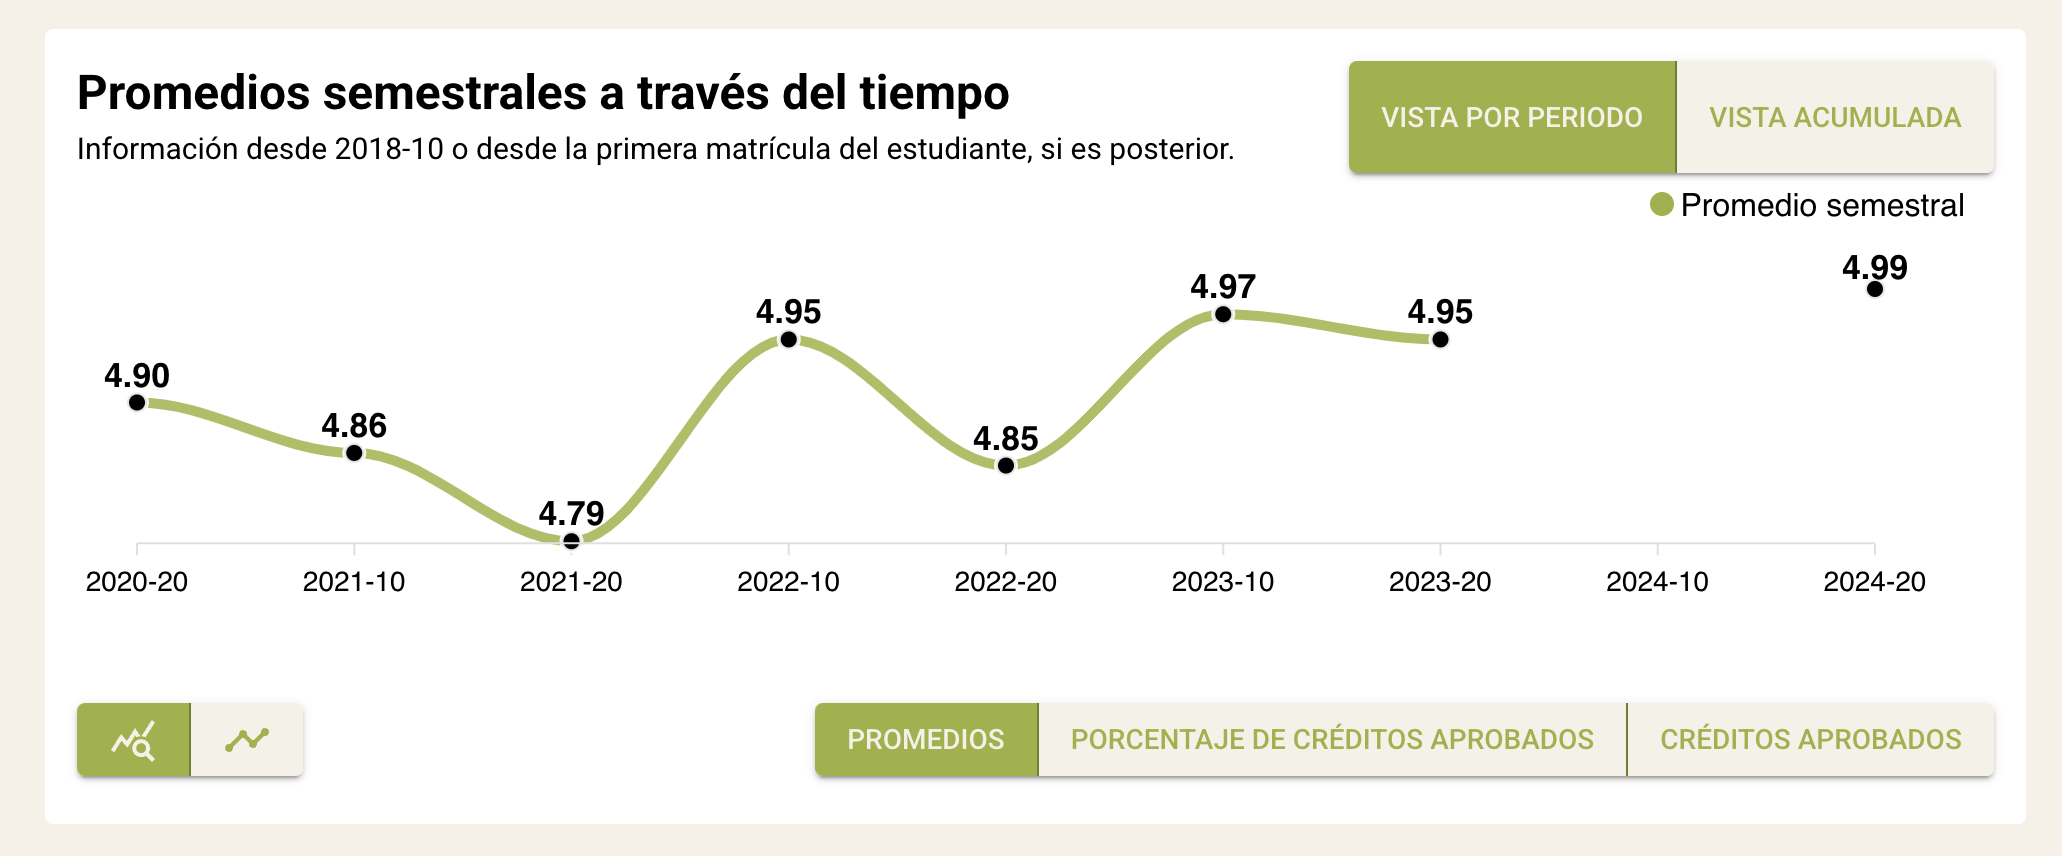
\includegraphics[width=0.8\textwidth]{assets/nes/promedios_relativo.png}
		      \caption{Visualización de promedios semestrales a través del tiempo en escala relativa.}
		      \label{fig:promedios_relativo}
	      \end{figure}

	\item \textbf{Porcentaje de Créditos Aprobados, Vista acumulada, Escala estándar.} Esta visualización se titula \say{Porcentaje acumulado de créditos aprobados} y muestra como ha cambiado el porcentaje de créditos aprobados por el alumno a lo largo del tiempo. En cada periodo, el porcentaje de créditos aprobados es acumulado, por lo cual contempla los periodos anteriores. Se utiliza una escala estándar con un mínimo de 0\% y un máximo de 100\%. Se trazan dos líneas de referencia, que son proporcionales a las trazadas en la visualización 1: la inferior se traza en rojo y corresponde al 60\% de los créditos aprobados; la superior se traza en verde y corresponde al 100\% de los créditos aprobados. Se presenta en la figura \ref{fig:porcentaje_estandar}.

	      \begin{figure}[H]
		      \centering
		      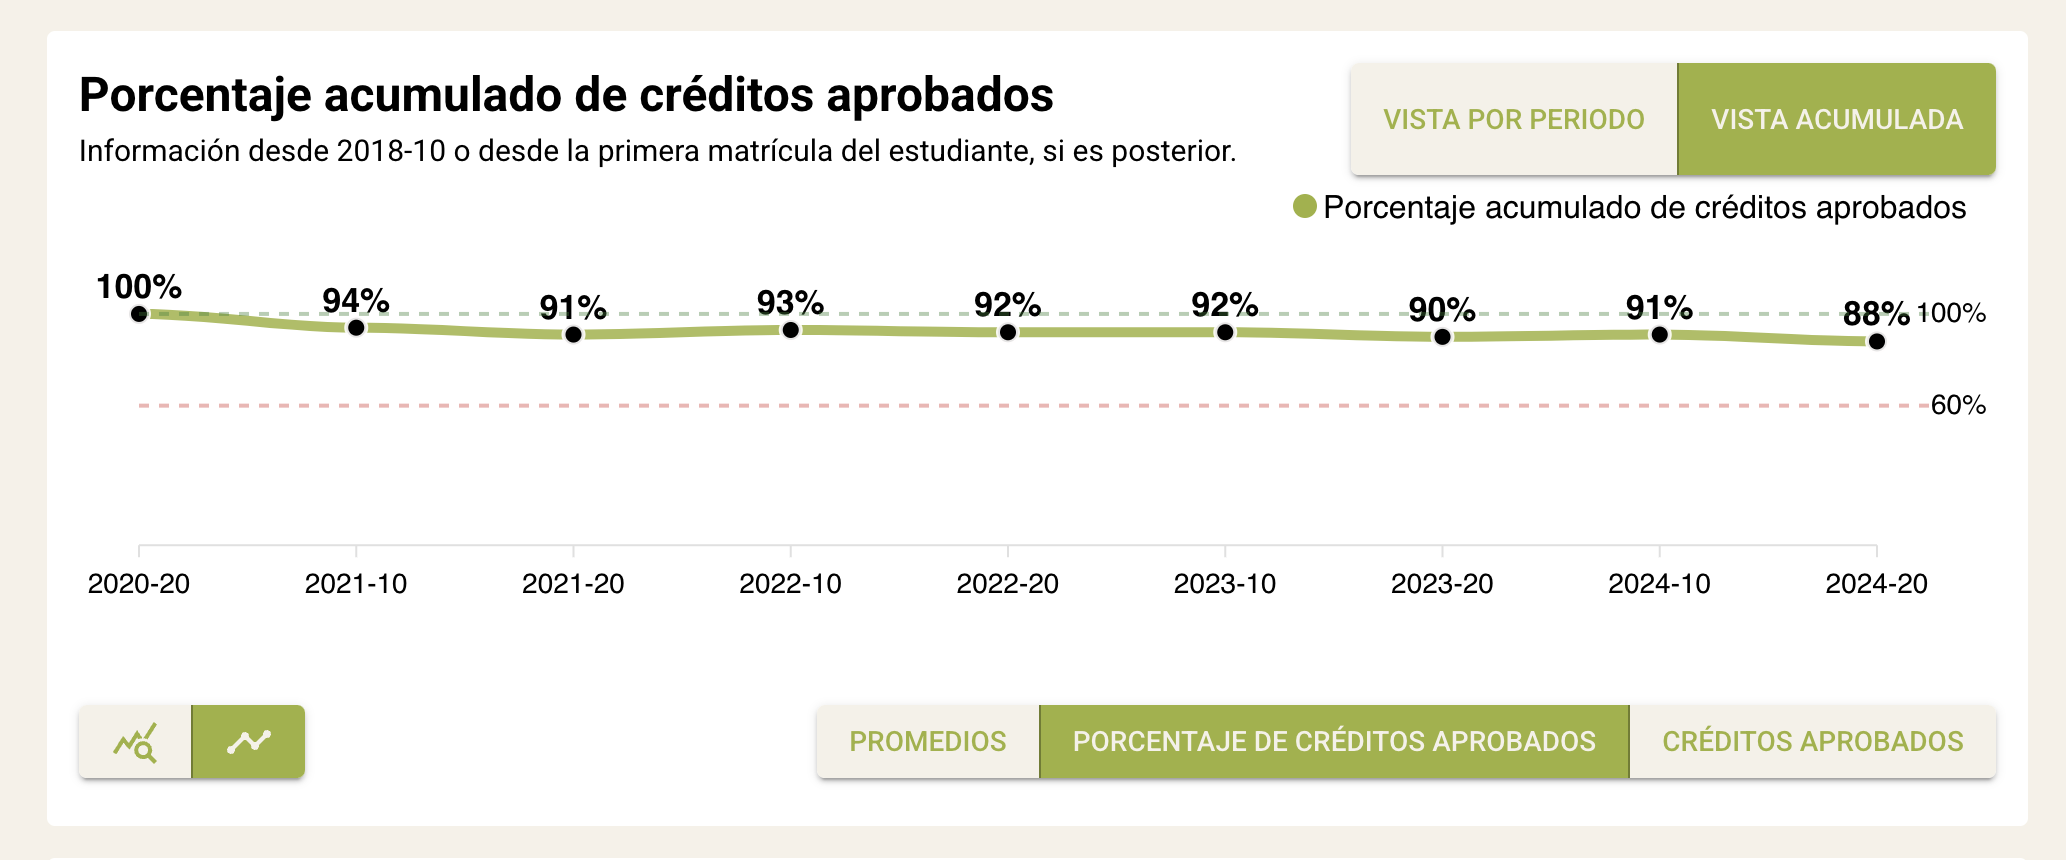
\includegraphics[width=0.8\textwidth]{assets/nes/porcentaje_estandar.png}
		      \caption{Visualización de porcentaje de créditos aprobados a través del tiempo en escala estándar.}
		      \label{fig:porcentaje_estandar}
	      \end{figure}

	\item \textbf{Porcentaje de Créditos Aprobados, Vista acumulada, Escala relativa.} Similar a la visualización 5, esta visualización pone el énfasis en la variabilidad del porcentaje de créditos aprobados del estudiante a lo largo del tiempo, en lugar de en los valores. Se presenta en la figura \ref{fig:porcentaje_relativo}.

	      \begin{figure}[H]
		      \centering
		      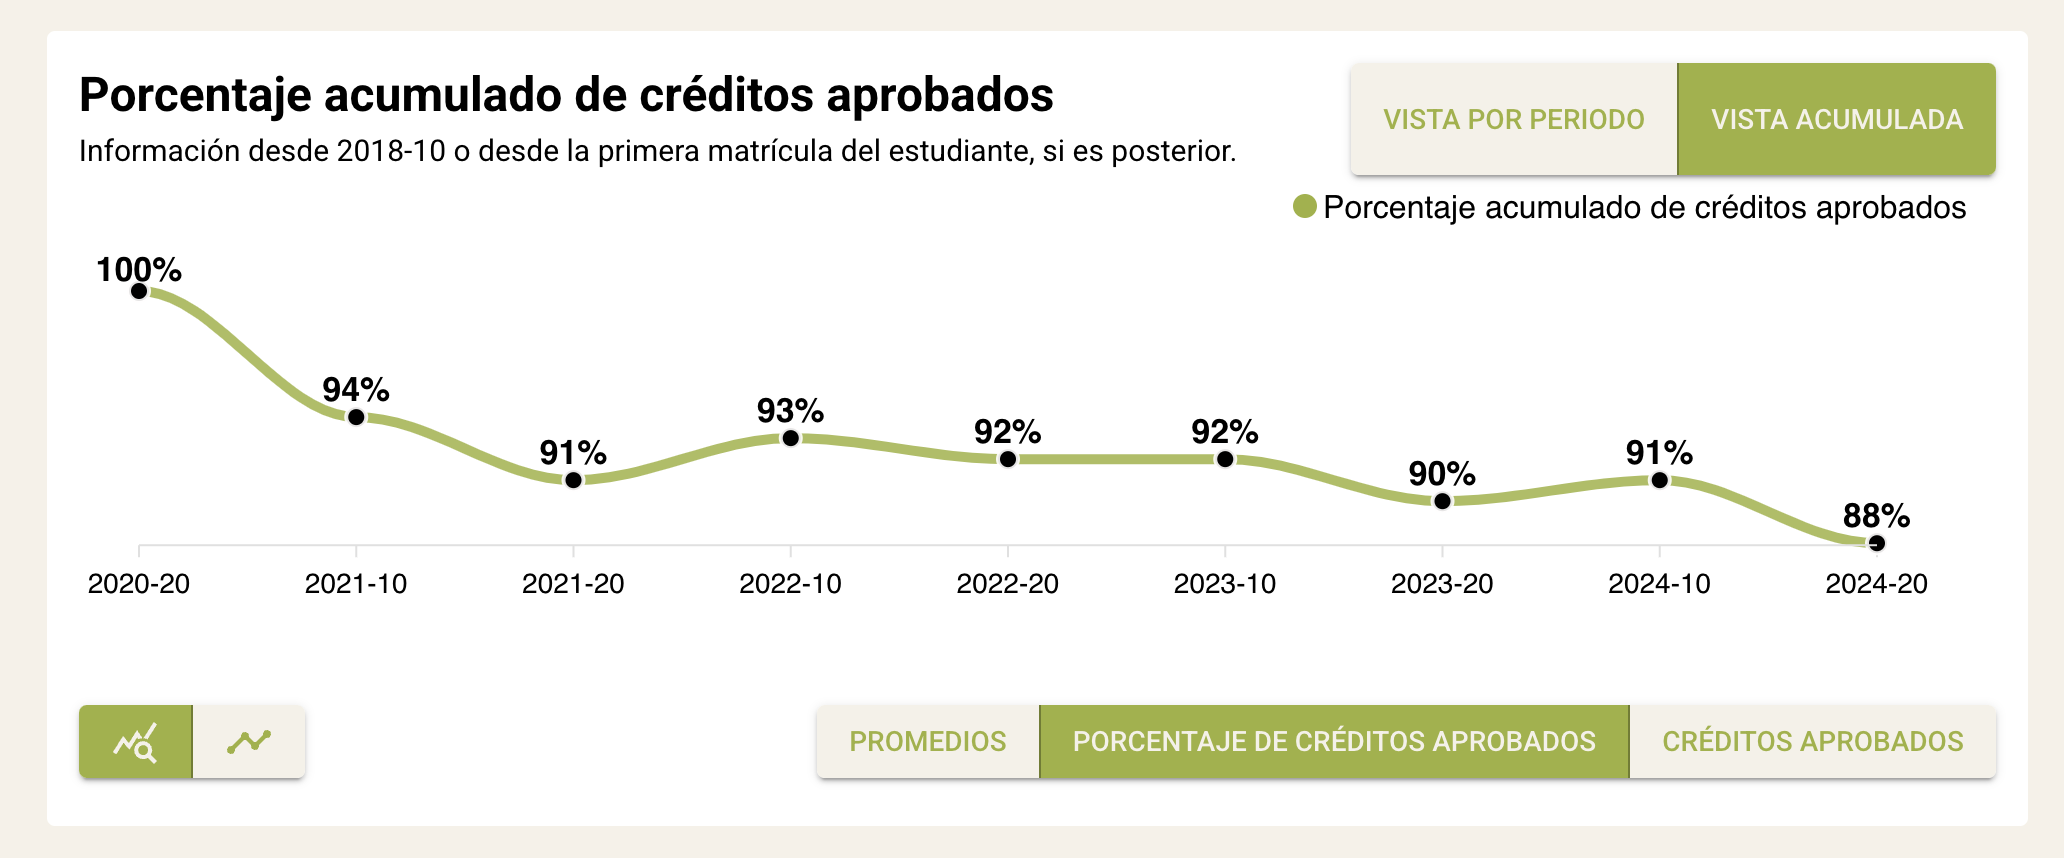
\includegraphics[width=0.8\textwidth]{assets/nes/porcentaje_relativo.png}
		      \caption{Visualización de porcentaje de créditos aprobados a través del tiempo en escala relativa.}
		      \label{fig:porcentaje_relativo}
	      \end{figure}

	\item \textbf{Porcentaje de Créditos Aprobados, Vista por periodo, Escala estándar.} Esta visualización se titula \say{Porcentaje de créditos aprobados por periodo} y muestra el porcentaje de créditos aprobados por el alumno en cada periodo académico, sin contemplar los periodos anteriores. Esto permite estudiar el desempeño del estudiante en cada periodo de forma independiente. Se utiliza la misma escala estándar que en la visualización 5. Se presenta en la figura \ref{fig:porcentaje_periodo_estandar}.

	      \begin{figure}[H]
		      \centering
		      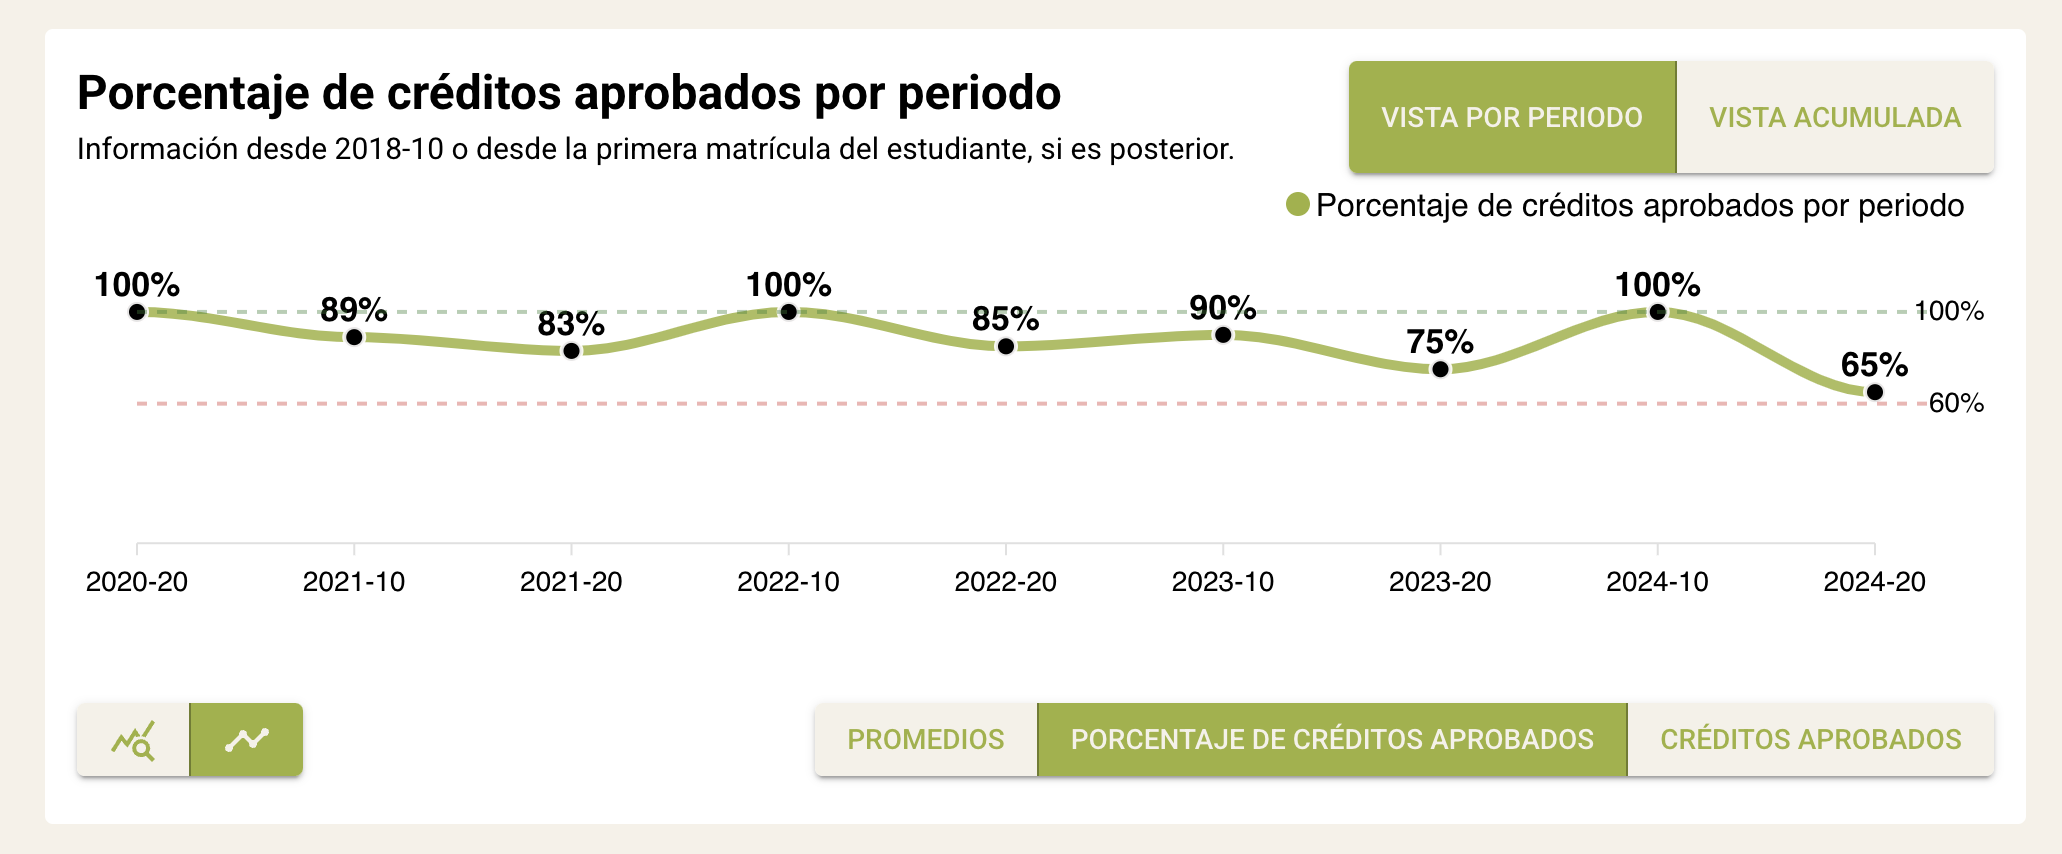
\includegraphics[width=0.8\textwidth]{assets/nes/porcentaje_periodo_estandar.png}
		      \caption{Visualización de porcentaje de créditos aprobados por periodo en escala estándar.}
		      \label{fig:porcentaje_periodo_estandar}
	      \end{figure}

	\item \textbf{Porcentaje de Créditos Aprobados, Vista por periodo, Escala relativa.} Similar a la visualización 7, esta visualización pone el énfasis en el comportamiento del porcentaje de créditos aprobados del estudiante en cada periodo académico. Se presenta en la figura \ref{fig:porcentaje_periodo_relativo}.

	      \begin{figure}[H]
		      \centering
		      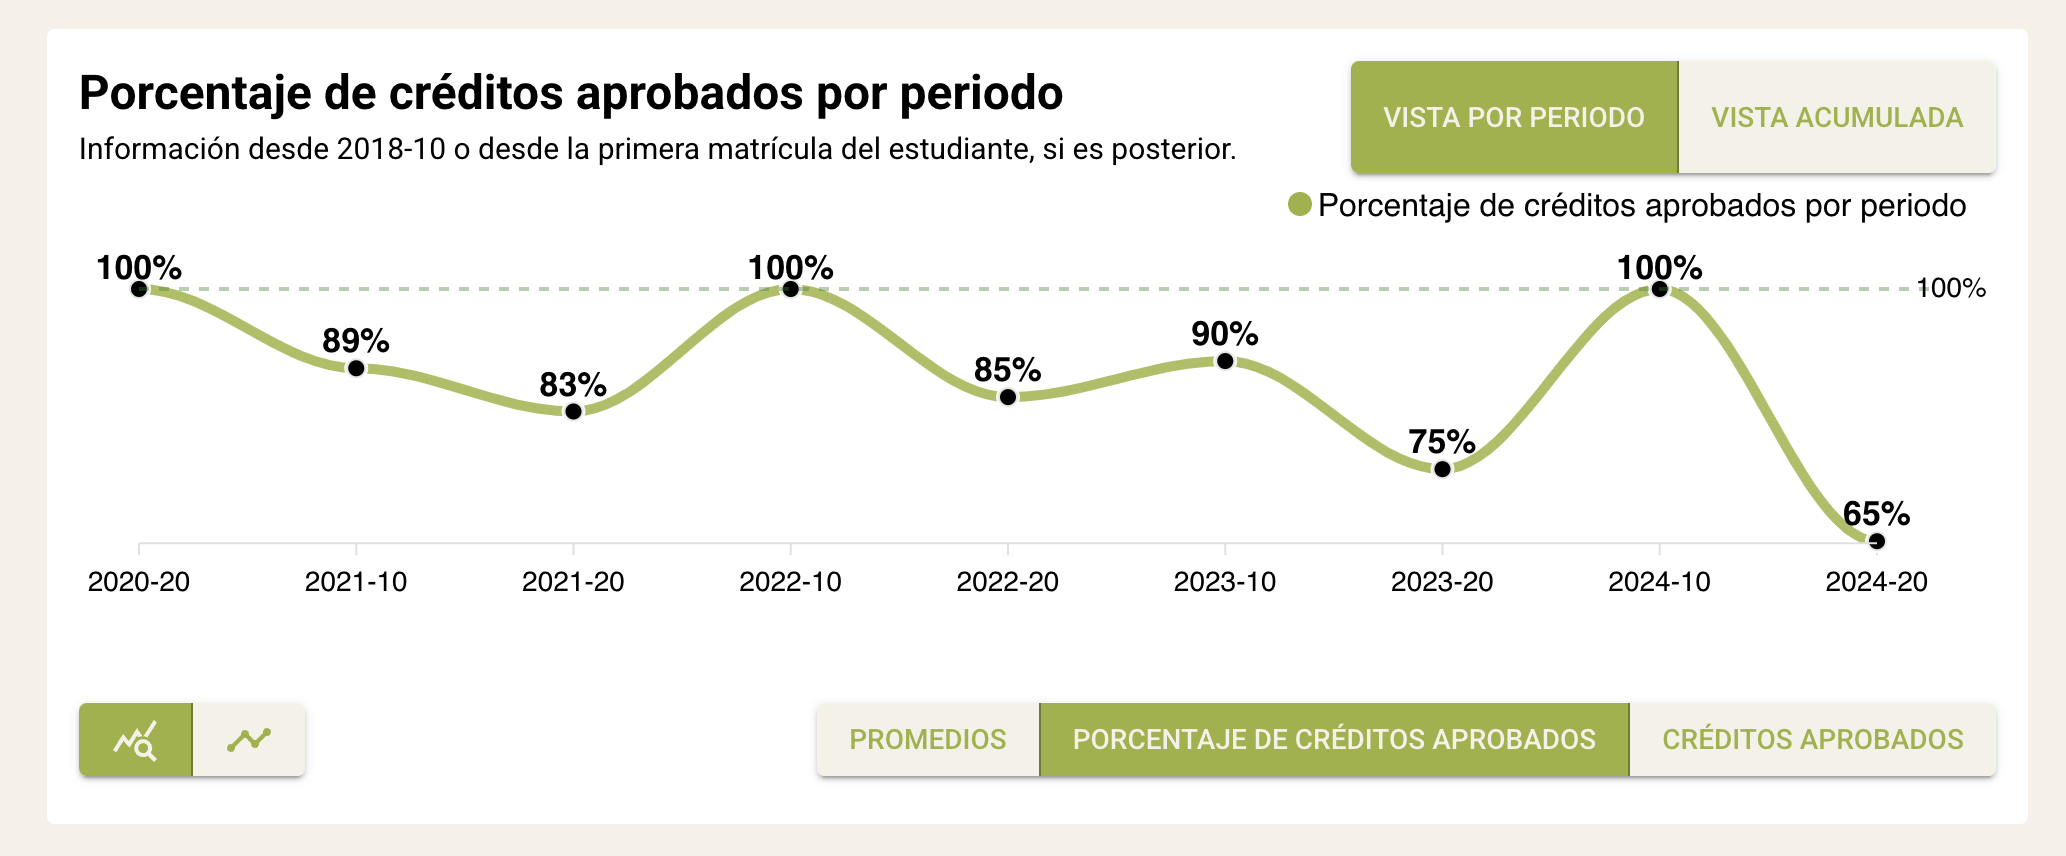
\includegraphics[width=0.8\textwidth]{assets/nes/porcentaje_periodo_relativo.png}
		      \caption{Visualización de porcentaje de créditos aprobados por periodo en escala relativa.}
		      \label{fig:porcentaje_periodo_relativo}
	      \end{figure}

	\item \textbf{Créditos Aprobados, Vista acumulada, Escala estándar.} Esta visualización se titula \say{Créditos aprobados acumulados} y muestra la cantidad de créditos aprobados por el estudiante a lo largo del tiempo. En cada periodo, los créditos aprobados son acumulados, por lo cual contempla los periodos anteriores. La escala estándar usa un mínimo de 0 créditos y utiliza como máximo el número de créditos aprobados por el alumno hasta la fecha. No se trazan líneas de referencia, pues no tiene sentido para esta gráfica, en la que un valor bajo en el total de créditos aprobados no indica un mal rendimiento sino simplemente una etapa temprana en la carrera del estudiante. Se presenta en la figura \ref{fig:creditos_estandar}.

	      \begin{figure}[H]
		      \centering
		      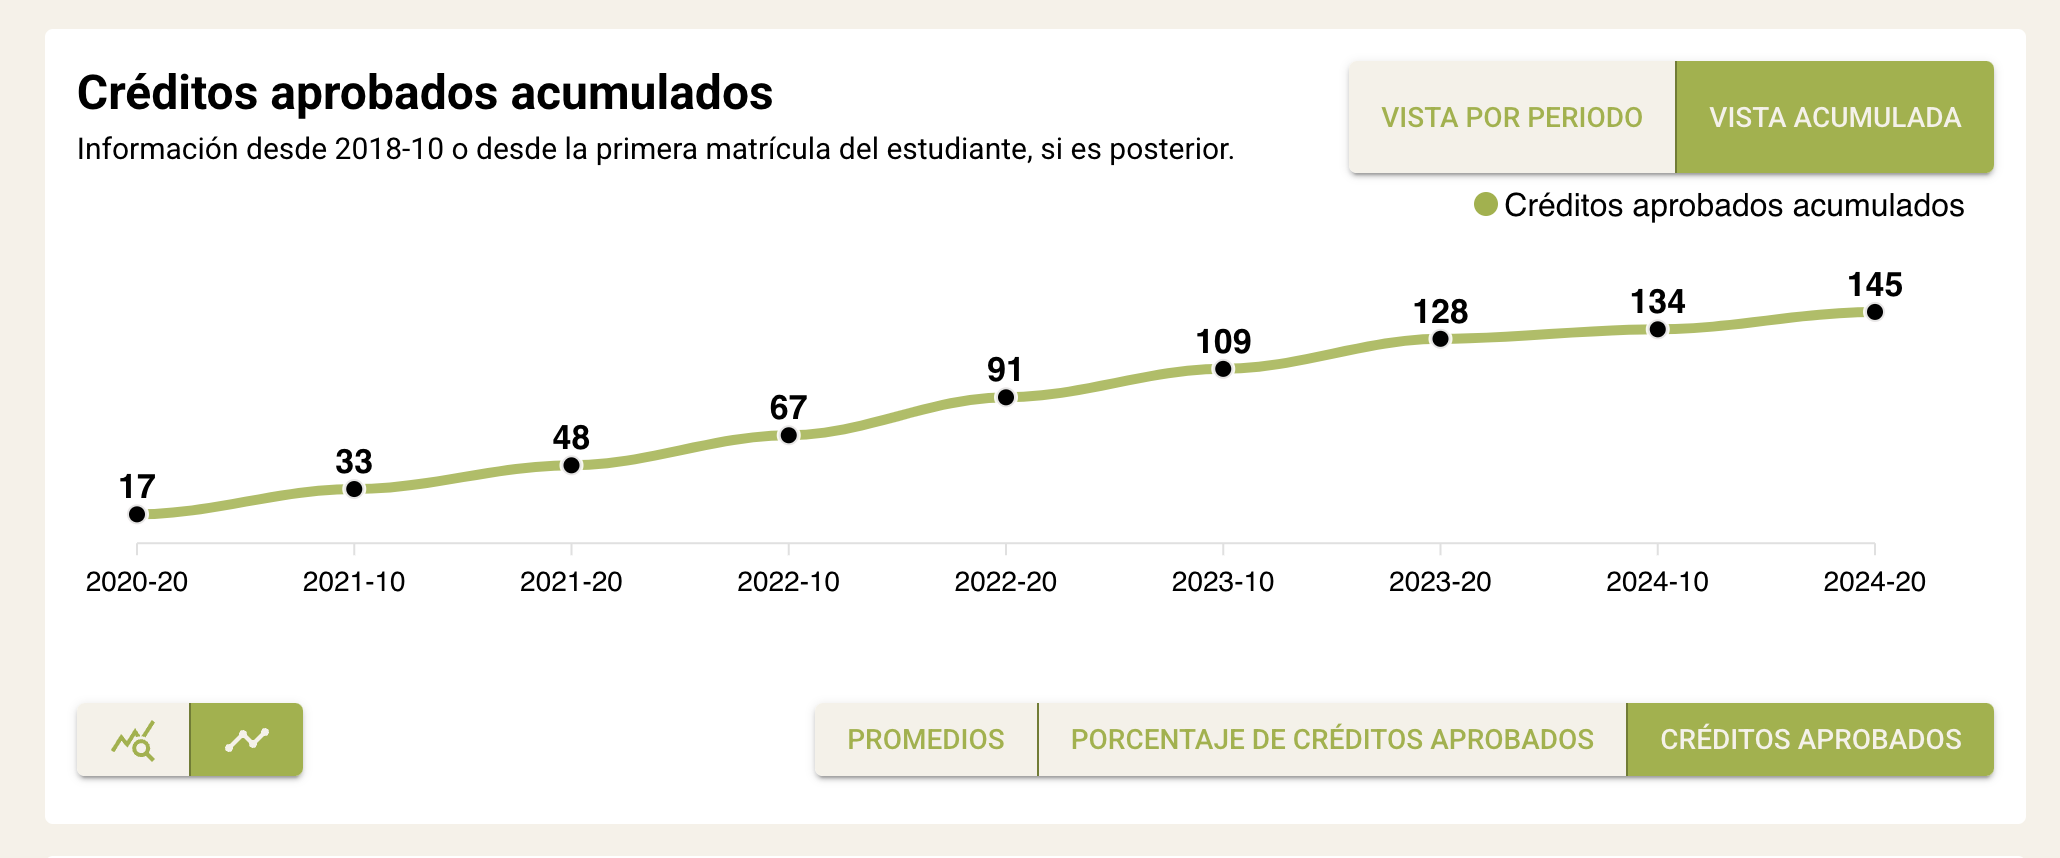
\includegraphics[width=0.8\textwidth]{assets/nes/creditos_estandar.png}
		      \caption{Visualización de créditos aprobados a través del tiempo en escala estándar.}
		      \label{fig:creditos_estandar}
	      \end{figure}

	\item \textbf{Créditos Aprobados, Vista acumulada, Escala relativa.} Esta visualización resulta muy similar a la anterior, con la única diferencia en que el valor mínimo es el número de créditos aprobados por el alumno en el periodo más temprano, en lugar de ser 0 créditos. Se presenta en la figura \ref{fig:creditos_relativo}.

	      \begin{figure}[H]
		      \centering
		      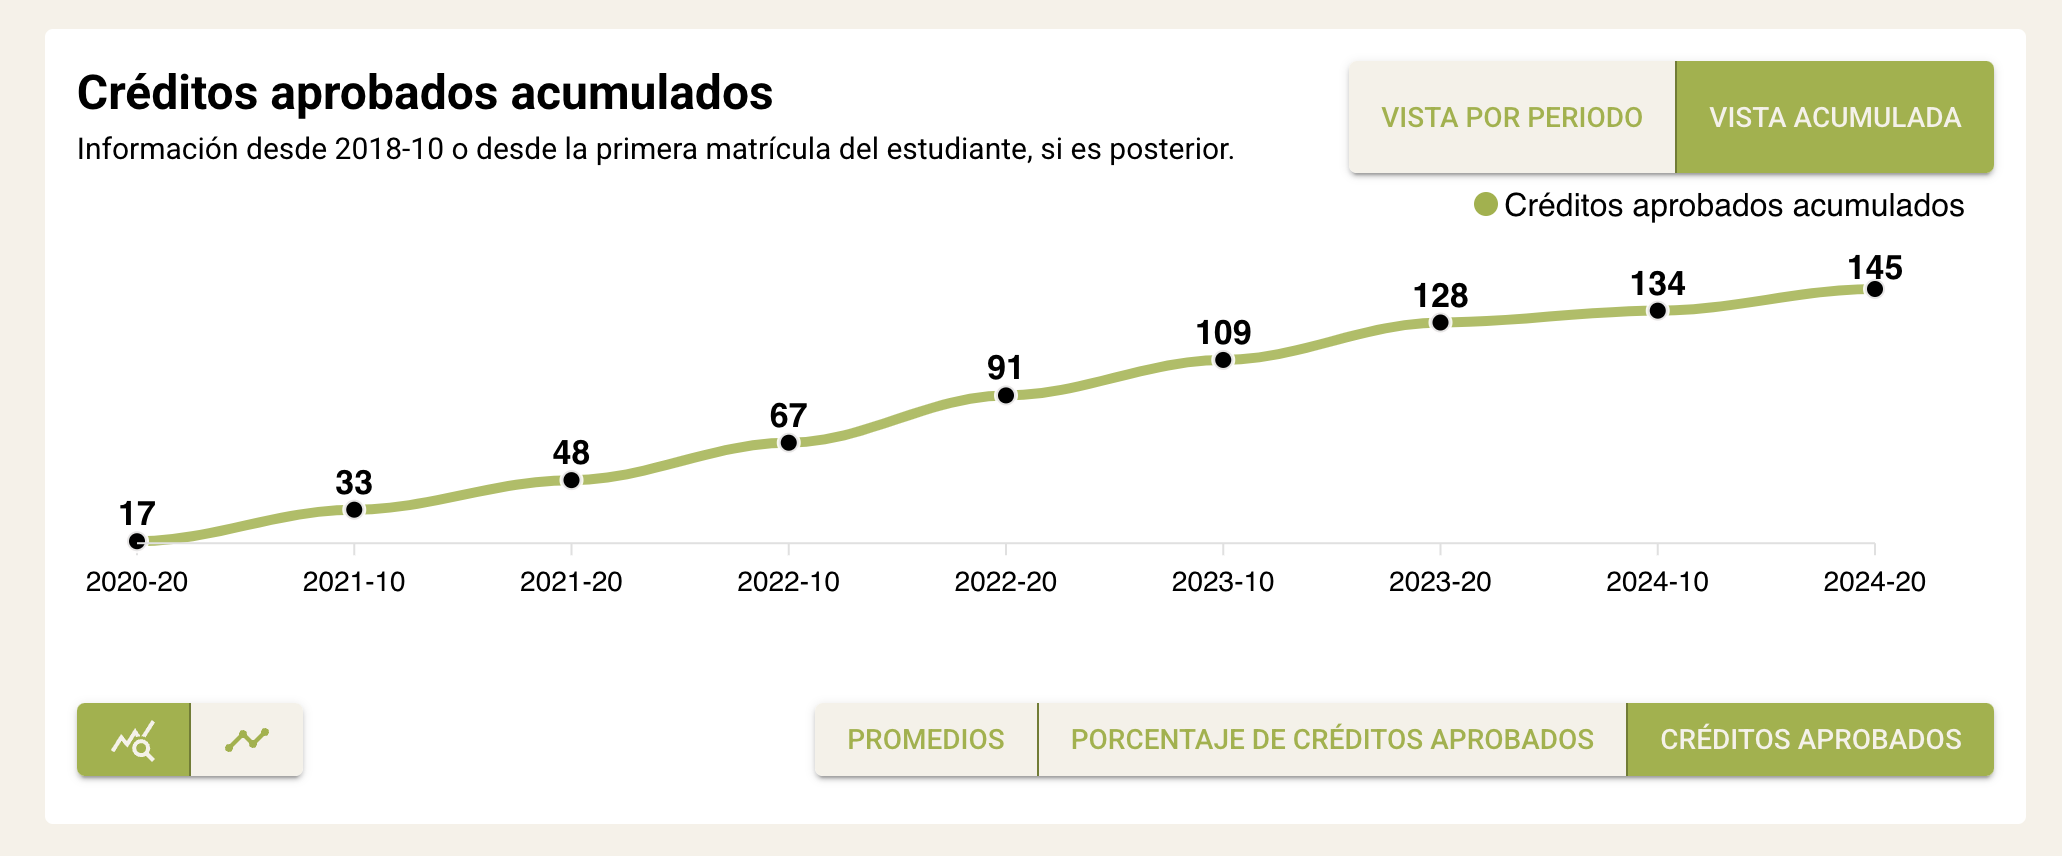
\includegraphics[width=0.8\textwidth]{assets/nes/creditos_relativo.png}
		      \caption{Visualización de créditos aprobados a través del tiempo en escala relativa.}
		      \label{fig:creditos_relativo}
	      \end{figure}

	\item \textbf{Créditos Aprobados, Vista por periodo, Escala estándar.} Esta visualización se titula \say{Créditos aprobados por periodo} y muestra la cantidad de créditos aprobados por el estudiante en cada periodo académico, sin contemplar los periodos anteriores. La escala estándar usa un mínimo de 0 créditos y un máximo que depende del número de créditos aprobados en el periodo con más créditos aprobados. Se traza una línea de referencia, a la altura de los 11 créditos, que no necesariamente tiene connotaciones negativas, teniendo en cuenta que el alumno puede haber cursado matrículas parciales. Se presenta en la figura \ref{fig:creditos_periodo_estandar}.

	      \begin{figure}[H]
		      \centering
		      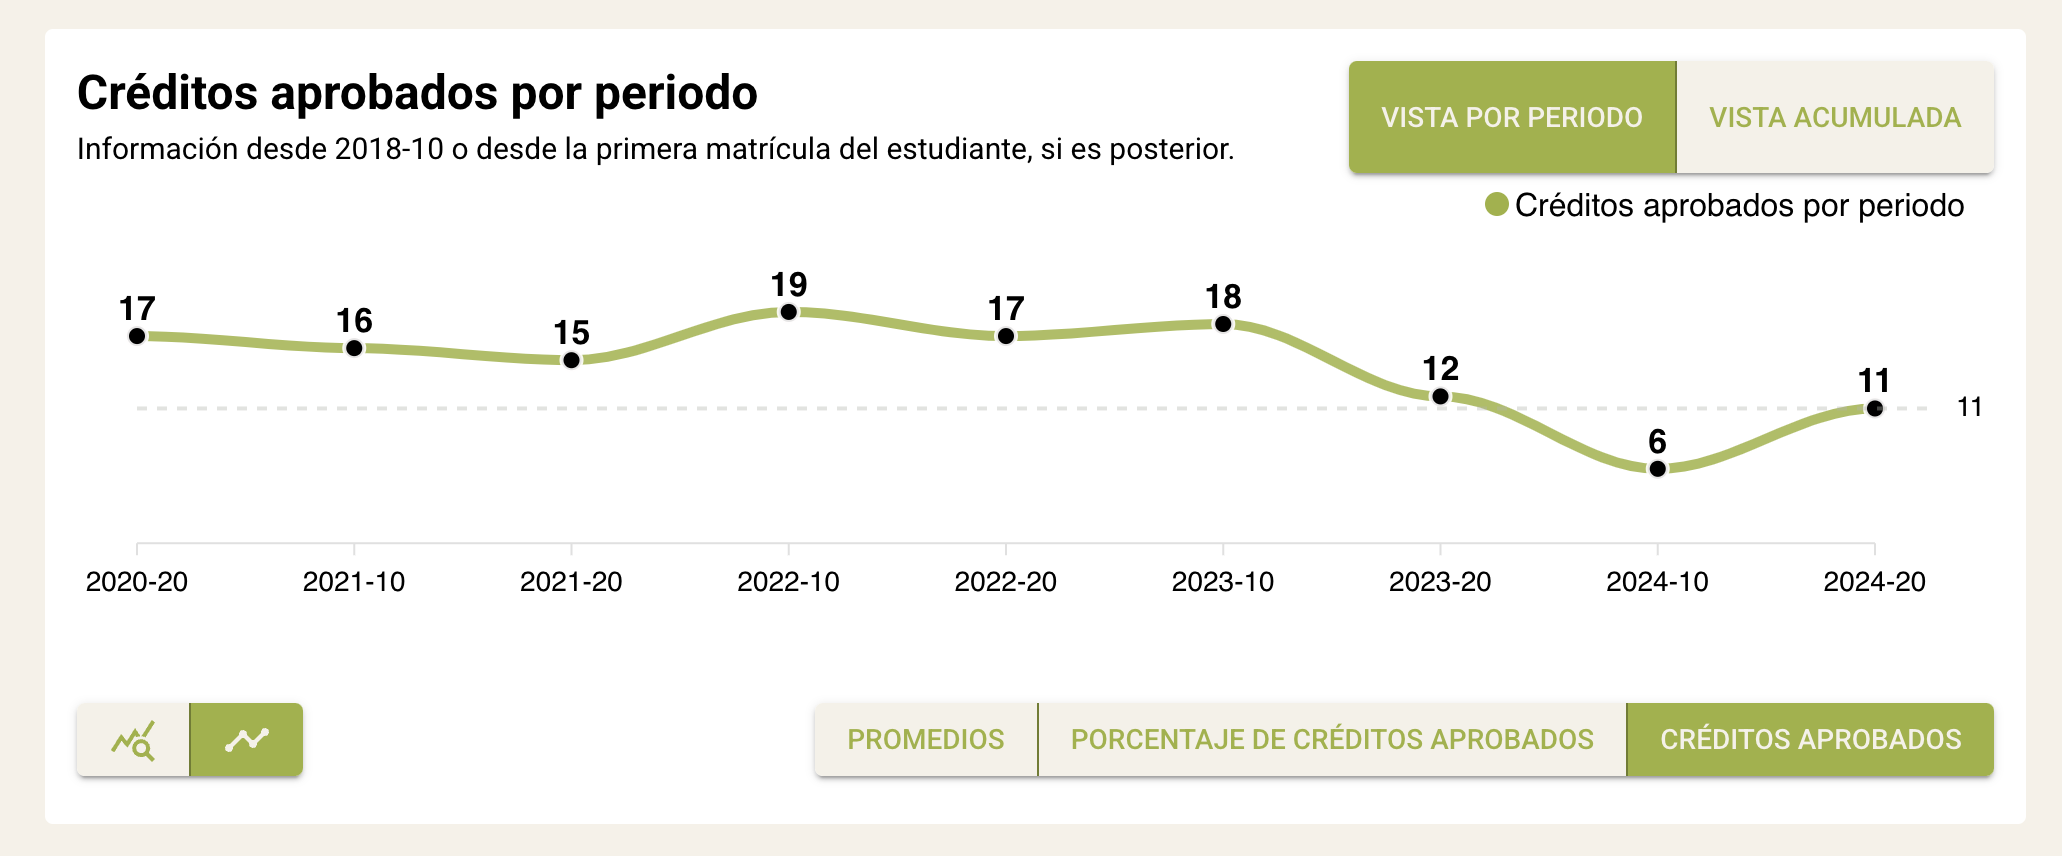
\includegraphics[width=0.8\textwidth]{assets/nes/creditos_periodo_estandar.png}
		      \caption{Visualización de créditos aprobados por periodo en escala estándar.}
		      \label{fig:creditos_periodo_estandar}
	      \end{figure}

	\item \textbf{Créditos Aprobados, Vista por periodo, Escala relativa.} Esta última visualización presenta la misma información que la visualización 11, pero pone el énfasis en el comportamiento del número de créditos aprobados por el estudiante en cada periodo académico. Se presenta en la figura \ref{fig:creditos_periodo_relativo}.

	      \begin{figure}[H]
		      \centering
		      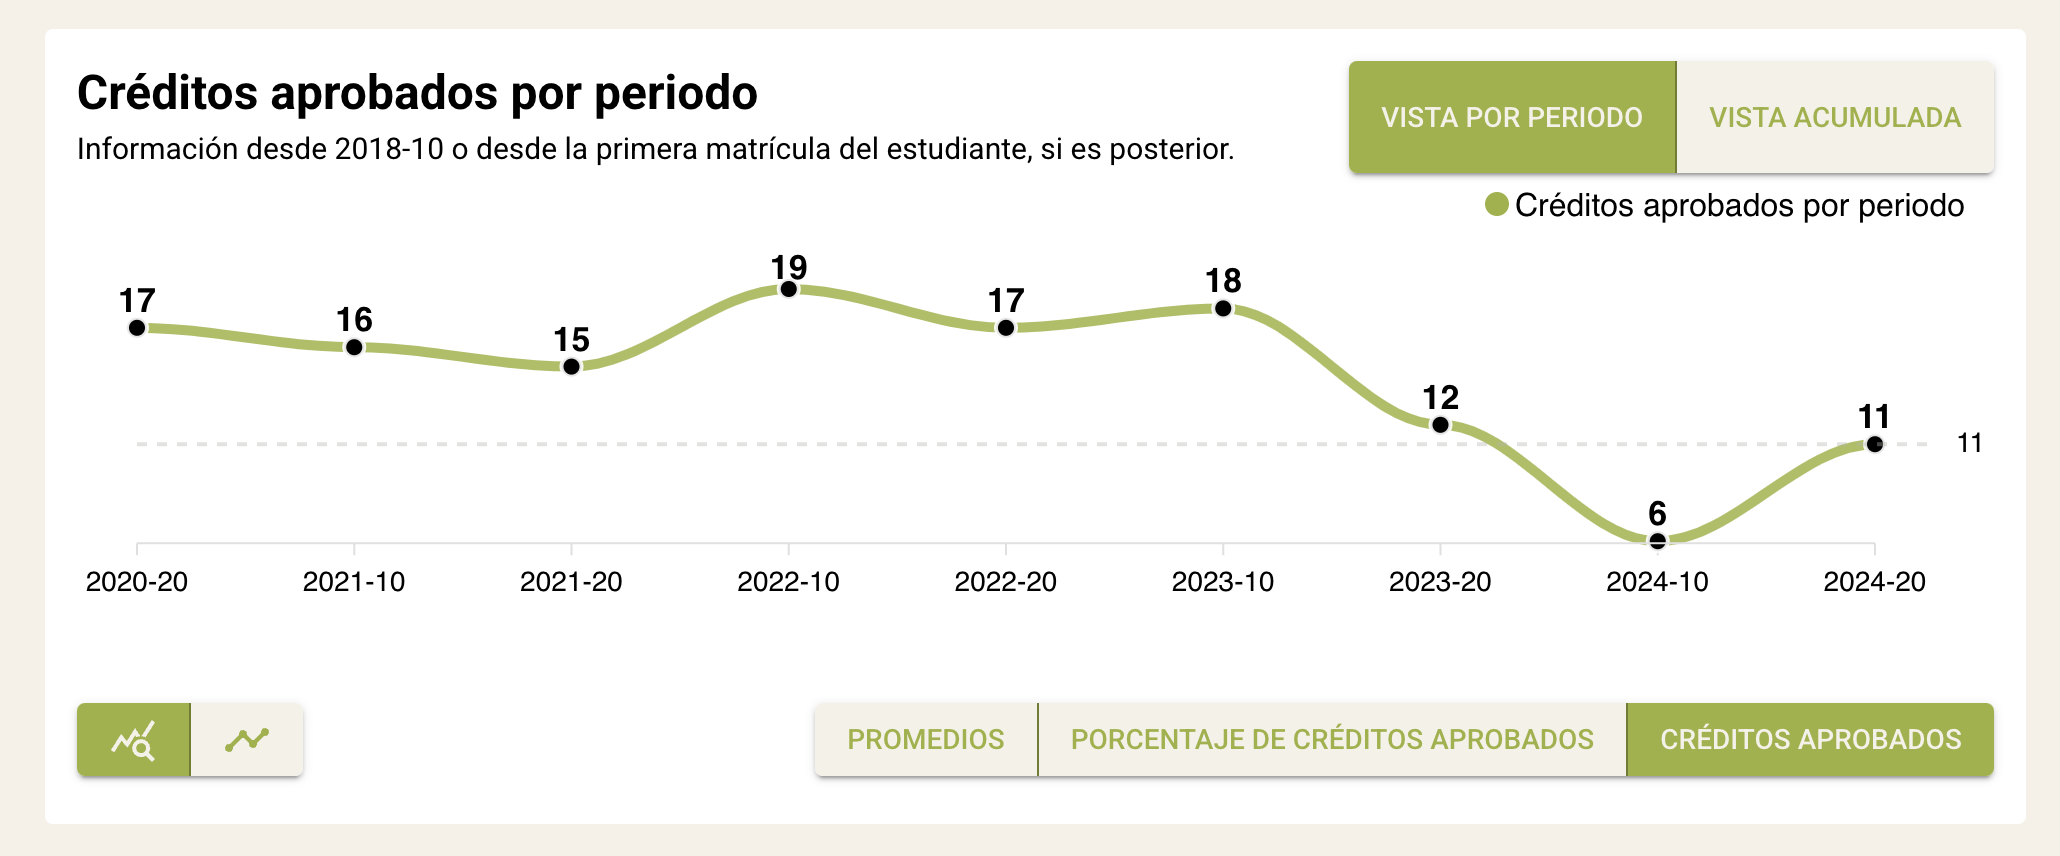
\includegraphics[width=0.8\textwidth]{assets/nes/creditos_periodo_relativo.png}
		      \caption{Visualización de créditos aprobados por periodo en escala relativa.}
		      \label{fig:creditos_periodo_relativo}
	      \end{figure}
\end{enumerate}

\paragraph{Tabla de créditos inscritos} La tabla de créditos inscritos es el siguiente componente de la pestaña de Desempeño. Se muestra en la figura \ref{fig:tabla_creditos}. La primera fila de la tabla proporciona un resumen del total de créditos inscritos por el alumno, clasificándolos en \textit{aprobados}, \textit{reprobados}, \textit{retirados}, \textit{incompletos} y \textit{pendientes}. La segunda fila de la tabla permite al usuario visualizar ese desglose de los créditos inscritos pero con relación a un área de conocimiento específica, que el usuario selecciona de un menú desplegable. Por ejemplo, para los estudiantes de ingeniería, se puede seleccionar las áreas de matemáticas, física o su ingeniería específica. La tabla se actualiza automáticamente al seleccionar un área de conocimiento distinta. Como interacción adicional, la tabla incluye la posibilidad de alternar los valores desplegados como  cantidad absoluta de créditos o como porcentaje del total de créditos inscritos, facilitando el análisis de los datos por parte del usuario.

\begin{figure}[H]
	\centering
	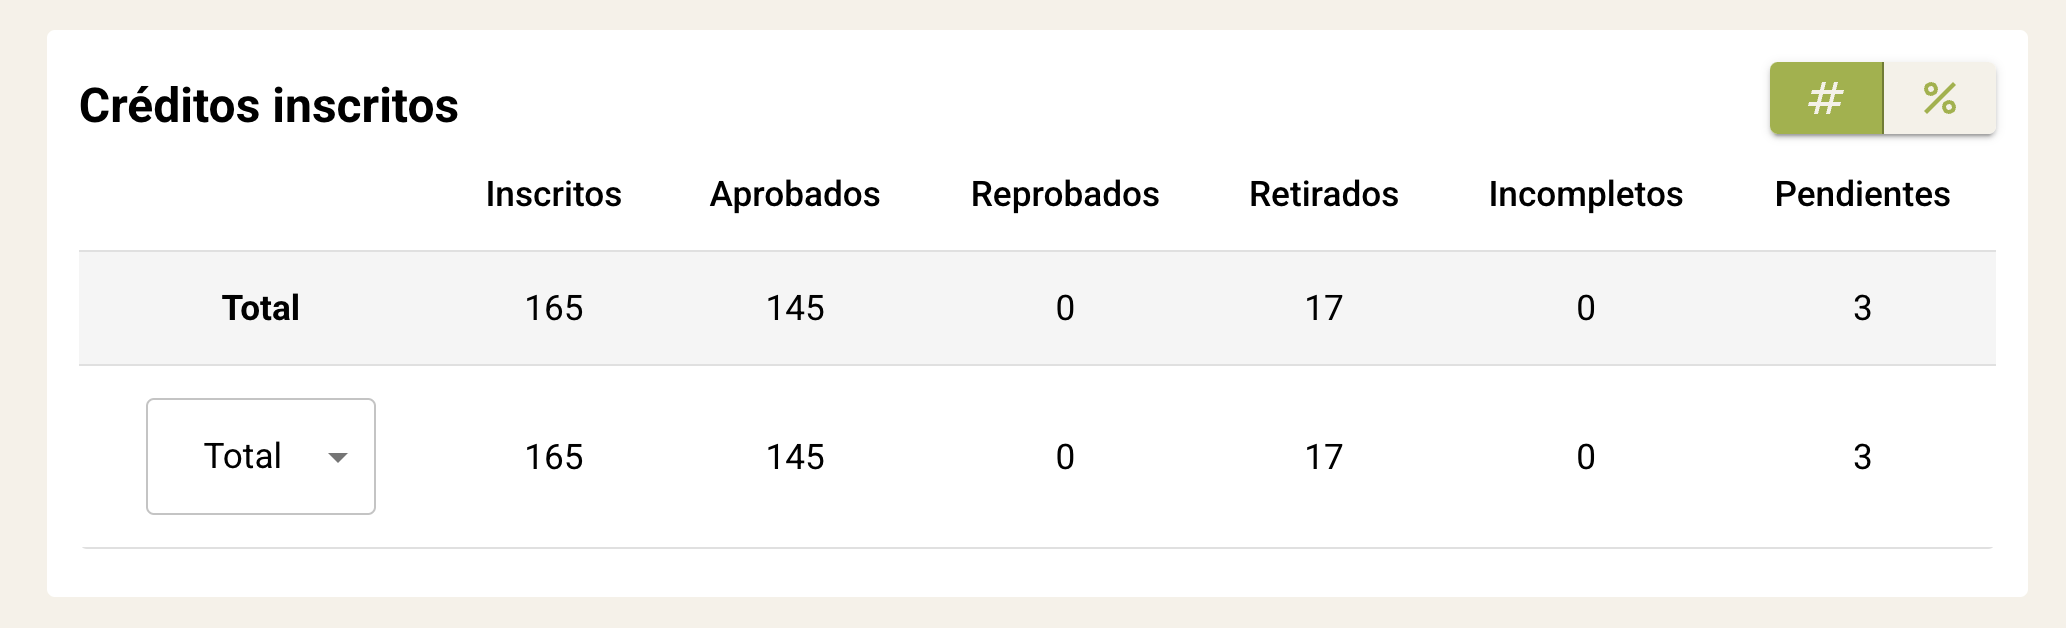
\includegraphics[width=0.8\textwidth]{assets/nes/tabla_creditos.png}
	\caption{Tabla de créditos inscritos.}
	\label{fig:tabla_creditos}
\end{figure}

\paragraph{Gráfica de créditos por periodo} Tras lo anterior, aparece la gráfica de créditos por periodo, exhibida en la figura \ref{fig:grafica_creditos}. Esta gráfica desglosa el número de créditos aprobados, retirados y reprobados en cada periodo académico. Traza una curva para cada uno, pintando los créditos aprobados en verde, los retirados en azul y los reprobados en rojo. Esta gráfica, al igual que la primera, también cuenta con múltiples representaciones. Sin embargo, en ese caso es más sensato explicar las posibles interacciones de la gráfica, sin necesidad de listar las doce visualizaciones posibles.

\begin{figure}[H]
	\centering
	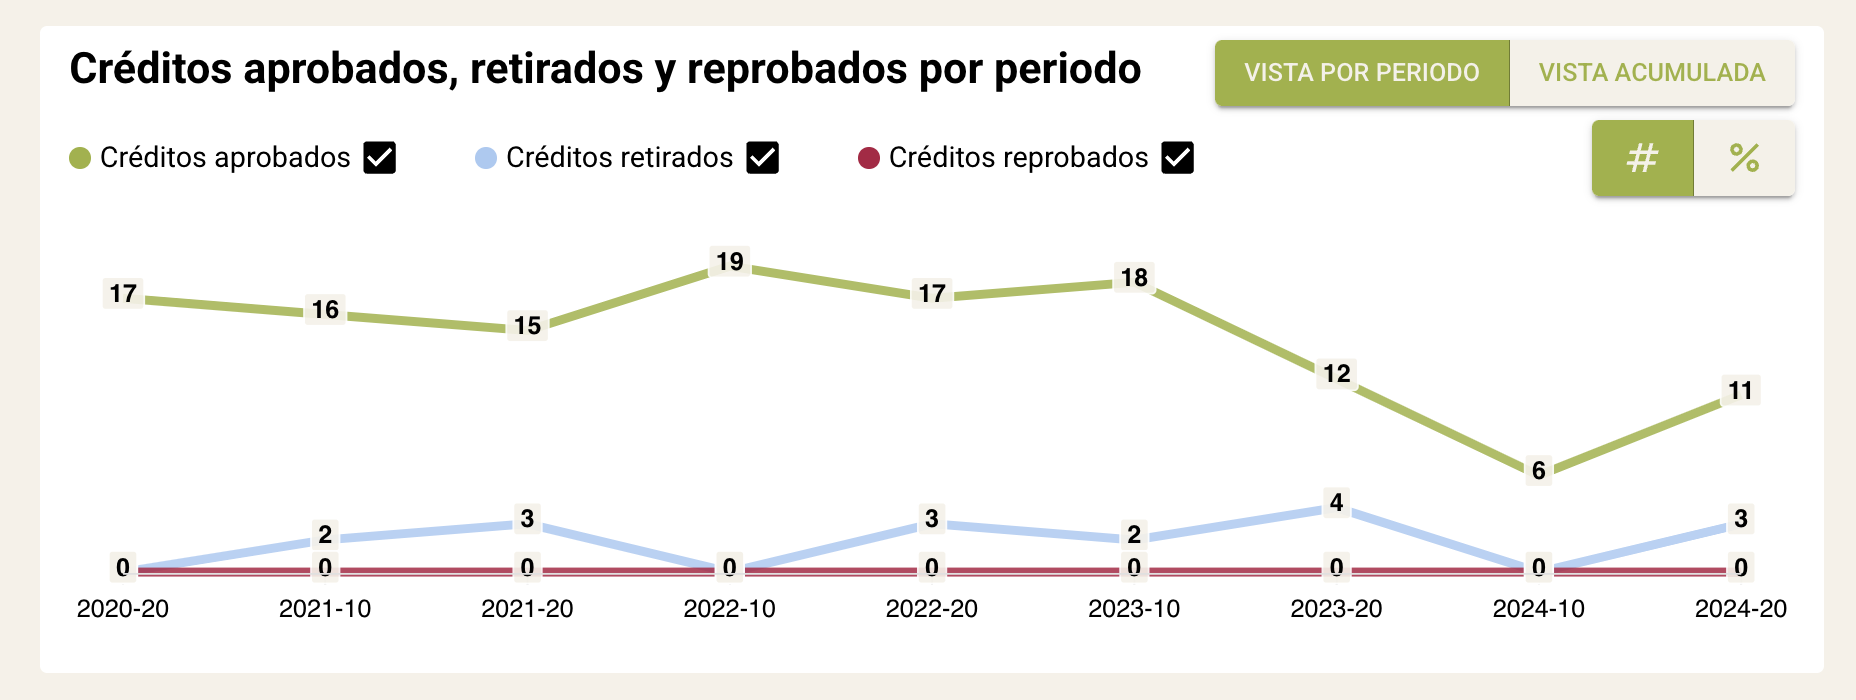
\includegraphics[width=0.8\textwidth]{assets/nes/grafica_creditos.png}
	\caption{Gráfica de créditos por periodo.}
	\label{fig:grafica_creditos}
\end{figure}

\begin{itemize}
	\item \textbf{Esconder alguna, dos o todas las curvas.} La gráfica permite al usuario seleccionar cuáles curvas desea visualizar. Por defecto, se muestran todas las curvas, pero el usuario puede deseleccionar alguna o todas las curvas para enfocarse en una sola o en contrastar dos curvas. Esto resulta útil para reducir el ruido en análisis específicos, como comparar el número de créditos aprobados con el número de créditos reprobados, determinar el comportamiento de específicamente los créditos retirados, entre otros. En la figura \ref{fig:creditos_retirados} se muestra un ejemplo en el que se han deseleccionado las curvas de créditos aprobados y reprobados, dejando solo la curva de créditos retirados.

	      \begin{figure}[H]
		      \centering
		      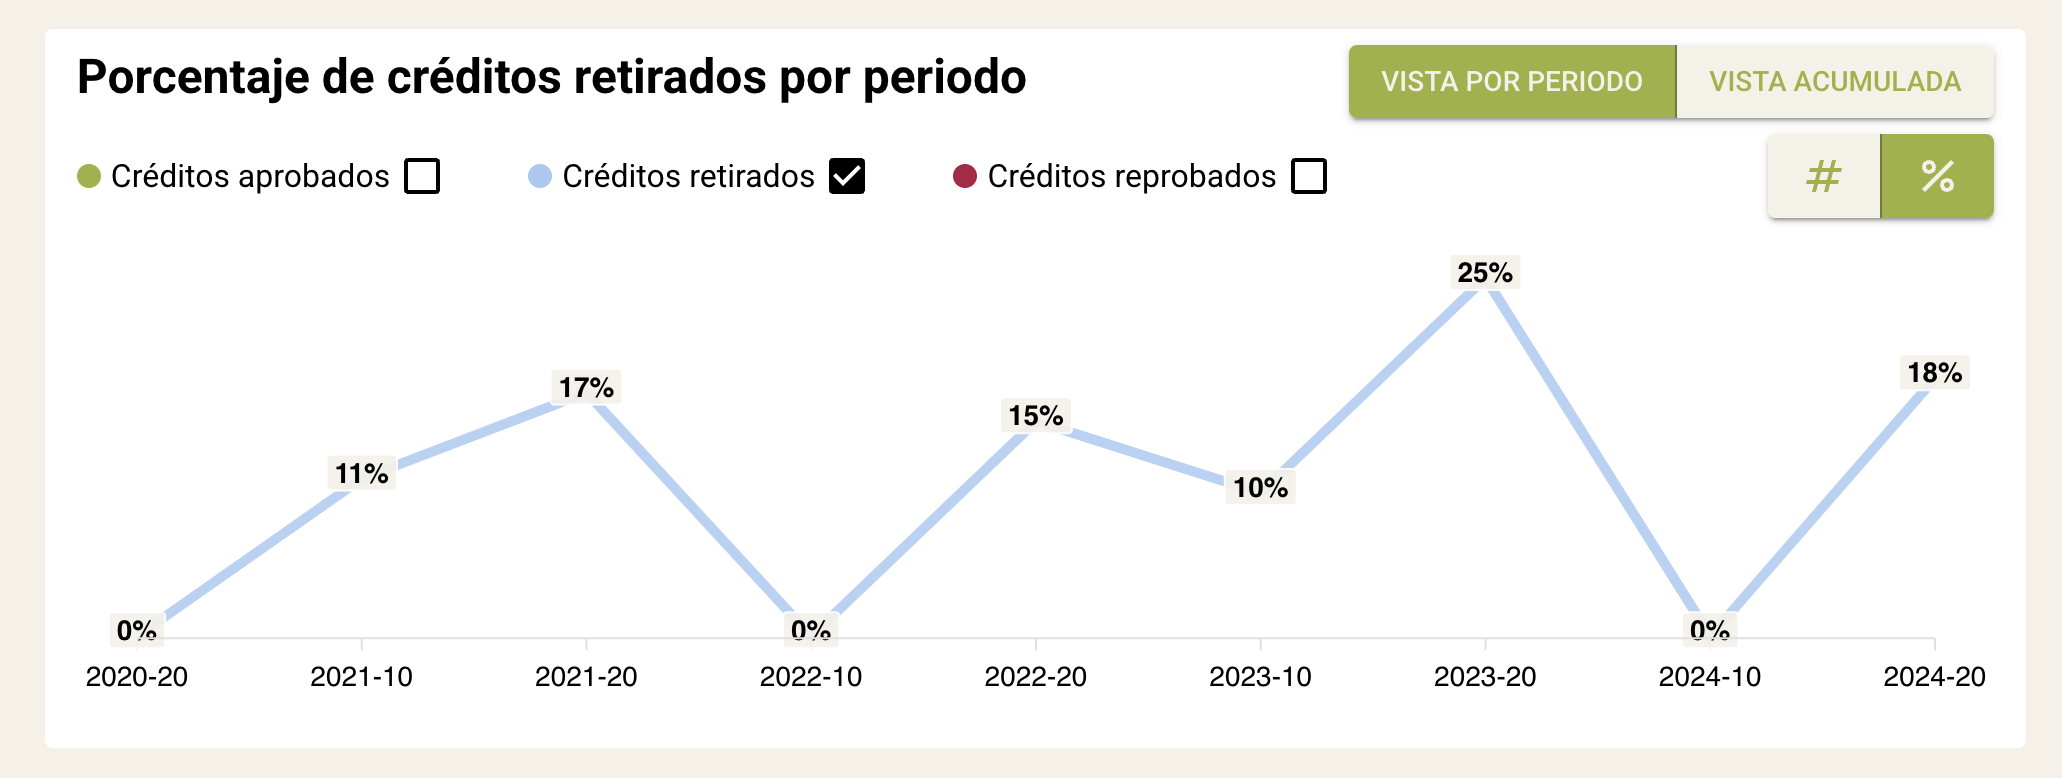
\includegraphics[width=0.8\textwidth]{assets/nes/creditos_retirados.png}
		      \caption{Gráfica de créditos por periodo con solo la curva de créditos retirados.}
		      \label{fig:creditos_retirados}
	      \end{figure}

	\item \textbf{Vista por periodo o acumulada.} Al igual que la gráfica central, esta de créditos por periodo permite al usuario alternar entre una vista por periodo y una vista acumulada. La vista por periodo muestra el comportamiento de los créditos aprobados, retirados y reprobados en cada periodo académico, mientras que la vista acumulada muestra la evolución de esos créditos a lo largo del tiempo. La vista acumulada es particularmente útil para ver cómo el número de créditos aprobados, retirados y reprobados ha cambiado a lo largo de la carrera del estudiante. La figura \ref{fig:creditos_acumulados} muestra un ejemplo de la gráfica de créditos por periodo en vista acumulada.

	      \begin{figure}[H]
		      \centering
		      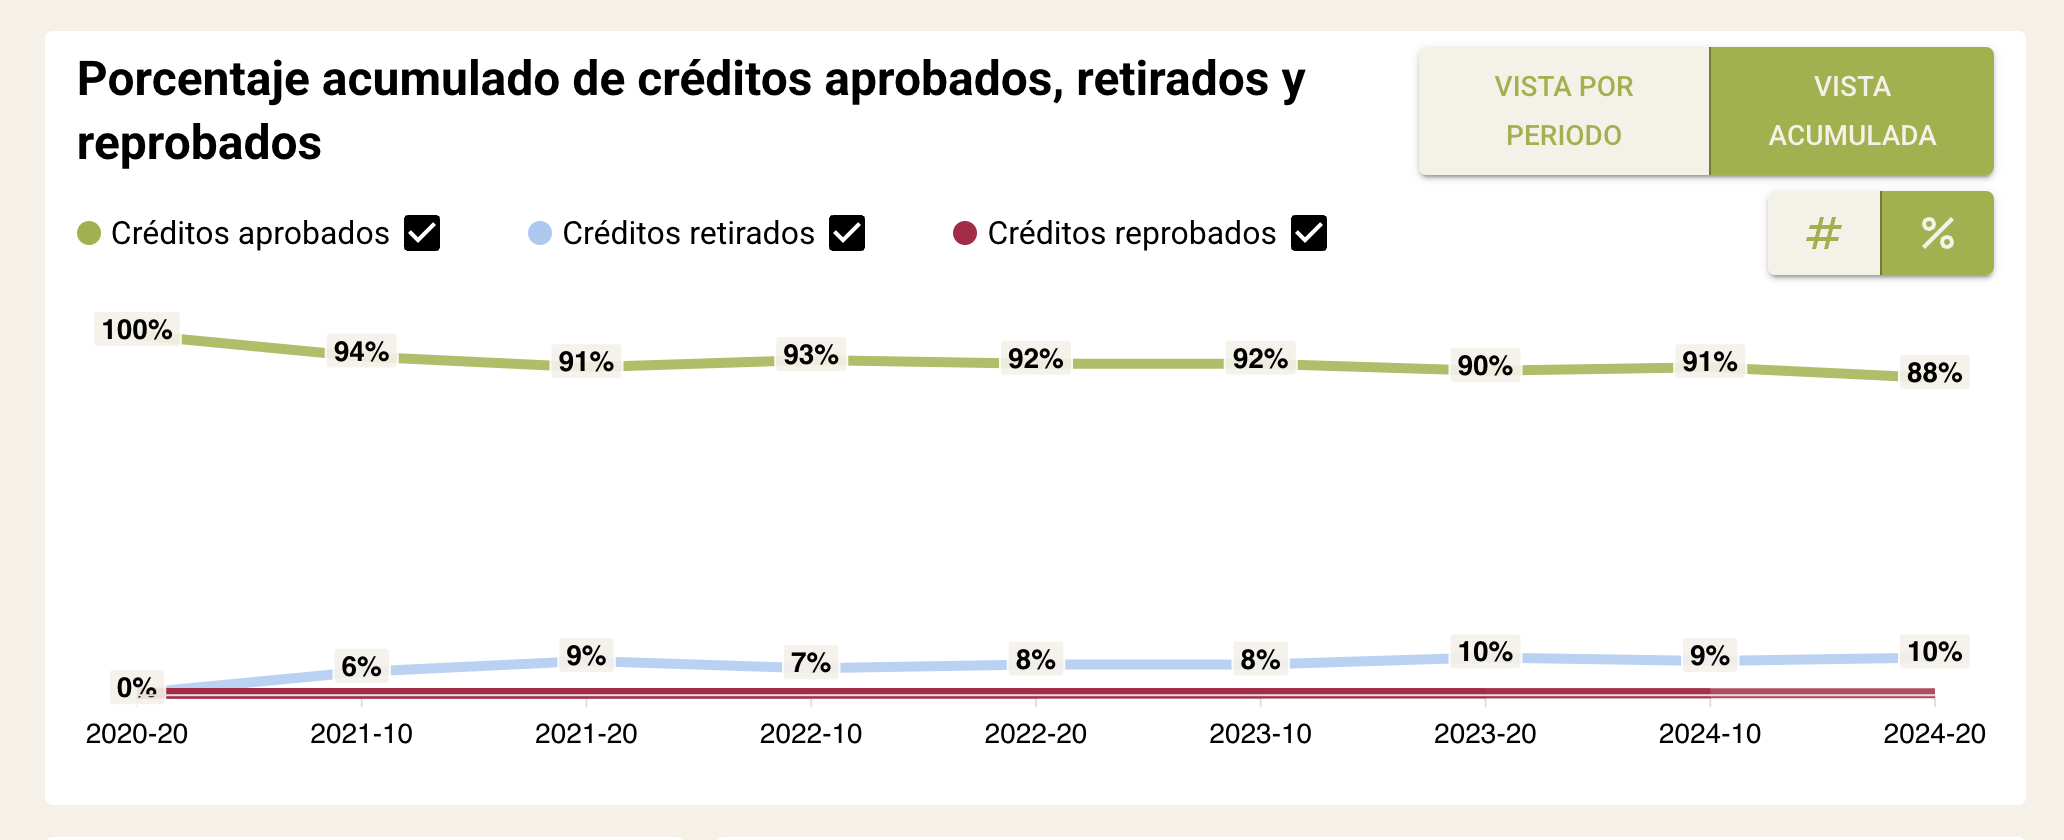
\includegraphics[width=0.8\textwidth]{assets/nes/creditos_acumulados.png}
		      \caption{Gráfica de créditos por periodo en vista acumulada.}
		      \label{fig:creditos_acumulados}
	      \end{figure}

	\item \textbf{Vista porcentual o absoluta.} Al igual que la tabla de créditos inscritos, la gráfica de créditos por periodo permite al usuario alternar entre una vista porcentual y una vista absoluta. La vista porcentual es particularmente útil para comparar el comportamiento de los créditos aprobados, retirados y reprobados en cada periodo académico, independientemente del número total de créditos inscritos. Las figuras \ref{fig:creditos_retirados} y \ref{fig:creditos_acumulados} constituyen ejemplos de la gráfica de créditos por en vista porcentual, mientras que la figura \ref{fig:grafica_creditos} muestra la gráfica en vista absoluta.
\end{itemize}

\paragraph{Condiciones académicas} En la parte inferior izquierda de la pestaña de Desempeño, se presenta la cantidad de suspensiones académicas, pruebas académicas, pruebas de reingreso e incompletos totales que el estudiante ha tenido a lo largo de su carrera. Se muestra en la figura \ref{fig:condiciones_academicas}. Es un componente simple, al que la interactividad no le agregaría valor, pero constituye una pieza de información crucial para el usuario, sobretodo si el conteo de alguno de esos indicadores es mayor a cero.

\begin{figure}[H]
	\centering
	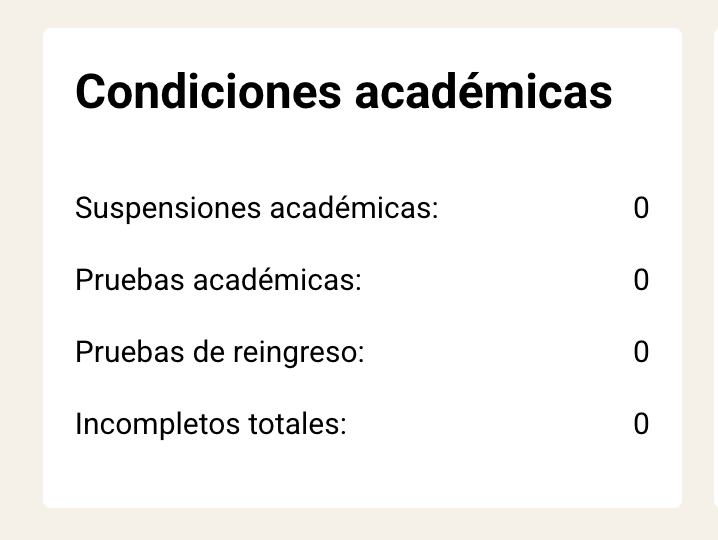
\includegraphics[width=0.4\textwidth]{assets/nes/condiciones_academicas.png}
	\caption{Condiciones académicas.}
	\label{fig:condiciones_academicas}
\end{figure}

\paragraph{Resultados del ICFES} En la parte inferior derecha de la pestaña, se resume el desempeño del estudiante en el examen de estado Saber Pro, como se puede evidenciar en la figura \ref{fig:icfes}. Se presenta el puntaje global del examen, así como los puntajes específicos obtenidos en cada una de las áreas del examen. Se presenta un gráfico de radar que ilustra los puntajes de cada área y permite reconocer las fortalezas y debilidades del alumno un solo vistazo. Este gráfico es interactivo y permite al usuario visualizar los puntajes de cada área al pasar el cursor sobre el gráfico. En esa tarjeta se incluye también el nombre de la institución que otorgó el diploma de bachiller al estudiante en cuestión.

\begin{figure}[H]
	\centering
	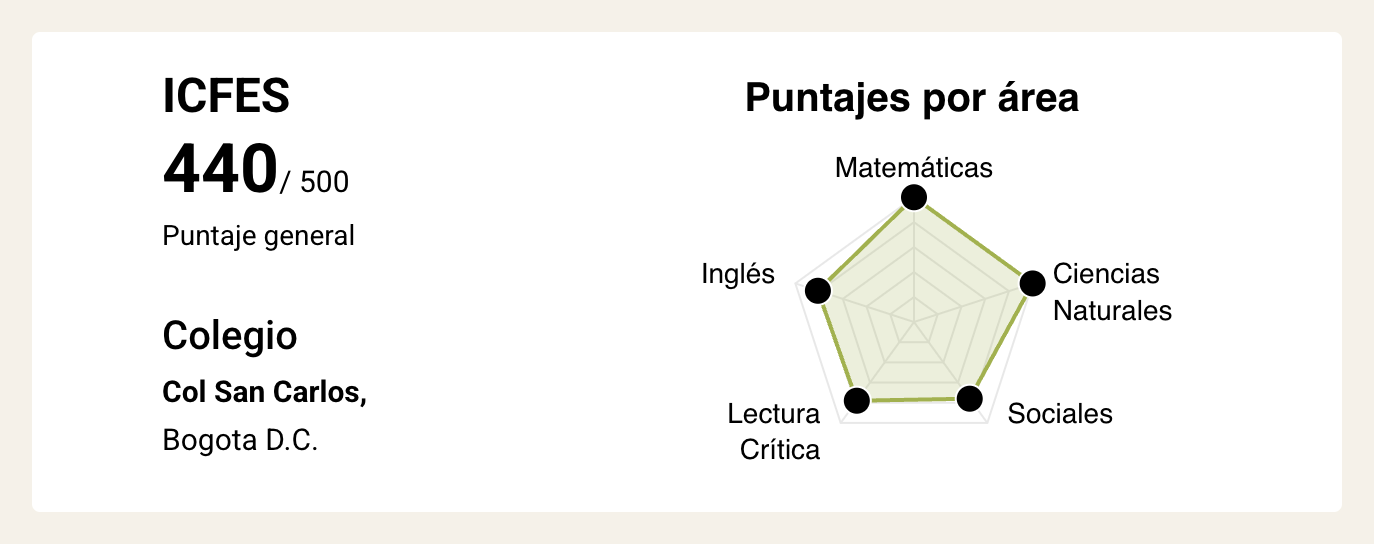
\includegraphics[width=0.8\textwidth]{assets/nes/icfes.png}
	\caption{Resultados del ICFES.}
	\label{fig:icfes}
\end{figure}

\subsubsection{Pestaña de Materias}

La pestaña de Materias presenta un listado de todas las asignaturas que el estudiante ha inscrito a lo largo de su estancia en la Universidad. Consta de dos componentes principales. En la parte superior, mostrada en la figura \ref{fig:filtros_materias}, se encuentra un componente que permite buscar o filtrar materias con facilidad, incluyendo una barra de búsqueda textual y tres filtros: por periodo, por código de área de la materia y por estado de la asignatura (aprobada, retirada, reprobada, pendiente o incompleta). Cada filtro cuenta con un menú desplegable que permite al usuario seleccionar una o varias opciones entre las posibilidades de filtrado. Como ejemplo, la figura \ref{fig:filtro_periodo_materias} muestra el filtro por periodo.

\begin{figure}[H]
	\centering
	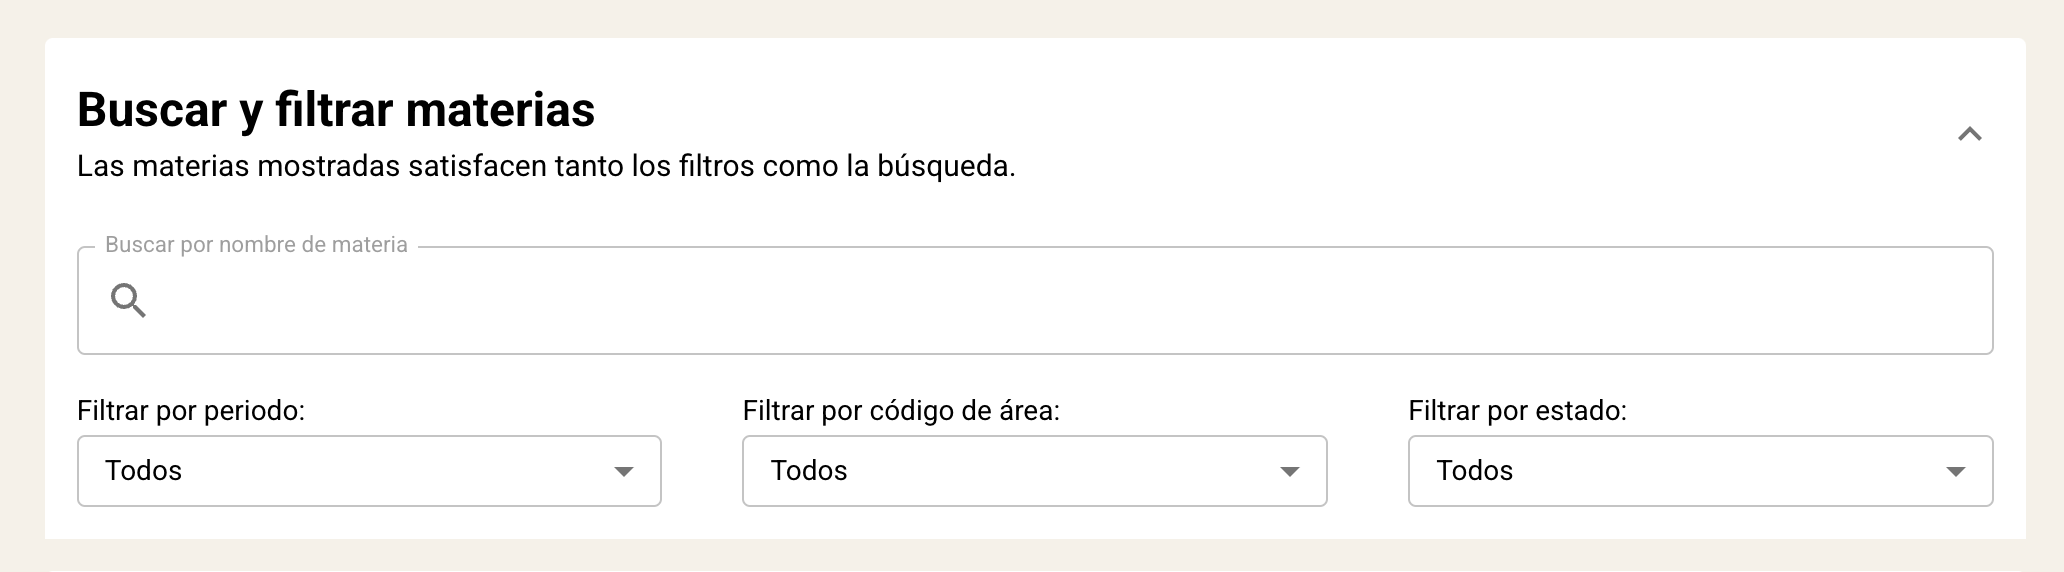
\includegraphics[width=0.8\textwidth]{assets/nes/filtros_materias.png}
	\caption{Componente de búsqueda y filtros de materias.}
	\label{fig:filtros_materias}
\end{figure}

\begin{figure}[H]
	\centering
	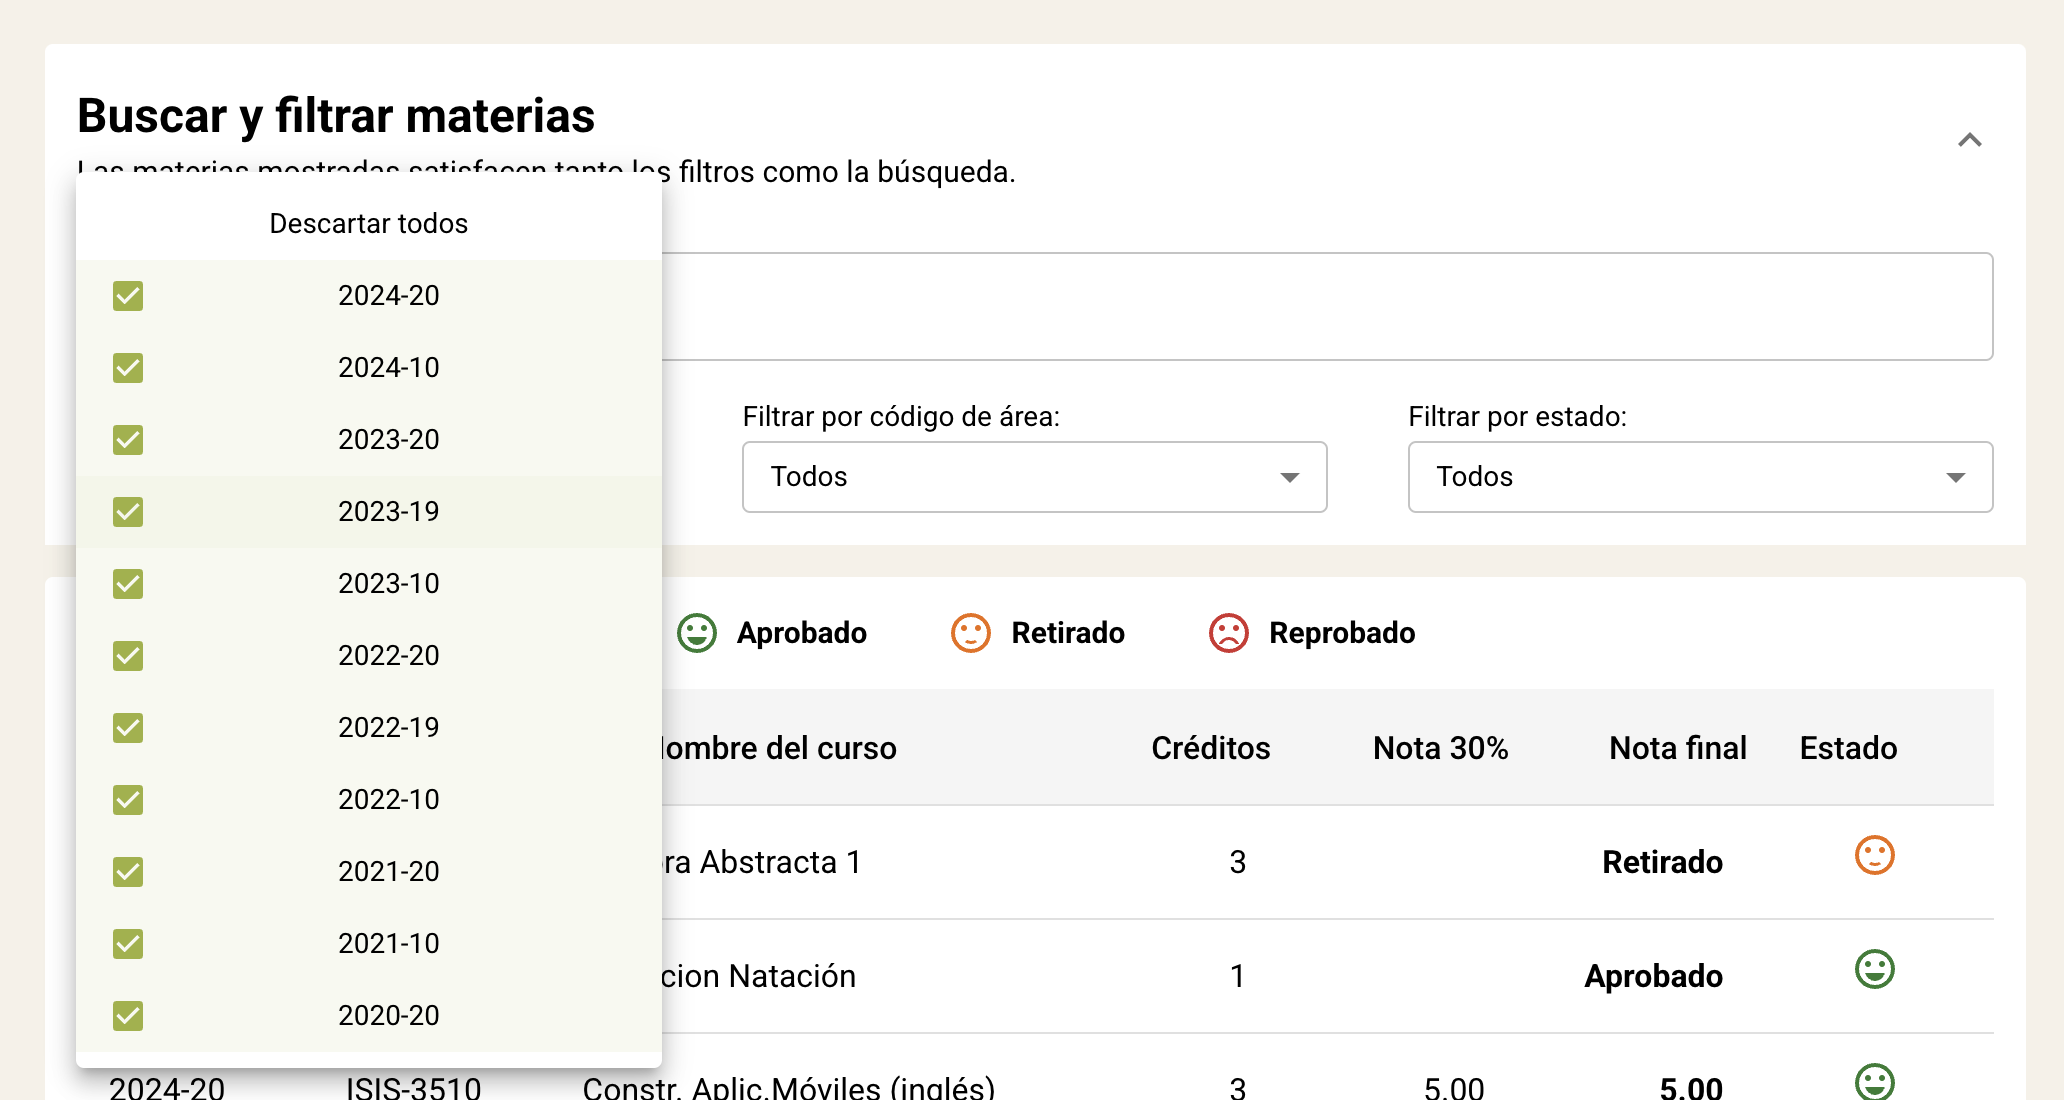
\includegraphics[width=0.8\textwidth]{assets/nes/filtro_periodo_materias.png}
	\caption{Menú desplegable de filtro por periodo en el componente de búsqueda y filtros de materias.}
	\label{fig:filtro_periodo_materias}
\end{figure}

Debajo de ese componente, se encuentra la tabla con el listado de materias, que está en la figura \ref{fig:tabla_materias}. Para cada materia, se muestra el periodo en el que se cursó, el código, el nombre, el número de créditos, la calificación parcial obtenida por el estudiante en el 30\% de la materia, la nota final alcanzada y el estado de la materia. Adicionalmente, las materias que se cursaron de forma virtual están marcadas con un ícono que lo indica. La tabla se puede ordenar por cualquiera de las columnas, permitiendo al usuario visualizar la información de la forma que prefiera, en adición a los filtros y la barra de búsqueda.

\begin{figure}[H]
	\centering
	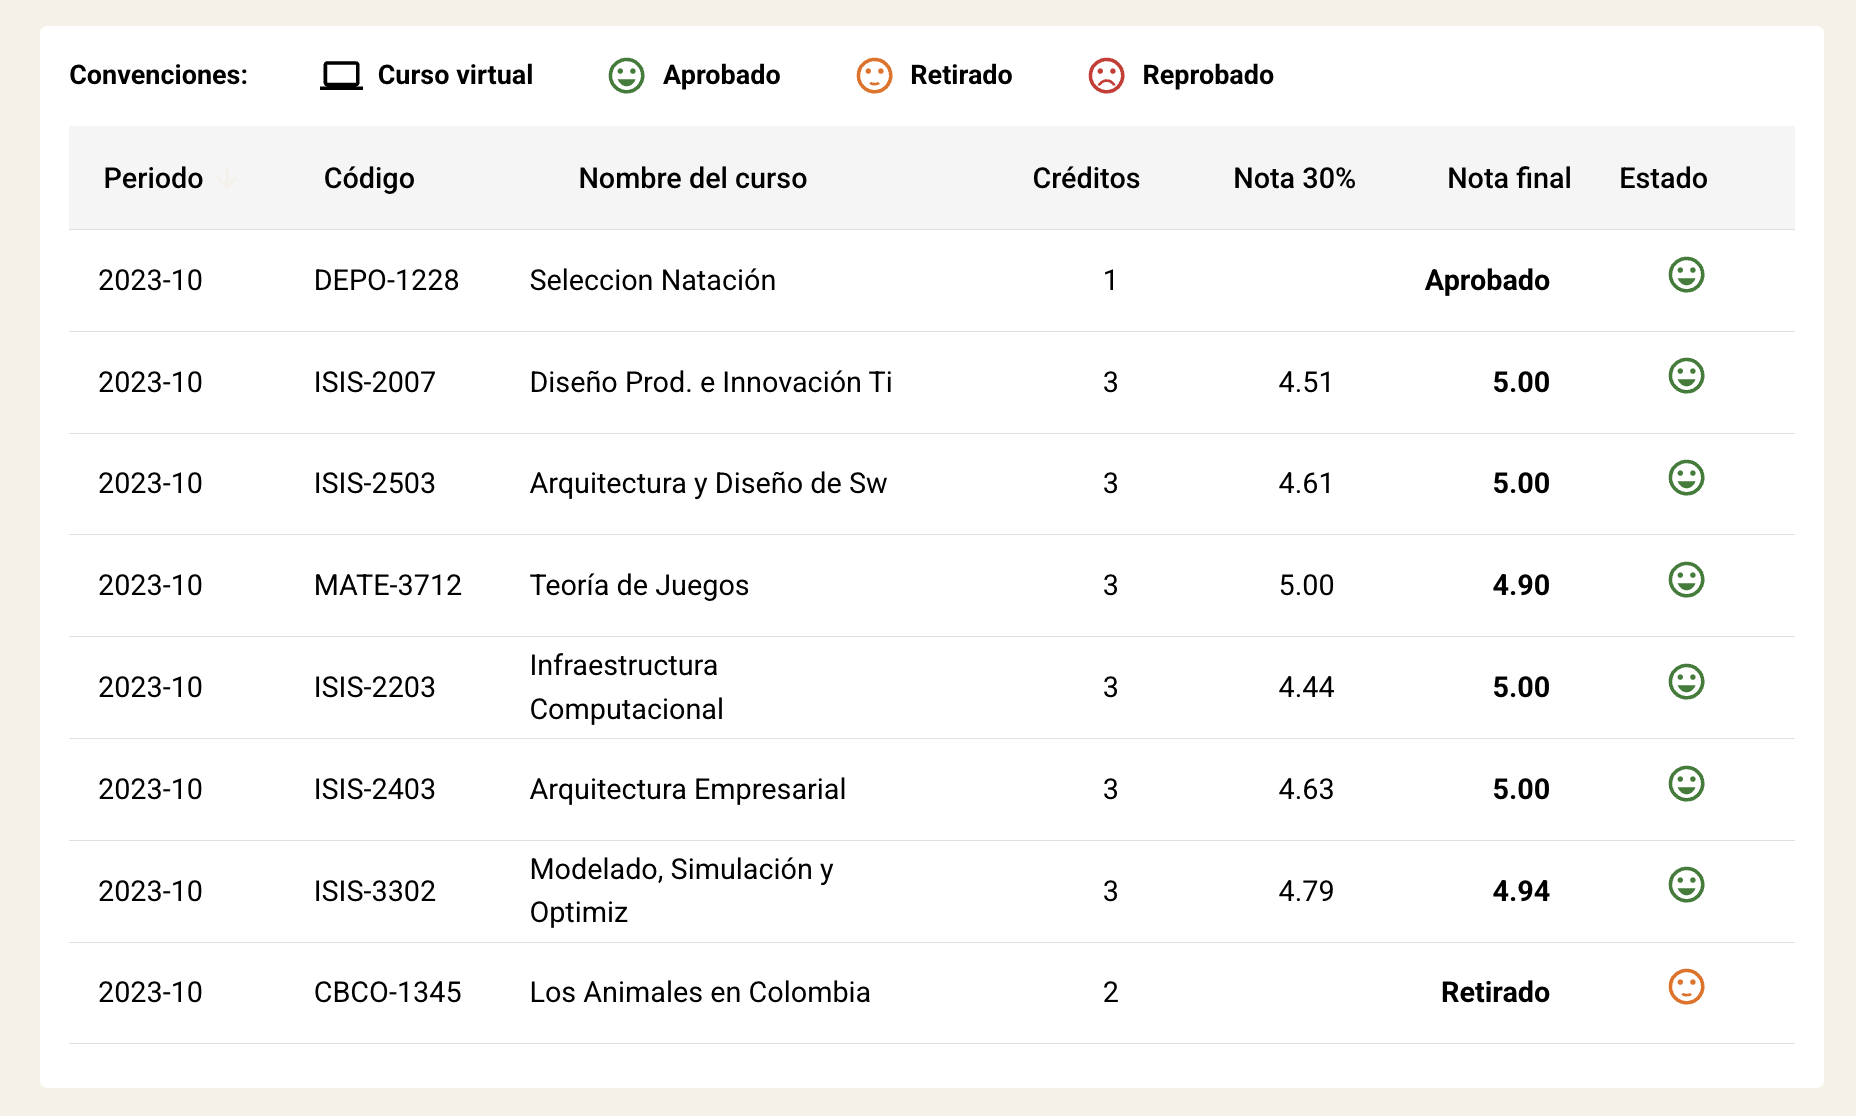
\includegraphics[width=0.8\textwidth]{assets/nes/tabla_materias.png}
	\caption{Tabla de materias inscritas, filtrada para el periodo 2023-10.}
	\label{fig:tabla_materias}
\end{figure}

Esta pestaña permite varios casos de uso distintos sin necesidad de contar con muchos componentes. A continuación, se describen algunos de los más comunes:
\begin{itemize}
	\item Consultar si un estudiante ha cursado o no una materia específica (haciendo uso de la barra de búsqueda) y, en caso de haberla cursado, ver el resultado obtenido.
	\item Visualizar las calificaciones de un estudiante en un área de conocimiento específica, por ejemplo, matemáticas (haciendo uso del filtro por código de área de la materia, en este caso, la opción MATE).
	\item Ver cuántas y cuáles materias han sido reprobadas o retiradas por un estudiante (haciendo uso del filtro por estado de la materia).
	\item Ver las materias que el estudiante cursó en un periodo académico específico y sus resultados, o ver las que se encuentra cursando en el periodo actual (haciendo uso del filtro por periodo).
	\item Consultar todas las materias inscritas por el estudiante en un periodo académico específico.
	\item Conocer las materias en las que el estudiante ha tenido mejor o peor desempeño, ordenando la tabla por la columna de nota final.
\end{itemize}

\subsubsection{Pestaña de Financiación}

La pestaña de Financiación presenta información detallada sobre cómo el estudiante ha financiado sus estudios en la Universidad. Esta pestaña solo es accesible para los directivos de la Universidad, quienes pueden hallarla útil para la toma de decisiones relacionadas con el otorgamiento de apoyos financieros.

La pestaña contiene dos piezas fundamentales de información:
\begin{itemize}
	\item El estrato socioeconómico del estudiante. En Colombia, \say{la estratificación socioeconómica es una clasificación en estratos de los inmuebles residenciales que deben recibir servicios públicos. Se realiza principalmente para cobrar de manera diferencial por estratos los servicios públicos domiciliarios permitiendo asignar subsidios y cobrar contribuciones en esta área.} \cite{estrato}. A causa de eso, es uno de muchos indicadores importantes para determinar la capacidad de pago de un estudiante y, por ende, su necesidad de apoyo financiero.
	\item Un gráfico de barras apiladas con la distribución de la financiación del estudiante en cada periodo académico en el que se ha matriculado. Las barras se dividen en segmentos que representan las distintas fuentes de financiación, como becas, créditos, ahorros, recursos propios, entre otros. Cada segmento se colorea de forma distinta y se etiqueta con el porcentaje de financiación que representa para el periodo en cuestión. La altura de la barra representa el total de la financiación en cada periodo académico, que no necesariamente corresponde al 100\% de la matrícula, pues el estudiante puede haber cursado matrículas parciales.
\end{itemize}
Un ejemplo de la pestaña de Financiación se muestra en la figura \ref{fig:financiacion}.

\begin{figure}[H]
	\centering
	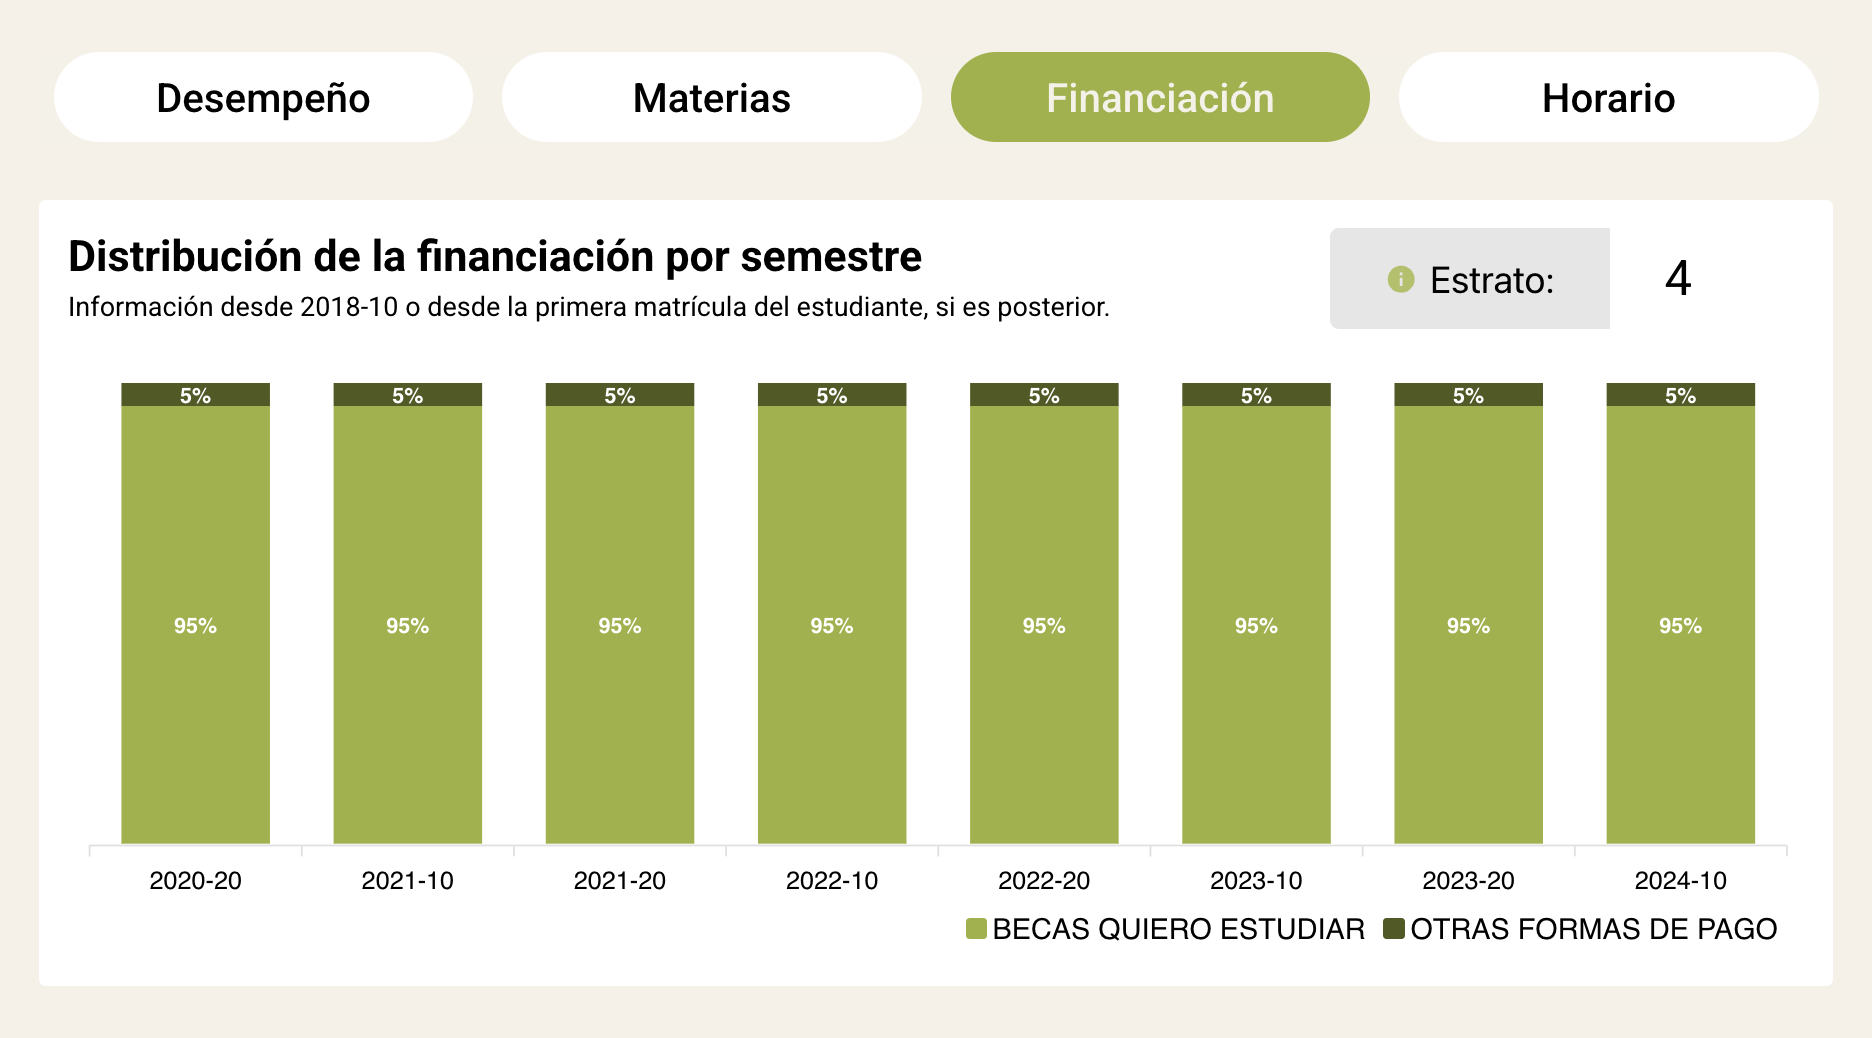
\includegraphics[width=0.8\textwidth]{assets/nes/financiacion.png}
	\caption{Pestaña de Financiación.}
	\label{fig:financiacion}
\end{figure}

\subsubsection{Pestaña de Horario}

La pestaña de Horario presenta el horario de clases del estudiante en el momento de la consulta. El horario se muestra en un formato clásico de horario de clases, como se puede evidenciar en la figura \ref{fig:horario}, donde cada columna representa un día de la semana y cada fila representa una franja de media hora. Cada celda de la tabla contiene la información de la materia que el estudiante tiene programada en ese día y a esa hora.

\begin{figure}[H]
	\centering
	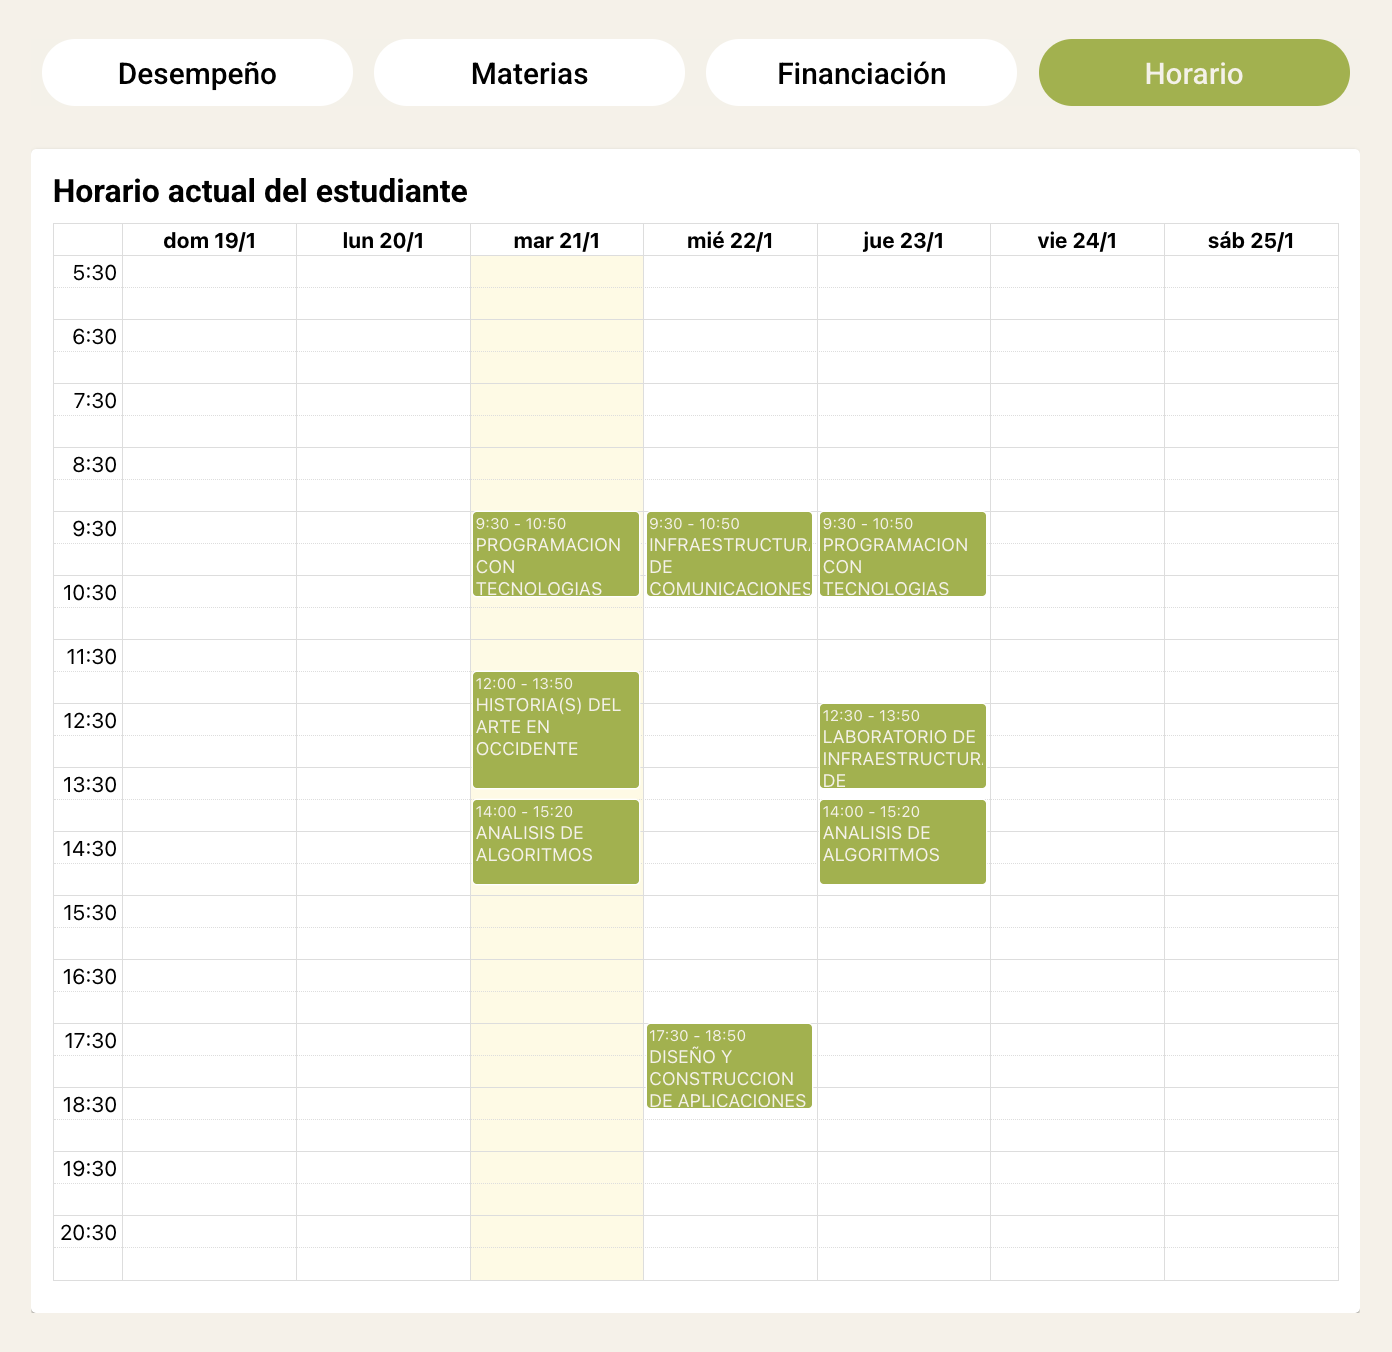
\includegraphics[width=0.8\textwidth]{assets/nes/horario.png}
	\caption{Horario de clases de un estudiante anónimo.}
	\label{fig:horario}
\end{figure}

Al pulsar en una celda de la tabla, se despliega una ventana emergente con información detallada de la materia, incluyendo el código de la materia, el nombre de la materia, el nombre del profesor, el salón de clases y el tipo de clase (magistral, complementaria, laboratorio, taller, entre otros). En caso de que el estudiante tenga una materia virtual programada, aparece un ícono que lo indica. Se muestra la información de una materia en la figura \ref{fig:detalle_horario}.

\begin{figure}[H]
	\centering
	
\includegraphics[width=0.8\textwidth]{assets/nes/detalle_horario.png}
	\caption{Detalle de una materia en el horario de un estudiante anónimo.}
	\label{fig:detalle_horario}
\end{figure}

Esta pestaña es naturalmente útil para los estudiantes, particularmente al inicio de cada semestre, cuando deben organizar su tiempo y coordinar sus actividades. Sumado a eso, la pestaña es de gran utilidad para los profesores, quienes pueden visualizar el horario de sus estudiantes y coordinar reuniones, tutorías y otros eventos con ellos. Para servir a ese fin, el horario cambia dinámicamente cada semana como respuesta a modificaciones en los horarios de clase, por ejemplo, a causa de días festivos o de eventos organizados por la Universidad.

\subsubsection{Información específica para estudiantes en riesgo académico}

En el diseño del Perfil del estudiante, se incorporó una funcionalidad específica para alertar sobre estudiantes que cumplen algún criterio de riesgo académico. Actualmente, se identifican cinco criterios de riesgo académico, que son los siguientes:
\begin{itemize}
	\item El estudiante está en segundo semestre y tiene un PGA entre 3.00 y 3.30.
	\item El estudiante está en tercer semestre o superior y tiene un PGA entre 3.25 y 3.50.
	\item El estudiante pagó matrícula completa, pero tiene inscritos menos de 13 créditos.
	\item El estudiante ha retirado $x$ materias en el semestre actual.
	\item El estudiante va perdiendo $x$ materias al corte del 30\%.
\end{itemize}

En los últimos dos criterios, la $x$ corresponde al número de materias en cuestión, de acuerdo con la realidad del estudiante. Esos dos criterios se muestran únicamente en caso de que la cantidad de materias sea de 3 o más. Ese valor es parametrizable y puede ser ajustado a conveniencia por los directivos de la Universidad.

En caso de que el alumno satisfaga alguno de esos criterios, se presenta un mensaje de alerta en la parte superior de la pestaña de Desempeño, indicando con gran visibilidad el riesgo académico correspondiente. La figura \ref{fig:riesgo_academico} presenta un ejemplo de un estudiante con riesgo académico. Estos riesgos se muestran a cualquier profesor o administrativo que consulte el perfil, así como también al estudiante cuando consulta su propio perfil.

\begin{figure}[H]
	\centering
	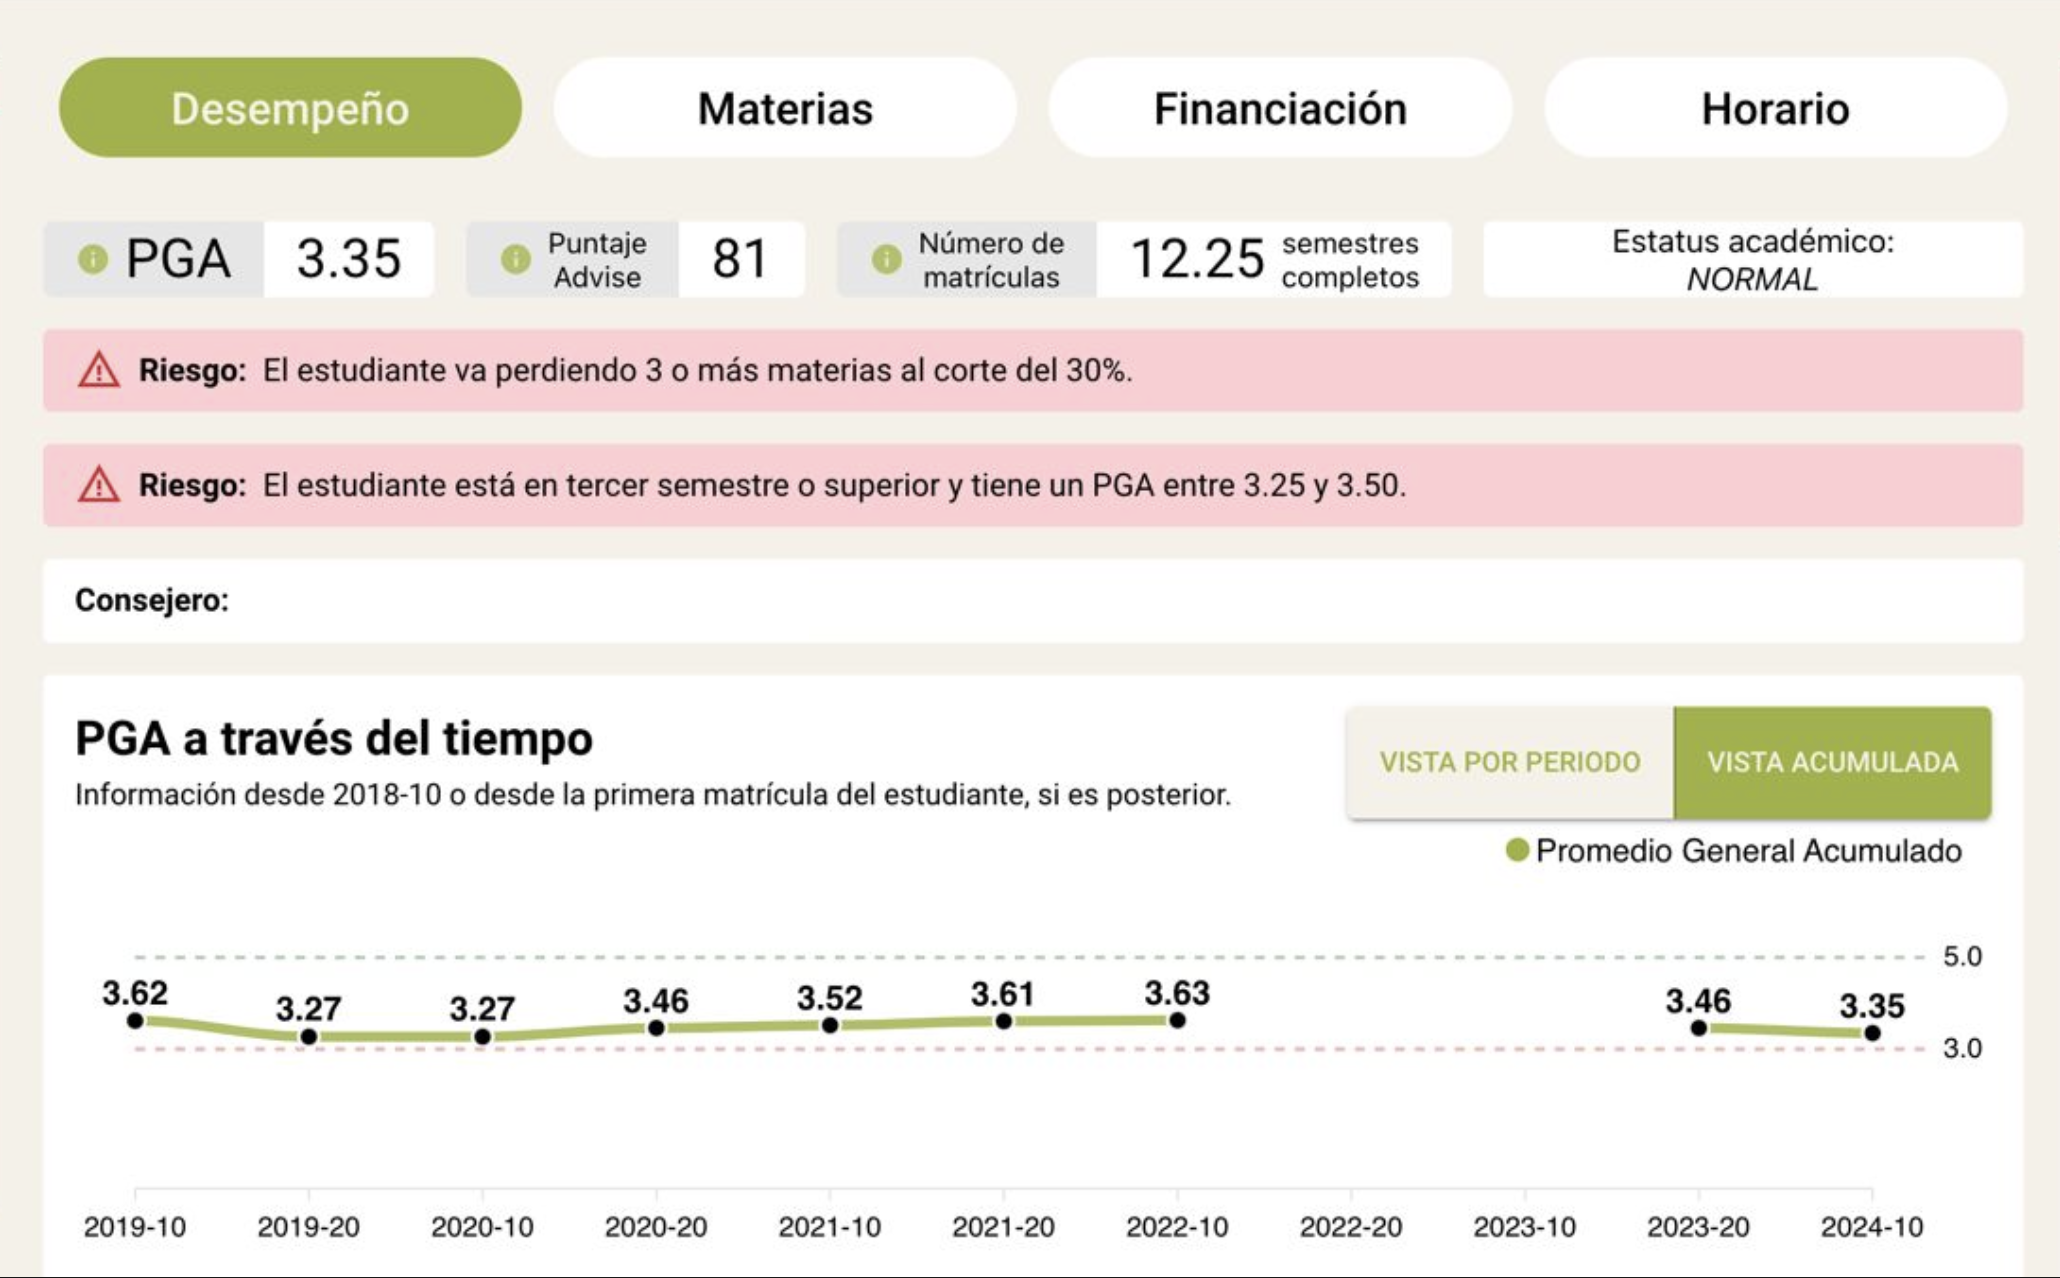
\includegraphics[width=0.8\textwidth]{assets/nes/riesgo_academico.png}
	\caption{Mensaje de alerta de riesgo académico en el perfil de un estudiante anónimo.}
	\label{fig:riesgo_academico}
\end{figure}

\subsubsection{Información específica para estudiantes graduados}

En el Perfil del estudiante se agregó información específica para estudiantes graduados. En la pestaña de Desempeño, se presenta un mensaje que exalta el logro de haberse graduado y exhibe el título obtenido, con el mes y año en el que se obtuvo. En caso de que el alumno haya completado alguna opción académica, se registra la compleción de la opción, como se puede ver en la figura \ref{fig:graduado}.

\begin{figure}[H]
	\centering
	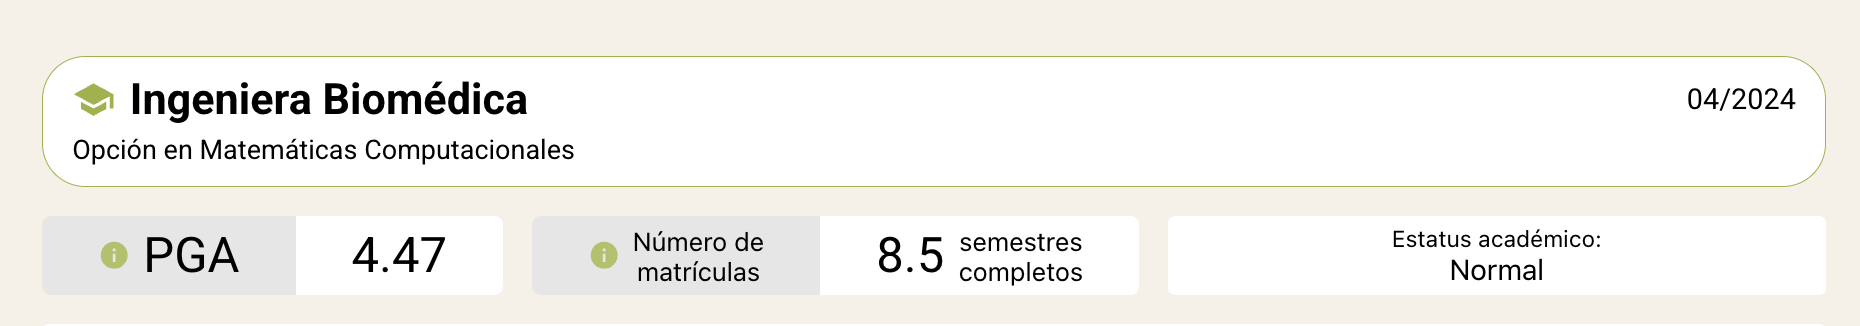
\includegraphics[width=0.8\textwidth]{assets/nes/graduado.png}
	\caption{Mensaje de graduación en el perfil de un estudiante anónimo.}
	\label{fig:graduado}
\end{figure}

Sumado a eso, en caso de que haya sido galardonado durante la carrera o se haya graduado con honores, se resalta ese logro. Un ejemplo de un estudiante graduado con honores está en la figura \ref{fig:graduado_honores}.

\begin{figure}[H]
	\centering
	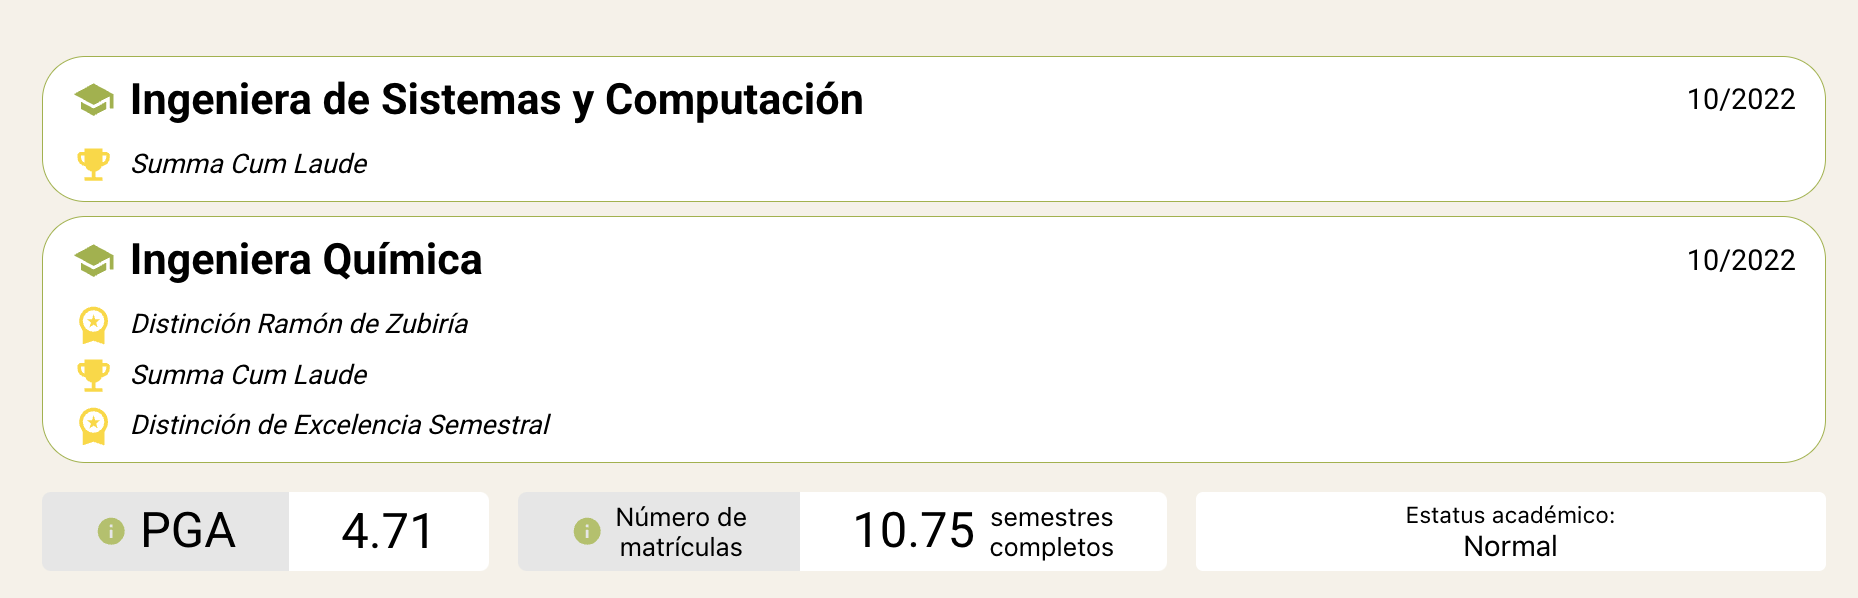
\includegraphics[width=0.8\textwidth]{assets/nes/graduado_honores.png}
	\caption{Mensaje de graduación con honores en el perfil de un estudiante anónimo.}
	\label{fig:graduado_honores}
\end{figure}
